%%%%%%%%%%%%%%%%%%%%%%%%%%%%%%%%%%%%%%%%%%%%%%%%%%%%%%%%%%%%
%%% LIVECOMS ARTICLE TEMPLATE FOR BEST PRACTICES GUIDE
%%% ADAPTED FROM ELIFE ARTICLE TEMPLATE (8/10/2017)
%%%%%%%%%%%%%%%%%%%%%%%%%%%%%%%%%%%%%%%%%%%%%%%%%%%%%%%%%%%%
%%% PREAMBLE
\documentclass[9pt,tutorial,pubversion]{livecoms}
% Use the 'onehalfspacing' option for 1.5 line spacing
% Use the 'doublespacing' option for 2.0 line spacing
% Use the 'lineno' option for adding line numbers.
% The 'bestpractices' option for indicates that this is a best practices guide.
% Omit the bestpractices option to remove the marking as a LiveCoMS paper.
% Please note that these options may affect formatting.

\usepackage{lipsum} % Required to insert dummy text
\usepackage[version=4]{mhchem}
\usepackage{siunitx}
\usepackage{textcomp}
%\usepackage{soul}	%% for markup in revision, to use \hl
\usepackage{listings}
\lstset{
	basicstyle=\ttfamily,
	commentstyle={},
	breakatwhitespace=true,
	breaklines=true,
	language=bash
}
\DeclareSIUnit\Molar{M}
\usepackage[italic]{mathastext}
\graphicspath{{figures/}}
\DeclareGraphicsExtensions{.png,.eps}

%%%%%%%%%%%%%%%%%%%%%%%%%%%%%%%%%%%%%%%%%%%%%%%%%%%%%%%%%%%%
%%% IMPORTANT USER CONFIGURATION
%%%%%%%%%%%%%%%%%%%%%%%%%%%%%%%%%%%%%%%%%%%%%%%%%%%%%%%%%%%%

\newcommand{\versionnumber}{1.0}  % you should update the minor version number in preprints and major version number of submissions.
\newcommand{\githubrepository}{\url{https://github.com/jalemkul/gmx_tutorials_livecoms}}  %this should be the main github repository for this article

\newcommand{\urlstring}{http://www.mdtutorials.com/gmx}
\newcommand{\tutorialhomeurl}{\url{\urlstring}}
\newcommand{\tutoriallyso}{\url{\urlstring/lysozyme}}
\newcommand{\tutorialkalp}{\url{\urlstring/membrane_protein}}
\newcommand{\tutorialpmf}{\url{\urlstring/umbrella}}
\newcommand{\tutorialbiphasic}{\url{\urlstring/biphasic}}
\newcommand{\tutorialcomplex}{\url{\urlstring/complex}}
\newcommand{\tutorialfes}{\url{\urlstring/free_energy}}
\newcommand{\tutorialvsite}{\url{\urlstring/vsites}}

\newcommand{\norm}[1]{\left\lVert#1\right\rVert}

%%%%%%%%%%%%%%%%%%%%%%%%%%%%%%%%%%%%%%%%%%%%%%%%%%%%%%%%%%%%
%%% ARTICLE SETUP
%%%%%%%%%%%%%%%%%%%%%%%%%%%%%%%%%%%%%%%%%%%%%%%%%%%%%%%%%%%%
\title{From Proteins to Perturbed Hamiltonians: A Suite of Tutorials for the GROMACS-2018 Molecular Simulation Package [Article v\versionnumber]}

\author[1*]{Justin A. Lemkul}
% \author[1,2\authfn{1}\authfn{3}]{Firstname Middlename Familyname}
% \author[2\authfn{1}\authfn{4}]{Firstname Initials Surname}
% \author[2*]{Firstname Surname}
\affil[1]{Department of Biochemistry, Virginia Tech, Blacksburg, VA, United States of America}
% \affil[2]{Institution 2}

% Correspondence emails.  FMS and FS are the appropriate authors initials.
\corr{jalemkul@vt.edu}{JAL}
% \corr{email2@example.com}{FS}

% \contrib[\authfn{1}]{These authors contributed equally to this work}
% \contrib[\authfn{2}]{These authors also contributed equally to this work}

% \presentadd[\authfn{3}]{Department, Institute, Country}
% \presentadd[\authfn{4}]{Department, Institute, Country}

\blurb{This LiveCoMS document is maintained online on GitHub at \githubrepository; to provide feedback, suggestions, or help improve it, please visit the GitHub repository and participate via the issue tracker.}

%%%%%%%%%%%%%%%%%%%%%%%%%%%%%%%%%%%%%%%%%%%%%%%%%%%%%%%%%%%%
%%% PUBLICATION INFORMATION
%%% Fill out these parameters when available
%%% These are used when the "pubversion" option is invoked
%%%%%%%%%%%%%%%%%%%%%%%%%%%%%%%%%%%%%%%%%%%%%%%%%%%%%%%%%%%%
\pubDOI{10.XXXX/YYYYYYY}
\pubvolume{<volume>}
\pubyear{<year>}
\articlenum{<number>}
\datereceived{Month, Day, Year}
\dateaccepted{Month, Day, Year}

%%%%%%%%%%%%%%%%%%%%%%%%%%%%%%%%%%%%%%%%%%%%%%%%%%%%%%%%%%%%
%%% ARTICLE START
%%%%%%%%%%%%%%%%%%%%%%%%%%%%%%%%%%%%%%%%%%%%%%%%%%%%%%%%%%%%

\begin{document}

\begin{frontmatter}
\maketitle

\begin{abstract}
% In your work, in this particular slot, please provide an abstract of no more than 250 words.
% Your abstract should explain the main contributions of your article, and should not contain any material that is not included in the main text.
% Please note that your abstract, plus the authorship material following it, must not extend beyond the title page or modifications to the LaTeX class will likely be needed.

Molecular dynamics (MD) simulations are a popular technique for studying the atomistic behavior of any molecular system. Performing MD simulations requires a user to become familiar with the commands, options, and file formats of the chosen simulation software, none of which are consistent across different programs. Beyond these requirements, users are expected to be familiar with various aspects of physics, mathematics, computer programming, and interaction with a command-line environment, presenting critical barriers to entry in the MD simulation field. This article presents seven tutorials for instructing users in the proper methods for preparing and carrying out different types of MD simulations in the popular GROMACS simulation package. GROMACS is an open-source, free, and flexible MD package that is consistently among the fastest in the world. The tutorials presented here range from a "simple" system of a protein in aqueous solution to more advanced concepts such as force field organization and modification for a membrane-protein system, two methods of calculating free energy differences (umbrella sampling and "alchemical" methods), biphasic systems, protein-ligand complexes, and the use of virtual sites in MD simulations. In this article, users are provided the rationale and a theoretical explanation for the command-line syntax in each step in the online tutorials (available at \tutorialhomeurl) and the underlying settings and algorithms necessary to perform robust MD simulations in each scenario.

\end{abstract}

\end{frontmatter}


\section{Introduction}

% Here you would explain what problem you are tackling and briefly motivate your work.

% In this particular template, we have removed most of the usage examples which occur in \texttt{sample-document.tex} to provide a minimal template you can modify; however, we retain a couple of examples illustrating more unusual features of our templates/article class, such as the checklists, and information on algorithms and pseudocode.

Molecular dynamics (MD) simulations are widely applied to studies of structure-function relationships, disease pathways, and drug design. MD simulations rely on the relationship between a given configuration of atoms and its energy to propagate dynamics. This process is driven by empirical force fields, energy functions and associated parameter sets that are used to compute energies and forces acting in a given configuration. After calculating the forces, the configuration is updated by applying those forces over a discrete time step, $\delta$t. An assembly of many configurations, linked through time, establishes a trajectory for subsequent visualization and analysis.

Performing an MD simulation requires that many choices be made, including the starting structure of the molecule(s) of interest, the force field model to be applied, concentration and nature of salt in solution, the integration method, algorithms for temperature and/or pressure regulation, and length of the simulation itself. This complex series of decisions will dictate the quality, reliability, and reproducibility of the simulation, and consequently should be undertaken only after careful consideration. Beyond the conceptual issues lies the interface with the MD simulation package itself. The user must translate the knowledge of the experimental setup to actual practice by implementing these details in the framework of a complex software suite. The combination of these factors can be burdensome for new users, who may be prone to making errors or failing to consider best practices and subtle nuances of a large body of literature.

The GROMACS simulation package~\cite{Hess2008,Abraham2015} is an open-source software suite that is free for all users and available worldwide. GROMACS has for many years been among the fastest MD codes available~\cite{Hess2008}, making it a popular choice for carrying out MD simulations as hardware and algorithmic development allow for ever-increasing trajectory lengths.

\subsection{Scope}

% Tutorials should endeavor to cover the specific task at hand, and also highlight how the steps might need to be modified (or additional care might need to be taken at particular points) to handle more general cases.

% The scope of the tutorial, as well as the expected proficiencies / outcomes for researchers who complete the tutorial, should be clearly defined.
% This will often happen in a specific section or subsection in the article itself.

% Define objectives for each tutorial, refer back in each section
The seven tutorials presented here range in difficulty from basic to advanced, roughly in the order of presentation. Each of the tutorials comes with its own learning objectives and expected outcomes.

After completing Tutorial 1, "Lysozyme in Water," the user should be able to build a solvated protein system and carry out a short MD simulation. Specific learning objectives include:
\begin{enumerate}
	\item Understand the content of a GROMACS system topology
	\item Carry out basic steps of setting up a periodic system, including solvation and adding ions
	\item Identify keywords and typical settings in \texttt{.mdp} input files
	\item Control position restraints and topology directives via \texttt{.mdp} settings
	\item Determine the appropriate algorithms for energy-minimizing and equilibrating a biomolecular system and performing a production MD simulation
\end{enumerate}

After completing Tutorial 2, "KALP\textsubscript{15} in DPPC," the user should be able to build a simple membrane-protein system containing one lipid type. Specific learning objectives include:
\begin{enumerate}
	\item Understand the organization and contents of GROMACS force field files and how parameters from different, but compatible, sources can be added to them
	\item Apply an iterative packing routine to place phospholipids around a transmembrane protein
	\item Perform lipid-specific analysis using custom index groups
\end{enumerate}

After completing Tutorial 3, "Umbrella Sampling," the user should be able to perform simulations under the influence of a biasing potential. Specific learning objectives include:
\begin{enumerate}
	\item Apply \texttt{.mdp} keywords that invoke the pull code to add a simple, one-dimensional biasing potential to selected atoms in a system
	\item Define what is meant by a "reaction coordinate" and how to construct a suitable one
	\item Perform restrained simulations in multiple sampling windows along a reaction coordinate
	\item Compute a potential of mean force profile
\end{enumerate}

After completing Tutorial 4, "Biphasic Systems," the user should be able to construct heterogeneous systems of two different liquids. Specific learning objectives include:
\begin{enumerate}
	\item Build a simulation system containing a liquid that is not water
	\item Manipulate the relative positioning of a box within a larger volume
\end{enumerate}

After completing Tutorial 5, "Protein-Ligand Complex," the user should be able to construct a solvated protein system including a ligand that needs to be parametrized. Specific learning objectives include:
\begin{enumerate}
	\item Produce a ligand topology outside of GROMACS and incorporate it into a system topology
	\item Determine how to verify if a ligand topology is suitable for further simulation
	\item Perform analysis of interactions between a protein and a ligand
\end{enumerate}

After completing Tutorial 6, "Free Energy of Solvation," the user should be able to carry out a series of simulations for the alchemical transformation of a small molecule in water. Specific learning objectives include:
\begin{enumerate}
	\item Understand the purpose of \texttt{.mdp} keywords related to free energy calculations
	\item Use the Bennett Acceptance Ratio method to compute the free energy difference of the transformation of van der Waals terms
\end{enumerate}

After completing Tutorial 7, "Virtual Sites," the user should be able to understand what virtual sites are and how they are used in specific cases. Specific learning objectives include:
\begin{enumerate}
	\item Define a virtual site and its position relative to other atoms
	\item Construct a system of a linear molecule with virtual sites
\end{enumerate}

\section{Prerequisites}

% Here you would identify prerequisites/background knowledge that are assumed by your work, as well as any software/license requirements.

The tutorials described in this article assume the user has installed GROMACS, version 2018 or any minor or patch release in the 2018.x series. Instructions for how to install GROMACS can be found in the online manual at \url{http://manual.gromacs.org/documentation/2018-current/index.html}. This tutorial article will not describe how to install GROMACS, as details vary depending on the available hardware, compilers, etc.

\subsection{Background knowledge}
% Tutorials should clearly define what concepts or abilities researchers will need to complete the tutorial (e.g., some proficiency in Python; experience with Jupyter notebooks; knowledge of classical MD; etc).
These tutorials assume the user is familiar with basic Linux or Unix command-line interaction and navigation as well as the use of a plain-text editor such as VIM or Emacs. Background knowledge in MD simulations would be beneficial, though this article seeks to introduce new users to the fundamental concepts that are required to properly execute a simulation. These tutorials cannot be comprehensive in explaining all elements and algorithms in MD simulations, and as such, users are expected to seek outside resources ({\em e.g.}~\cite{Frenkel2001,Leach2001,Kukol2008,Braun2018}) to assist in their understanding. Tutorial 1 (see Section~\ref{lyso}) assumes the user has no experience with GROMACS, and therefore contains the most detail about how to carry out various tasks. In the subsequent six tutorials, it will be assumed that the user is familiar with basic operations and not all steps will be described in depth, except for instances of new or different usage.

Throughout this article, commands that are to be issued by the user are written in \texttt{monospace font} and the command prompt is indicated with \texttt{\$}, which itself is not part of the command the user should enter. Some commands are long and span multiple lines; in these cases the commands should not be entered on separate lines in the terminal, rather as one continuous command. Program and file names are similarly written in \texttt{monospace font} in the text to distinguish them from the narrative.

\subsection{Software/system requirements}
% Tutorials should clearly define what system and/or software requirements the researcher will need to complete the tutorial (e.g., VMD version 1.9 or newer, AMBER, etc.). Tutorials requiring specific software packages must provide instructions and files for the referenced version of the software.
These tutorials assume the user is working with a GROMACS version in the 2018.x series. Other versions have different command-line syntax and input file keywords and attempting to use them will result in problems.

The output of GROMACS analysis programs is, by default, written in a format compatible with XmGrace (\url{http://plasma-gate.weizmann.ac.il/Grace/}). As such, the user should be familiar with plotting data using this program.

For visualization of coordinate files and trajectories, many options are available, including Visual Molecular Dynamics (VMD, \url{http://www.ks.uiuc.edu/Research/vmd/})~\cite{Humphrey1996}, Chimera (\url{https://www.cgl.ucsf.edu/chimera/})~\cite{Petersen2004}, and PyMOL (\url{https://pymol.org/2/}), among others. Users should be familiar with at least one of these programs for visualizing the system. The latest version of each of these programs (VMD 1.9.3, Chimera 1.12, and PyMOL 2.0 at the time this article was written) is preferred for maximum compatibility with different file formats and features.

The protein-ligand complex tutorial will make use of the Avogadro molecular editor (\url{https://avogadro.cc/})~\cite{Hanwell2012} and a Python script that requires a Python 2.7.x version, the NetworkX package in the 1.11.x version series, and any compatible NumPy version. The topology conversion script is not compatible with NetworkX versions in the 2.x series.

\section{Content and Links}

% A tutorial will normally draw on additional files and materials; clearly indicate where and how these are available, with links, and how they are being archived for the long-term and maintained so they stay current.
% You will likely want to reference your GitHub repository as a central point to access all of this information, and then the GitHub repository may link out to other content as needed.

The tutorials described in this article can be accessed at \tutorialhomeurl. All necessary files for completing each tutorial are provided at that location.

\subsection{Overview}

GROMACS comprises a set of programs for preparing, running, and analyzing MD simulations. Each program is called from within a single binary, called \texttt{gmx}, and command-line syntax is similar among all the programs. All options are preceded by a hyphen (-) and the subsequent keyword or filename must be the next argument on the command line. For instance, if a coordinate file is specified as an input file for a given command, \texttt{-f my\_file.pdb} is correct syntax, but separating \texttt{-f} from \texttt{my\_file.pdb} in any way with intervening text or other arguments will cause an error. Some arguments are boolean, meaning that they indicate binary, yes/no choices. For instance, the option \texttt{-princ} (from the \texttt{editconf} command, discussed below), indicates that the user wants the solute molecule to be aligned with its principal axis along the Cartesian {\em x}-axis. The opposite, to not require alignment, would be \texttt{-noprinc}. This syntax is the same for any GROMACS boolean argument.

At any time, the user can refer to help information for a given program by invoking \texttt{gmx help} and the name of the program or use the \texttt{-h} flag. For instance, to read the help information for the \texttt{pdb2gmx} program, the user would type \texttt{gmx help pdb2gmx} or equivalently, \texttt{gmx pdb2gmx -h}.

Every GROMACS program has a set of default options and file names that it assumes it can use if the user does not otherwise specify. That is, if any argument requires a file name (typically input and output files) and one is not provided by the user, the program will look in the working directory for a file with the default name. If that file is not found, then an error is returned. This outcome is often a point of confusion for new users. Refer to the help information for a given program to see what its default file names are, so in the event of an error, it is clear which file is missing. It is generally inadvisable to rely on GROMACS default file names, as they are very generic. The tutorials below all use descriptive file names to encourage best practices in organization and naming conventions.

Each tutorial is available at \tutorialhomeurl, and the link to each specific tutorial is given within each of the following sections. Command-line syntax and input files are available at each tutorial's URL. This article will describe the practical considerations and theoretical basis for the approaches taken here.

%%%%%%%%% TUTORIAL 1 %%%%%%%%%
\subsection{Tutorial 1: Lysozyme in Water} \label{lyso}

\begin{figure}[H]
\centering
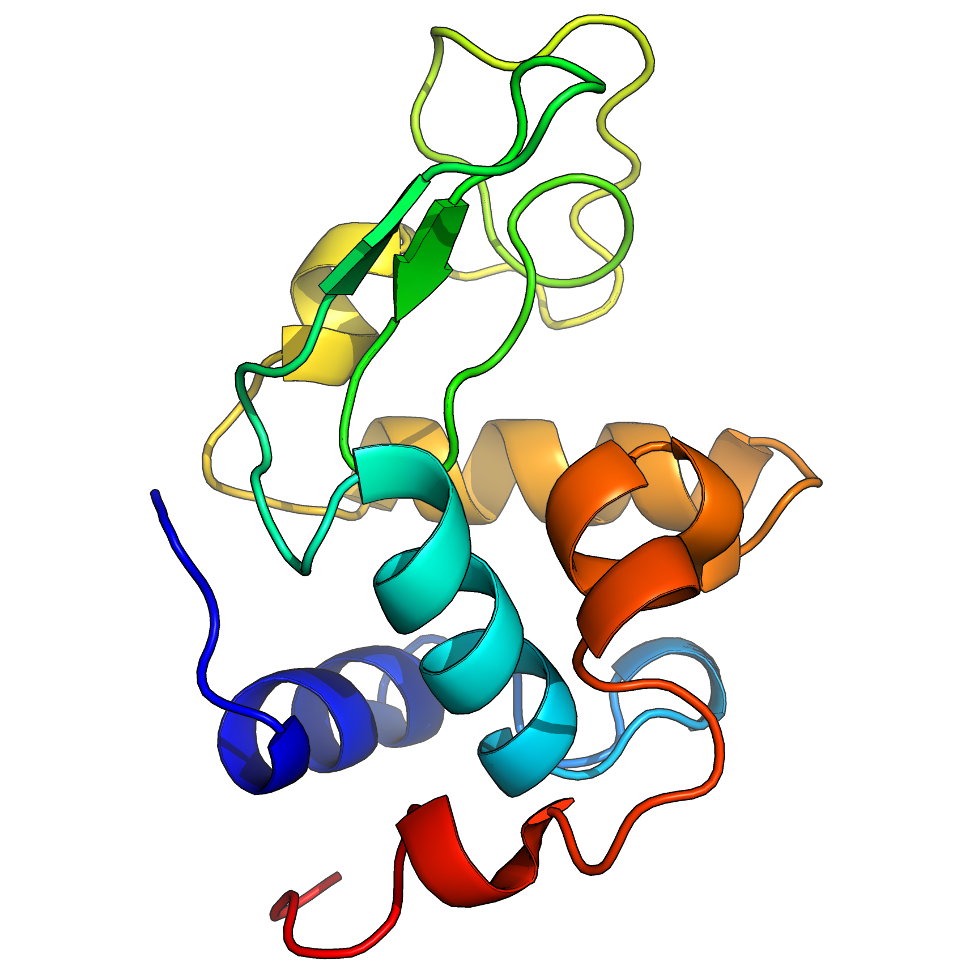
\includegraphics{lysozyme_1aki}
\caption{Crystal structure of hen egg-white lysozyme, taken from PDB 1AKI~\cite{Artymiuk1982}.}
\label{lyso_xtal_fig}
\end{figure}

Many biomolecular simulations involve a solute that is solvated in an aqueous medium or saline solution. Thus, this tutorial guides the user through preparing a system of a protein in water, with counterions. The full tutorial is available at \tutoriallyso. The general protocol for any simulation is to build the coordinates and topology (a description of the properties and connectivity of all atoms in the system), perform energy minimization to relax the coordinates to a low-energy state, equilibrate, and perform a production MD simulation, during which data are collected for subsequent analysis. In this tutorial, the coordinates for the system of interest are for hen egg-white lysozyme (Figure~\ref{lyso_xtal_fig}), which can be downloaded from the Protein Databank, accession code 1AKI~\cite{Artymiuk1982}. For simplicity, the user is instructed to remove crystal waters from the input PDB file:

\begin{lstlisting}
$ grep -v HOH 1aki.pdb > 1AKI_clean.pdb
\end{lstlisting}

Removal of water here is to make the resulting topology less complex. Multiple blocks of water in the topology require manual correction, a task that is not well-suited to new users of the software who are likely unfamiliar with the contents and format of various files. It should be noted, however, that ad hoc removal of crystal waters is not generally a good practice, particularly in instances where a tightly bound water may have some functional significance (structural or catalytic) and must be modeled appropriately.

\subsubsection{Topology Preparation} \label{lyso_top}
The typical approach that GROMACS takes for constructing the topology of a molecular system is to begin with generating a topology for the solute of interest, which is then amended or updated to include other components that are added to the system (water, ions, ligands, etc.). GROMACS uses two types of topology files, one with a \texttt{.top} extension and the other with an \texttt{.itp} extension. There is only ever one \texttt{.top} file for a system, hence it is called the "system topology." A topology with an \texttt{.itp} extension is called an "included topology," indicating that it can be embedded (included) within a system topology to provide the source of other parameters or other molecule definitions.

The GROMACS program most frequently used to write topologies is called \texttt{pdb2gmx}, which reads a coordinate file, determines its contents, and writes a topology for the supplied molecule(s). The name of this program is somewhat misleading, as there is no strict requirement to provide coordinates in PDB format. Refer to the help information for \texttt{pdb2gmx} for allowed formats.

The \texttt{pdb2gmx} program is best suited to linear biopolymers, with limited exceptions for branched (non-linear) bonds. Thus, it is very easy to use \texttt{pdb2gmx} for proteins and nucleic acids, but it is somewhat ill-suited for materials, branched polymers, or complex carbohydrates. However, \texttt{pdb2gmx} can handle common cases such as disulfides and heme linkages. An important point about \texttt{pdb2gmx} is that it can only process species for which parameters have been provided; it does not perform automated parametrization. Therefore, a user must carefully consider what is provided to \texttt{pdb2gmx} before attempting to process a coordinate file. Each force field provided with GROMACS has one or more \texttt{.rtp} (residue topology) files, which contain the parameters and bonded structure for each species supported by the force field. If a given species is not found in a force field \texttt{.rtp} file, \texttt{pdb2gmx} will return a fatal error. Therefore, users must always check the availability of non-standard residues in a given force field to determine its suitability for use.

Many force fields are included in GROMACS, including several variants of the AMBER force field~\cite{Cornell1994,Kollman1996,Wang2000,Garcia2002,Duan2003,Hornak2006,LindorffLarsen2010}, CHARMM22/CMAP for proteins~\cite{MacKerell1998,MacKerell2004} and CHARMM27 for nucleic acids~\cite{Foloppe2000,MacKerell2000}, several GROMOS96 parameter sets~\cite{Daura1998,Schuler2001,Oostenbrink2004,Schmid2011}, and OPLS-AA~\cite{Kaminski2001}. Also note that the CHARMM36 force field~\cite{Best2012,Hart2012,Denning2011,Klauda2010,Huang2016} is available in GROMACS format from \url{http://mackerell.umaryland.edu/charmm_ff.shtml#gromacs}.

Beyond the consideration of whether or not a force field has parameters for a given chemical species, it is important to realize that the choice of force field is perhaps the single most critical aspect to beginning a new simulation project. No existing force field perfectly treats all species, and each available force field has pros and cons for different species. It is incumbent upon the user to make an informed, justifiable choice based on literature reading and evaluation of the force field parametrization protocol to understand to which purposes a given force field is best suited. There is no catch-all answer or universally "best" force field.

Once a starting structure has been chosen and the choice of force field decided upon, run \texttt{pdb2gmx} to create the topology:

\begin{lstlisting}
$ gmx pdb2gmx -f 1AKI_clean.pdb -o 1AKI_processed.gro -water spce
\end{lstlisting}

The first prompt is for the user to select the force field that will be applied to the system. For this tutorial, choose option 15 for OPLS-AA, a widely used all-atom force field. An all-atom force field is used here for simplicity rather than introducing concepts of implicit hydrogen atoms as in united-atom force fields or coarse-grain representations. In principle, many of the force fields provided with GROMACS would be adequate for the purposes of this tutorial. The next choice the user must make is the water model that is to be used. In the tutorial, the \texttt{-water} argument is invoked from \texttt{pdb2gmx} to select the SPC/E water mode~\cite{Berendsen1987}; if this option is not given on the command line, the user is prompted for an interactive choice. The water model is another important consideration, though one over which the user has less freedom. Each force field was parametrized for use with a specific water model. Therefore, the user is not entirely free to choose whichever model happens to be available without due consideration. GROMACS provides a suggested water model for each force field; unless there is good evidence to choose another model, the user should follow this recommendation for greatest accuracy. However, some studies have shown that different biomolecular force fields may be accurately combined with other water models, as is the case in this tutorial. The OPLS-AA force field was originally parametrized for use with the TIP3P water model~\cite{Jorgensen1983}, but it was subsequently shown that the combination of OPLS-AA with SPC/E yielded more accurate hydration free energies for protein side chains~\cite{Hess2006}, suggesting this combination is a sufficiently accurate and self-consistent model for simulating proteins. In the absence of any sufficiently strong justification or precedent, the user should always choose the recommended water model listed by \texttt{pdb2gmx}.

Often, new users are confused at having to choose a water model at this stage, particularly in the case that their provided coordinate file only contains a biomolecule such as a protein. The water model selection is planning for the subsequent steps, in which this solute is hydrated and a force field choice should be made ahead of time. By selecting the water model at this first step, \texttt{pdb2gmx} can write a complete topology that will describe all the species that will be included in the system being built.

By default, \texttt{pdb2gmx} will produce three output files: a system topology (named \texttt{topol.top} by default), a topology that specifies parameters for position restraints (named \texttt{posre.itp} by default, discussed in section~\ref{lyso_equil}), and a force-field compliant coordinate file (named \texttt{conf.gro} by default but in this tutorial is called \texttt{1AKI\_processed.gro}). The output coordinate file is actually somewhat of a side effect of the normal function of \texttt{pdb2gmx}, which is simply to produce a topology. However, since many experimental structures determined by X-ray crystallography lack the resolution to assign hydrogen atom positions, these atoms must be built in to the model. \texttt{pdb2gmx} does this, though it cannot build in other missing atoms, requiring either a complete experimental structure or the use of modeling software such as MODELLER~\cite{Sali1993} to construct missing atoms. As a result, the processed coordinates are subsequently written out to a file to match the contents of \texttt{topol.top}. The output coordinate file can be one of several formats, the \texttt{.gro} (GROMOS87 format) is not required but it is the default in GROMACS.

After generating \texttt{topol.top}, inspect its contents. For a full description of the topology file format, refer to the online tutorial. Several keywords are worth noting here. GROMACS processes files using C preprocessor syntax and macros. Topology files will often contain statements such as \texttt{\#define}, \texttt{\#ifdef/\#endif}, and \texttt{\#include}. The \texttt{\#define} macro sets the value of a variable, which can then be tested using \texttt{\#ifdef} statements to call different elements of a topology conditionally. This approach is most often taken in defining rigid vs. flexible water. Many topologies have \texttt{\#include} statements; these literally mean "copy and paste the contents of the named file here." CHARMM users may be familiar with this concept, which is called \texttt{stream} in that program and serves a similar function. The \texttt{\#include} statements are useful for making the topology compact, rather than writing out all parameters explicitly. A parent force field, defining all necessary parameters, is the first \texttt{\#include} statement, and others may reference water and ion topologies or the position restraint topology file that \texttt{pdb2gmx} created.

When \texttt{pdb2gmx} is done, it will print out the net charge of the protein to the terminal. Record this value for later use.

\subsubsection{Solvate the System} \label{lyso_solv}

Simulating proteins {\em in vacuo} is not typically of biological interest, rather a condensed-phase simulation is more relevant. Thus, the next step in building the solvated protein system is to define a volume around the protein that will be filled with water. There are several important considerations in doing so, and it is also important to explain the reason that these methods are employed.

The first fundamental concept is that, in a condensed-phase system, there are no "edges" or "boundaries" to the system that is being built. If the protein was solvated in some volume of water that was simply surrounded by vacuum, ultimately the system will develop into a droplet and water molecules that are on the surface of the droplet will tend to evaporate over time. In such cases, effects such as surface tension and poor energy conservation become important. To solve this issue, most modern simulations (and certainly all that are carried out in the condensed phase) employ what are called "periodic boundary conditions" (PBC), in which identical copies of the system of interest are constructed around the central "image," which is the system that a user actually constructs. Therefore, atoms at the perceived "boundaries" of the central image will interact with periodic copies of atoms in the neighboring images. Further, any atom that diffuses "outside" of the central image will reappear on the opposite face of the central image. In truth, there is no such thing as being "outside" of a box when employing PBC, as the representation of the system is infinite.

In constructing a simulation system (the central image) for use with PBC, an important consideration is the size of that central image. Under most circumstances, it is desirable to simulate the solute of interest in dilute solution (discussion of crowded or crystalline environments is beyond the scope of this tutorial). That is, the solute should not "see" any of its periodic copies in real space. The underlying principle is called the "minimum image convention," which states that to properly calculate the force on each atom, no atom should see multiple copies of the same atom within the short-range neighbor list~\cite{Frenkel2001}. So how does one decide the right box size that will prevent atoms from experiencing duplicate forces? This decision requires an understanding of the requirements of the force field chosen in section~\ref{lyso_top}. Each force field has a set of required nonbonded cutoffs (see discussion on values of \texttt{rvdw} and \texttt{rcoulomb} below in section~\ref{lyso_em}). These cutoffs define the radius around each atom for which short-range forces are calculated. If the box is too small, such that this radius encompasses more than half of any box dimension (along the x, y, or z-axes), then forces will be double-counted, leading to artifacts. A common approach is to define a buffer around the solute of interest that is equal to the longest cutoff that will be employed in the simulation. The user should note that this type of planning is initiated even before arriving at this step in the tutorial, as it should be determined before or upon choosing a force field to represent the system.

The GROMACS program that is used for defining the box around the solute, and the subsequent positioning of the solute therein, is called \texttt{editconf}, for "edit configuration." This program allows the user to manipulate the coordinates of the solute via rotations and translations, so that molecules can be specifically positioned and oriented within a box. The most conventional usage for a system like this one is to center the solute with a box that has a defined buffer according to the minimum image convention (see below). For the lysozyme system in this tutorial, issue the following \texttt{editconf} command:

\begin{lstlisting}
$ gmx editconf -f 1AKI_processed.gro -o 1AKI_newbox.gro -c -d 1.0 -bt cubic
\end{lstlisting}

Doing so will center the protein (option \texttt{-c}, which is boolean and therefore takes no additional argument) in a cubic box (\texttt{-bt cubic}), with a minimum solute-box distance of 1.0 nm (\texttt{-d 1.0}). Note that GROMACS uses SI notation for all base units. New users often face issues in specifying distances and cutoffs if they are more familiar with software that uses \AA. There are many different box shapes that can be used, specifically those that have a small volume but still satisfy the same periodic distance, but for simplicity this tutorial will only address a cubic system. Interested readers are referred to the GROMACS manual for discussion on alternate box shapes. After running \texttt{editconf}, the protein is now centered within a cubic box (Figure~\ref{lyso_box_fig}).

\begin{figure}[H]
\centering
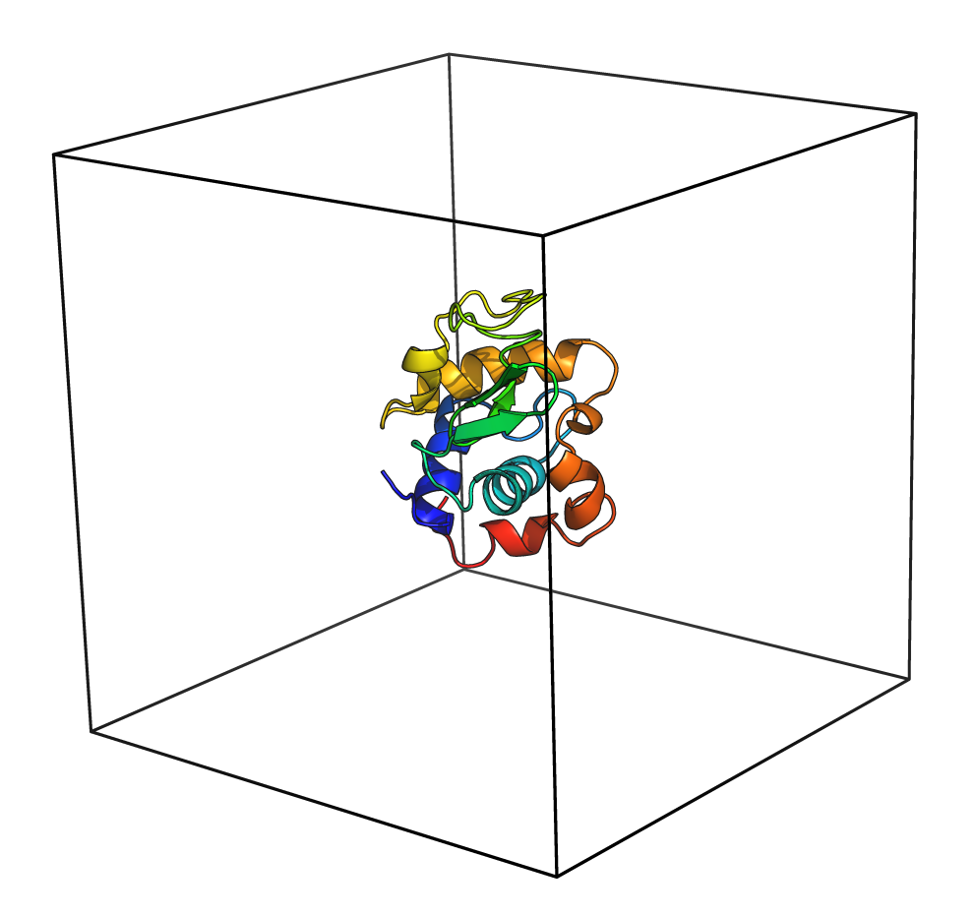
\includegraphics{1AKI_1box}
\caption{The structure of hen egg-white lysozyme in an empty, cubic box following the use of \texttt{editconf}.}
\label{lyso_box_fig}
\end{figure}

Now that the box size and shape have been defined, it is possible to visualize the periodic images of the system that were alluded to above. Such a representation is shown in Figure~\ref{lyso_boxes_fig}.

\begin{figure}[h]
\centering
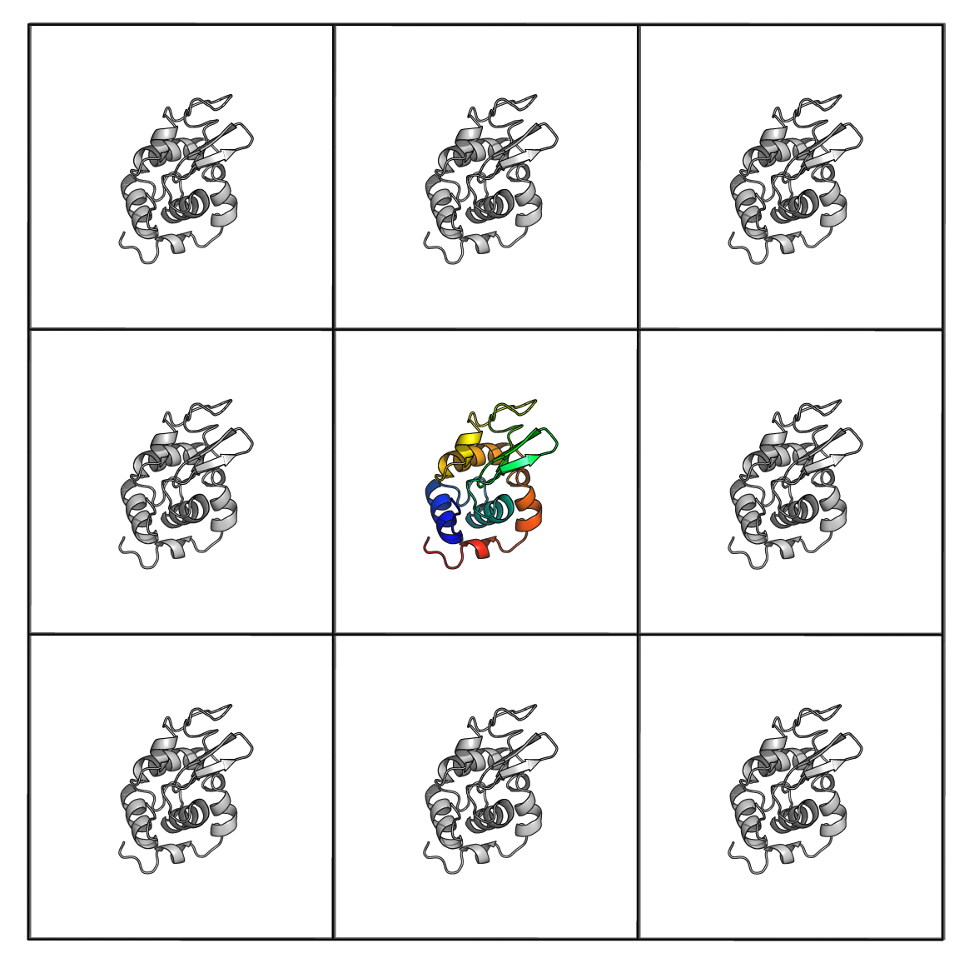
\includegraphics{1AKI_boxes}
\caption{Periodic construction of the central image (with lysozyme colored as a rainbow gradient from blue (N-terminus) to red (C-terminus). Periodic images of the protein are shown in light gray.}
\label{lyso_boxes_fig}
\end{figure}

Having defined a suitable volume around the protein, the system is subsequently filled with water. The program that does this is called \texttt{solvate}. This program relies on the use of a small, pre-equilibrated cubic box of water, which is then placed onto a grid that is evenly distributed through the volume of the \texttt{1AKI\_newbox.gro} coordinate file. Any water molecules with atoms that overlap the protein (or any species already within the box) are deleted.

\begin{lstlisting}
$ gmx solvate -cp 1AKI_newbox.gro -cs spc216.gro -o 1AKI_solv.gro -p topol.top
\end{lstlisting}

The \texttt{solvate} program requires both an input coordinate file for the solute (specified with the \texttt{-cp} option, conventionally the "coordinates of the protein") and the solvent (option \texttt{-cs} for "coordinates of the solvent"). In this example, the empty volume is filled using the \texttt{spc216.gro} coordinate file, which contains 216 water molecules that have been pre-equilibrated using the SPC model~\cite{Berendsen1981}. A common question that new users have is about the availability of coordinates for other 3-point water models such as TIP3P~\cite{Jorgensen1983} and SPC/E~\cite{Berendsen1987} for the purpose of solvation. Simply, distinct files are not necessary, as any coordinate file of 3-point water can serve as a reasonable starting point for such systems. After a short equilibration period (see below, section~\ref{lyso_equil}), the solvent will relax according to the properties of these other models.

Where does the \texttt{spc216.gro} file come from? GROMACS has a database of pre-built coordinate files for 3-, 4-, and 5-point models of water, located in \texttt{\$GMXLIB} (an environment variable that refers to the \texttt{share/gromacs/top} subdirectory of wherever GROMACS is installed on the computer). GROMACS will search in this directory for files specified on the command line before looking in the working directory.

It is important to note the use of the \texttt{-p} option to specify the name of the system topology. Doing so will cause \texttt{solvate} to automatically update the system topology with the number of water molecules it added. If the user does not supply the topology on the command line, updates must be made manually. It is strongly encouraged that users instruct GROMACS programs to do bookkeeping for them, rather than trying to make manual adjustments that can be error-prone.

\subsubsection{Add Ions} \label{lyso_ions}

With the system solvated, the last step in constructing coordinates is to add ions. Biological and {\em in vitro} systems often contain some amount of salt, and it is in the interest of those performing simulations to model relevant conditions as closely as possible. Beyond this point, MD simulations are typically carried out under electroneutral conditions; that is, the system does not carry net charge. Individual molecules (proteins, ions, etc.) may carry a formal charge. This convention reflects typical experimental conditions but there is another point that needs to be mentioned. Electrostatic interactions are most often evaluated using the particle mesh Ewald (PME) method~\cite{Darden1993,Essmann1995}, which requires an electroneutral system. The PME method itself can supply what is known as a "uniform neutralizing plasma," in which an offsetting charge is spread uniformly across the system to neutralize it. For homogeneous systems, this approach is adequate and the addition of explicit ions is not required. However, systems of biological interest are rarely homogeneous, and relying on the neutralizing plasma can result in serious artifacts~\cite{Hub2014}. For this reason, monoatomic ions are typically added within the aqueous solution to counterbalance any net charge from the solute(s) present.

The GROMACS program for adding ions is called \texttt{genion}. It adds ions by replacing molecules in whatever group the user specifies, typically water. To do so, \texttt{genion} needs both coordinate information (to know what coordinates to assign to the added ions) as well as topological information (to know which atoms are connected, therefore defining molecules that are deleted in their entirety). Such information is present in a single file type with the extension \texttt{.tpr}. A \texttt{.tpr} file also contains simulation instructions, which are written in plain-text files with the extension \texttt{.mdp}. In this context, no instructions for performing a simulation are required, but the file format contains everything that is needed. The contents of an \texttt{.mdp} file will be discussed in detail in subsequent sections of this tutorial. To produce a \texttt{.tpr} file, invoke the GROMACS preprocessor, \texttt{grompp}:

\begin{lstlisting}
$ gmx grompp -f ions.mdp -c 1AKI_solv.gro -p topol.top -o ions.tpr
\end{lstlisting}

The \texttt{grompp} program reads in coordinates (\texttt{-c}), topology (\texttt{-p}), and a simulation input file (\texttt{-f}) and produces the \texttt{.tpr} file. For the purpose of adding ions, the \texttt{.mdp} file passed to the \texttt{-f} option can contain any syntactically correct set of options. In this tutorial, a very simple file (\texttt{ions.mdp}) is supplied, to minimize the number of options that must be correctly specified. The \texttt{ions.mdp} file calls for energy minimization but this process is not actually carried out. It is also important to note that a plain cutoff method is specified for electrostatics; doing so is inadvisable for performing a simulation, but \texttt{grompp} will generate a warning if the user attempts to execute a process with PME for a non-neutral system. As counterions have not yet been added to the system, PME should not be specified. Moreover, since this \texttt{.mdp} file is not actually being used for any simulation, it need not specify rigorous simulation methods.

Recall the net charge printed by \texttt{pdb2gmx}, which should be +8. This number means that the protein has a net positive charge at neutral pH, requiring the addition of 8 anions to neutralize it. To do so, execute \texttt{genion} as follows:

\begin{lstlisting}
$ gmx genion -s ions.tpr -o 1AKI_solv_ions.gro -p topol.top -pname NA -nname CL -neutral
\end{lstlisting}

Choose group 13 (SOL) to replace water molecules with ions. Do not choose System or Protein, or any similar group, otherwise the output system will be completed fragmented and unphysical.

\texttt{genion} reads the \texttt{.tpr} file passed to the \texttt{-s} option and outputs (\texttt{-o}) a coordinate file called \texttt{1AKI\_solv\_ions.gro}. It makes changes to the topology (deleting water and adding the requested ions), therefore the use of \texttt{-p} to specify the topology is strongly encouraged. The \texttt{-pname} and \texttt{-nname} specify the residue names of positive and negative ions, respectively. This example does not require the addition of sodium ions (Na\textsuperscript{+}) but is shown for illustrative purposes. The user can specify the number of negative ions to be added with \texttt{-nn}, and if positive ions were needed, they would be specified with \texttt{-np}. Note that the charge on different systems will be different, and in some instances, it is desirable to add a higher salt concentration. To automatically neutralize a system, use the \texttt{-neutral} option, and to set a target concentration for which \texttt{genion} will determine the number of ions to be added (rather than specifying them manually), use \texttt{-conc} with a suitable value (in M).

The final, solvated system will look something like what is shown in Figure~\ref{lyso_solv_ions_fig}. Note that due to the random nature of adding ions with \texttt{genion}, the location of Cl\textsuperscript{$-$} ions will differ in every system.

\begin{figure}[h]
\centering
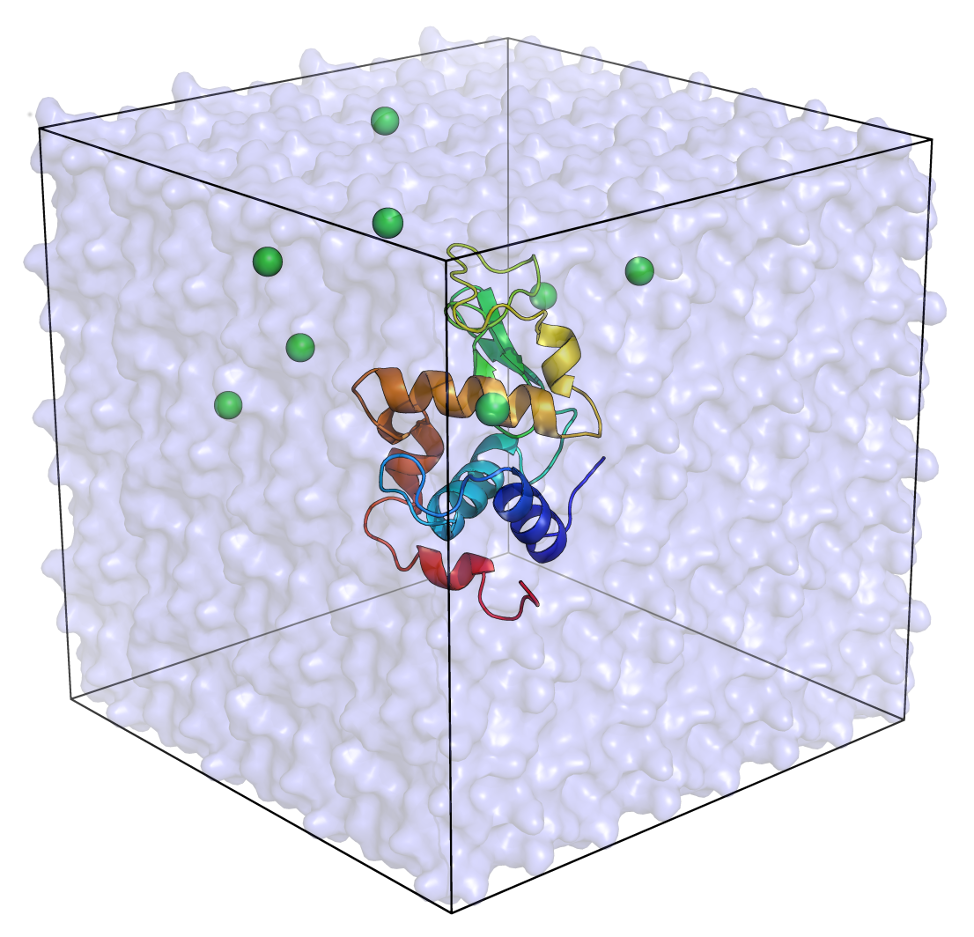
\includegraphics{1AKI_solv_ions}
\caption{Rendering of the final system after solvation and adding ions. Green spheres are Cl\textsuperscript{$-$} ions, whose positions will vary randomly as a result of \texttt{genion}.}
\label{lyso_solv_ions_fig}
\end{figure}

\subsubsection{Energy Minimization} \label{lyso_em}

Before beginning dynamics, it is necessary to relax the solvated system to a low-energy state. Energy minimization is the process that moves the positions of atoms according to the forces acting upon them. In preparing the system, hydrogen atoms were constructed by \texttt{pdb2gmx} in assumed geometries, water molecules were added in a grid around the protein by \texttt{solvate} in a manner that may create suboptimal hydrogen bonding, and ions were added randomly by \texttt{genion} with no regard to nearby atoms with which the charges might clash. As a result, the system must be relaxed to a low-energy state, otherwise any simulation will likely be unstable. It is impossible to know whether or not the system is at its global energy minimum, but this is not necessarily the goal of energy minimization, rather it seeks to find a reasonable starting point for the simulation.

In this section, the contents of the \texttt{.mdp} file will be discussed in depth. Refer to the \texttt{minim.mdp} file, which will be used as the instructions for the energy minimization process. The first section of this input file specifies the parameters for carrying out energy minimization:

\begin{lstlisting}
integrator	= steep
emtol      = 1000.0
emstep     = 0.01
nsteps     = 50000
\end{lstlisting}

These instructions tell the GROMACS program \texttt{mdrun} (discussed below) to use the steepest descents method for energy minimization, and to terminate the process if the magnitude of the potential energy gradient is 1000.0 kJ mol\textsuperscript{-1} nm\textsuperscript{-1} or smaller. The maximum step size along the gradient is 0.01 nm, and a maximum of 50000 steps are allowed. The default value of \texttt{emstep} in GROMACS of 0.01 nm is used, but it is often necessary to use a smaller maximum step ({\em e.g.} 0.002 nm) for systems that have difficulty converging; the smaller step size allows for a more thorough walk over the potential energy surface, whereas a larger step may miss a path to the true minimum. It is also possible to allow the process to go on indefinitely, stopping only when convergence is reached (due to numerical precision or by actually achieving \texttt{emtol}) by setting \texttt{nsteps = -1}. Note that \texttt{emstep} has units of distance, not time. Energy minimization is not a dynamical process; time does not elapse between each step and there are no velocities. Energy minimization steps are expressed in terms of maximum displacement along the vector indicated by the force.

The remainder of the \texttt{.mdp} file contains instructions for how to compute nonbonded interactions:

\begin{lstlisting}
nstlist       = 1
cutoff-scheme = Verlet
ns_type       = grid
coulombtype   = PME
rcoulomb      = 1.0
rvdw          = 1.0
pbc           = xyz
\end{lstlisting}

The value of \texttt{nstlist} controls how many steps (minimization or MD integration) elapse between updating the neighbor list for determining which atoms contribute to the short-range forces. In MD simulations, this value is larger because atoms exchange from the neighbor list in diffusion-limited time, but for energy minimization, it needs to be set to 1 because the configuration may change considerably between each step. The \texttt{cutoff-scheme = Verlet} setting uses a buffered neighbor list, that is, atoms outside the longest cutoff are still tracked to improve energy conservation. Neighbor searching is done by checking atoms in neighboring grids (\texttt{ns\_type = grid}) rather than checking every possible atom (\texttt{ns\_type = simple}). All short-range nonbonded interactions (electrostatics and van der Waals) are truncated at 1.0 nm (\texttt{rcoulomb = 1.0} and \texttt{rvdw= 1.0}), and periodic boundary conditions are applied in all three dimensions (\texttt{pbc = xyz}). The PME method is used to calculate long-range electrostatic forces.

Note that in \texttt{.mdp} files, there is no difference between a hyphen (-) and underscore (\_); hence in the above example, \texttt{ns-type} and \texttt{ns\_type} would be equivalent, as would \texttt{cutoff-scheme} and \texttt{cutoff\_scheme}.

As above, invoke \texttt{grompp} to assemble the instructions for energy minimization (\texttt{-f minim.mdp}), coordinates \\(\texttt{-c 1AKI\_solv\_ions.gro}), and topology (\texttt{-p topol.top}) to create the run input file for energy minimization (\texttt{-o em.tpr}):

\begin{lstlisting}
$ gmx grompp -f minim.mdp -c 1AKI_solv_ions.gro -p topol.top -o em.tpr
\end{lstlisting}

The GROMACS \texttt{mdrun} program is responsible for performing all minimization and dynamics processes. To run energy minimization, use the following syntax:

\begin{lstlisting}
$ gmx mdrun -v -deffnm em
\end{lstlisting}

The \texttt{-v} option invokes "verbose" mode, in which an estimate of time remaining is printed to the screen, along with the current energy minimization step, the step size, potential energy, and maximum force. It is not a required option, and if printed to a file, may result in a large file that is saved to disk. It is, however, instructive to watch the progress of energy minimization to understand what is going on. The \texttt{-deffnm} option defines the base file name for all input and output files and eliminates the need for using individual input and output flags to specify names. 

\texttt{mdrun} requires the \texttt{.tpr} file as its only input, normally passed to the \texttt{-s} flag. \texttt{mdrun} produces several file types, including an ASCII text file with a \texttt{.log} extension, a binary file with all energy values with a \texttt{.edr} extension, and trajectory files with either \texttt{.trr} (full-precision coordinates, velocities, and/or forces) or \texttt{.xtc} (reduced precision coordinates only) extensions. When using \texttt{-deffnm}, these files will be called \texttt{em}, with a corresponding file extension. It is useful to name files in this manner to avoid relying on default file names (\texttt{md.log}, \texttt{ener.edr}, \texttt{traj.trr}, \texttt{traj\_comp.xtc}), which will be the same for any process carried out by \texttt{mdrun}.

When \texttt{mdrun} is done, the user will see something similar to the following:

\begin{lstlisting}[basicstyle=\footnotesize\ttfamily]
Steepest Descents converged to Fmax < 1000 in 726 steps
Potential Energy  = -5.8448769e+05
Maximum force     =  9.6957593e+02 on atom 736
Norm of force     =  2.3290928e+01
\end{lstlisting}

For a system such as this, it is expected that the final potential energy will be a negative value, on the order of 10\textsuperscript{5} - 10\textsuperscript{6} kJ mol\textsuperscript{-1}. Potential energy is an extrinsic quantity, so larger systems will have larger magnitudes. For a solvated protein, the value will be negative, as favorable electrostatic interactions between water molecules dominate the potential energy terms. Smaller systems may even have positive potential energy, arising from the fact that in such cases, the intramolecular bonded terms have a larger magnitude than nonbonded terms. Bonded components of the potential energy function have positive values, by definition. So for small systems, these may prevail and the final, potential energy is positive. Such an outcome is not necessarily an indication that anything is wrong. It would, however, be unusual for a fully solvated protein system such as this one to have a positive potential energy.

The various energy terms saved during energy minimization are stored in the \texttt{em.edr} file, and can be extracted with the \texttt{energy} program. For example, to extract the potential energy of a system as a function of energy minimization step:

\begin{lstlisting}
$ gmx energy -f em.edr -o potential.xvg
\end{lstlisting}

By default, GROMACS analysis programs write output formatted for use with the XmGrace plotting program, though this formatting can be changed with the \texttt{-xvgr} option. The output \texttt{potential.xvg} file can be plotted to produce Figure~\ref{lyso_em_fig}.

\begin{figure}[h]
\centering
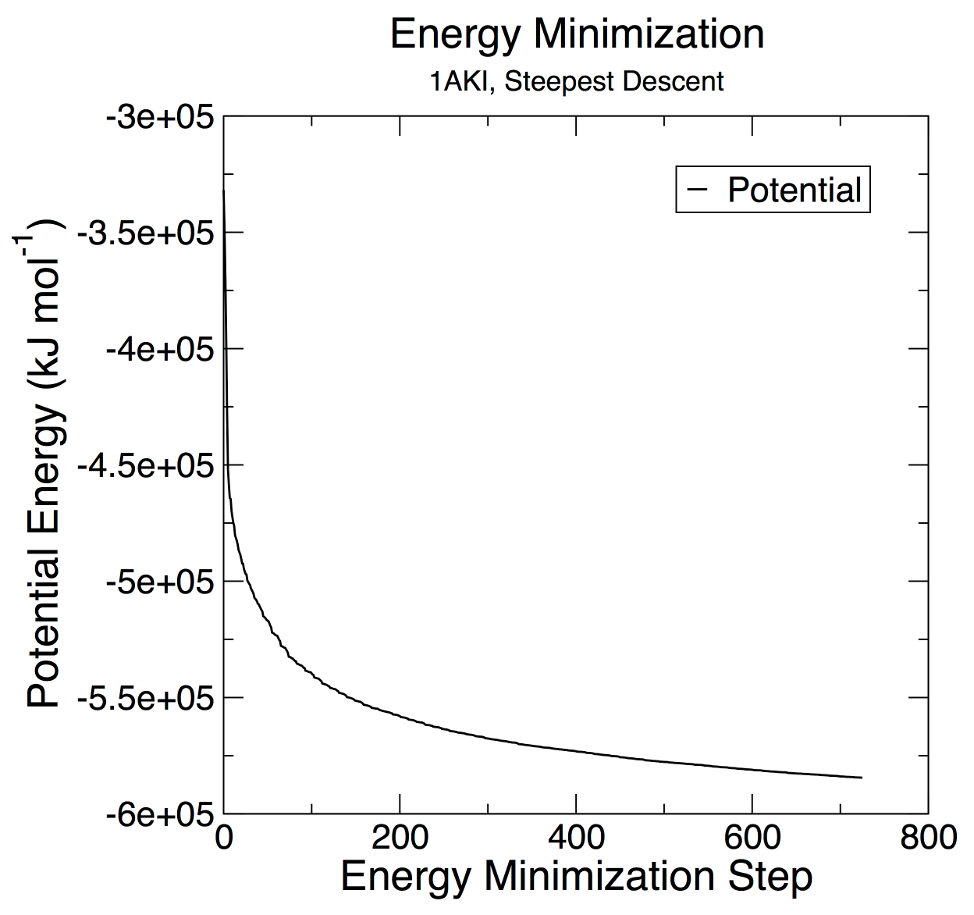
\includegraphics{plot_lyso_em_potential}
\caption{Potential energy of the solvated lysozyme system as a function of energy minimization step.}
\label{lyso_em_fig}
\end{figure}

The solvated system is now at a reasonable energy minimum. Note that the steepest descents method is very efficient but also may have difficulty finding a true energy minimum. The settings used in this tutorial are fairly permissive but work reasonably well for most similar systems. There are applications, however, that require more exhaustive energy minimization (for instance, free energy calculations such as those in section~\ref{fes}), either through multiple rounds of minimization with different algorithms that may more carefully sample energy minima, or with stricter convergence criteria.

It is also important to note that the large changes in potential energy are often confusing to new users. During dynamics, it is expected that energy will be conserved, but the purpose of energy minimization is to change the configuration of the system in a manner that leads to a decrease in energy. As such, obtaining an average energy during energy minimization is not a useful metric, nor is any examination of energy conservation.

\subsubsection{Equilibration} \label{lyso_equil}

Following energy minimization, the system is now ready for the start of dynamics. Equilibration is carried out to obtain a stable thermodynamic ensemble for whatever conditions are desired. Most biomolecular simulations are carried out under a canonical (NVT) ensemble, in which the number of particles (N), volume (V), and temperature (T) of the system are conserved, or an isothermal-isobaric (NPT) ensemble, in which the number of particles (N), pressure (P), and temperature (T) are conserved. There are other statistical mechanical ensembles that can be employed, but this tutorial will focus on those that are most relevant to biomolecular systems. Before carrying out a simulation under a given ensemble, the system must be equilibrated under the same conditions. For this tutorial, the production MD simulation will be carried out under an NPT ensemble. It is possible to simply initiate an equilibration simulation under the same conditions, but it is often more robust to first equilibrate the temperature of the system under an NVT ensemble before applying a barostat to control the temperature. The simultaneous combination of velocity generation and coordinate scaling under the influence of the barostat can introduce instabilities in a system that may be far from equilibrium.

It is also important to note that rather than initiating the simulation at the desired temperature, it is also possible to slowly warm the system up. This technique will not be applied in this tutorial, as there is some debate as to whether or not it is necessary in most cases. Interested readers are directed to the GROMACS manual section on "simulated annealing" for information on how this process is carried out in GROMACS.

To initialize dynamics, velocities are generated by \texttt{grompp} and written to the \texttt{.tpr} file. The following settings in the \texttt{nvt.mdp} file control the generation of velocities:

\begin{lstlisting}
gen_vel                 = yes
gen_temp                = 300
gen_seed                = -1
\end{lstlisting}

A new concept is the application of position restraints. A restraint is a biasing potential that is applied to selected atoms to disfavor motion. It should be noted that position restraints do not prevent motion, rather they penalize it. Position restraints are typically applied to solute non-hydrogen atoms during equilibration to prevent deformations that could be induced by the random nature of the starting velocities and subsequent collisions between the solute and solvent. Position restraints are specified with the following keyword in the \texttt{nvt.mdp} file:

\begin{lstlisting}
define                  = -DPOSRES
\end{lstlisting}

Recall the generation of the \texttt{posre.itp} file by \texttt{pdb2gmx} in section~\ref{lyso_top}, which is only invoked as part of an \texttt{\#ifdef} block in \texttt{topol.top}. This construct means restraints are only applied when the user wants them, with invocation being dependent upon the use of the \texttt{define} keyword in the \texttt{.mdp} file. The presence of \texttt{define = -DPOSRES} means that the \texttt{\#ifdef POSRES} condition is evaluated as true by \texttt{grompp} and the position restraint topology (\texttt{posre.itp}) is applied to the system. Note that the general syntax of \texttt{\#ifdef KEYWORD} and \texttt{define = -DKEYWORD}; failing to prefix the keyword with \texttt{-D} will not lead to any error, but the \texttt{\#ifdef} condition will not be matched.

Some of the settings in the \texttt{.mdp} file are the same as in energy minimization and will not be repeated here. New settings that are introduced during NVT are:

\begin{lstlisting}
integrator              = md
nsteps                  = 50000
dt                      = 0.002
\end{lstlisting}

The above lines specify that this process is an MD simulation, and the \texttt{md} setting specifies the leap-frog integrator in GROMACS. A total of 50,000 integration steps will be performed, and each step corresponds to an integration time step, $\delta$t, of 0.002 ps, or 2 fs. The simulation will therefore last for 100 ps (50,000 steps $\times$ 0.002 ps per step).

Output is specified in the next section of \texttt{nvt.mdp}:

\begin{lstlisting}
nstxout                 = 500
nstvout                 = 500
nstenergy               = 500
nstlog                  = 500
\end{lstlisting}

The \texttt{nstxout} and \texttt{nstvout} settings control the interval of time steps between writing coordinates (x) and velocities (v) to the trajectory (\texttt{.trr}) file. With these settings, coordinates and velocities are saved every 1 ps. Similarly, energy terms are written to the \texttt{.edr} file (\texttt{nstenergy}) and \texttt{.log} file (\texttt{nstlog}) at the same interval.

Bond constraints are applied to allow for the 2-fs integration time step specified above. The value of $\delta$t is limited by the fastest vibrational modes in the system, which are typically bonds to hydrogen atoms. As these bonds will rarely exist in excited states, it is reasonable to model them as rigid, replacing the harmonic oscillator term with a holonomic constraint. Doing so allows the value of $\delta$t to be increased from roughly 0.5 fs up to 2 fs for typical dynamics runs. In the \texttt{.mdp} file, the relevant settings are:

\begin{lstlisting}
continuation            = no
constraint_algorithm    = lincs
constraints             = h-bonds
lincs_iter              = 1
lincs_order             = 4
\end{lstlisting}

The \texttt{continuation} keyword tells \texttt{mdrun} that the coordinates are not the output of a previously constrained simulation, so the constraints need to be solved at the first time step. The method for applying constraints is LINCS, the Linear Constraint Solver~\cite{Hess1997,Hess2008b}. Constraints are applied to bonds to hydrogen atoms \texttt{constraints = h-bonds}, and the remaining settings are the default LINCS parameters for accuracy of the constraint equations. It is important to note that "constraints" and "restraints" are different. As described above, a restraint is a biasing potential that disfavors motion, whereas a constraint is used to fix a distance or angle in a simulation. Older literature often uses these terms interchangeably, but in modern simulation practice, these two terms have distinct meaning.

The next relevant section is related to nonbonded interactions, which were described above in section~\ref{lyso_em}. After the nonbonded settings are the keywords related to temperature control:

\begin{lstlisting}
tcoupl              = V-rescale
tc-grps             = Protein Non-Protein
tau_t               = 0.1     0.1
ref_t               = 300     300
\end{lstlisting}

The \texttt{tcoupl} keyword specifies the algorithm that is used for temperature coupling, also known as the thermostat. In this example, the velocity rescaling method of Bussi et al. is applied~\cite{Bussi2007}. Another thermostat commonly applied during equilibration is the weak coupling method of Berendsen et al.~\cite{Berendsen1984} (specified with \texttt{tcoupl = berendsen} in the \texttt{.mdp} file). The Berendsen weak coupling method has fallen out of favor, as it has been demonstrated that it does not sample a correct canonical velocity distribution~\cite{Bussi2007}. The Bussi velocity rescaling method, however, does sample a correct velocity distribution, and has the same advantages as the Berendsen method in that it quickly relaxes the system to the target temperature, making it practical and efficient for use in both equilibration and production MD simulations. The \texttt{tc-grps} keyword specifies which groups of atoms are coupled to the specified thermostat. All atoms should be coupled, but they can be separated into different groups. Strictly speaking, any separation of atoms into different groups violates the Equipartition Theorem, in that thermal energy can flow into and out of the thermal reservoir (thermostat) independently between the different groups, rather than being exchanged between the atoms in the system. The practice of coupling solute and solvent atoms separately arises from the "hot solvent/cold solute" problem in MD simulations~\cite{Lingenheil2008}, in which the solvent heats while the solute cools, due to a host of factors related to approximations made in MD integration. Here, the protein and all other non-protein atoms (water and ions) are coupled to separate thermostats at 300 K, with a coupling time ($\tau_{T}$) of 0.1 ps, which reflects rather tight regulation, which is appropriate for equilibration.

Create the NVT equilibration \texttt{.tpr} file with \texttt{grompp}:

\begin{lstlisting}
$ gmx grompp -f nvt.mdp -c em.gro -r em.gro -p topol.top -o nvt.tpr
\end{lstlisting}

The command-line options to \texttt{grompp} are largely the same as those used above for energy minimization, but there is one addition, the \texttt{-r} flag. This option specifies the name of a coordinate file that is used as the origin for the position restraint biasing potential. That is, this coordinate file contains the reference positions (hence \texttt{-r}) at which the biasing potential on the atoms would be zero. In previous versions of GROMACS, this option was not mandatory, but in the 2018 version, it is required to prevent users from incorrectly specifying the origin of their biasing potentials. In most cases, however, the coordinates passed to \texttt{-c} and \texttt{-r} will be the same. There are advanced use cases in which different coordinate files will be used, but they are beyond the scope of this tutorial.

Perform NVT equilibration by invoking \texttt{mdrun}:

\begin{lstlisting}
$ gmx mdrun -deffnm nvt
\end{lstlisting}

After the run, analyze the temperature time series to verify that the target temperature (300 K) was achieved and maintained, using the \texttt{energy} program. At the prompt, type \texttt{16 0}, then Enter. Group 16 is the temperature time series, and 0 terminates input to \texttt{energy}.

\begin{lstlisting}
$ gmx energy -f nvt.edr -o temperature.xvg
\end{lstlisting}

The time series of temperature during NVT is shown in Figure~\ref{lyso_nvt_temp_fig}.

\begin{figure}[h]
\centering
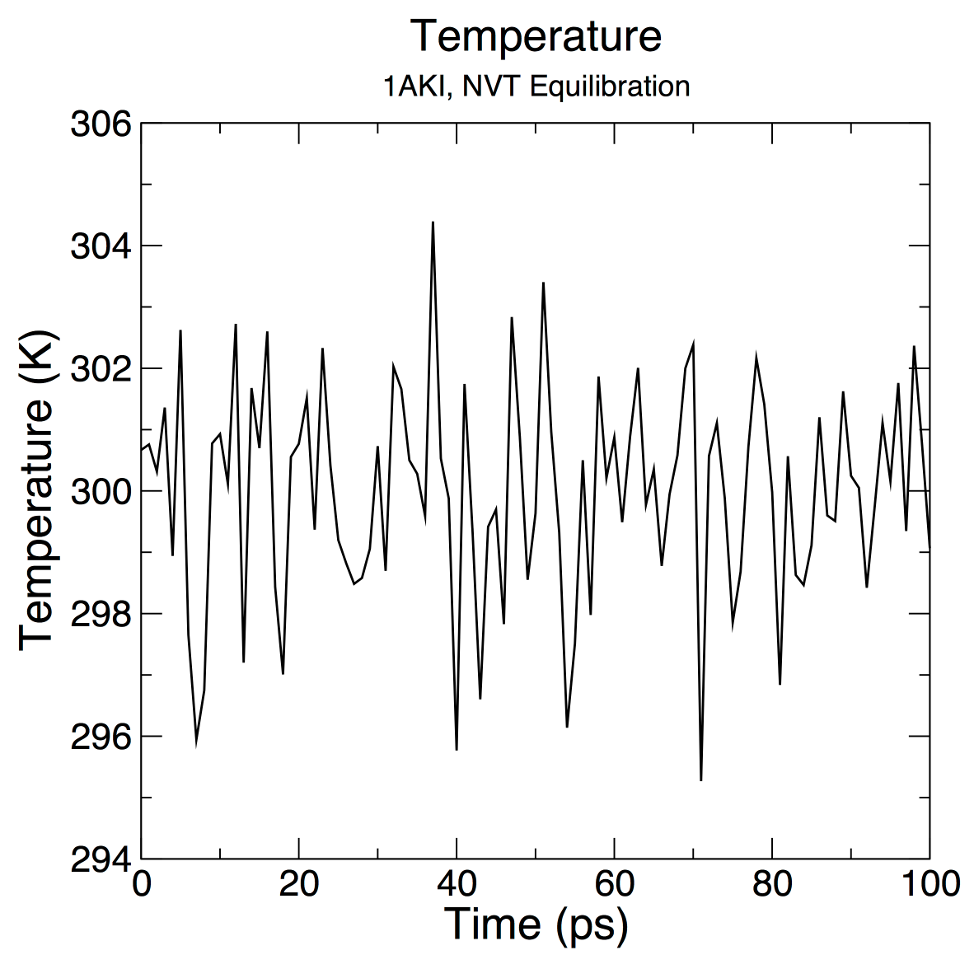
\includegraphics{plot_lyso_nvt_temperature}
\caption{Temperature of the solvated lysozyme system over time during NVT equilibration.}
\label{lyso_nvt_temp_fig}
\end{figure}

As it is ultimately desirable to conduct the production MD simulation under NPT conditions (reflecting typical laboratory conditions), equilibration is continued under an NPT ensemble. Position restraints are maintained on the protein non-hydrogen atoms. New settings in the \texttt{.mdp} file related to pressure coupling are as follows:

\begin{lstlisting}
pcoupl                  = Parrinello-Rahman
pcoupltype              = isotropic
tau_p                   = 2.0
ref_p                   = 1.0
compressibility         = 4.5e-5
refcoord_scaling        = com
\end{lstlisting}

The equilibration protocol utilizes a barostat method proposed by Parrinello and Rahman~\cite{Parrinello1981}, and later modified by Nos\'e and Klein~\cite{Nose1983}. As with thermostats explained in the NVT equilibration step, barostats require a reference pressure (\texttt{ref\_p}) and a period of time over which the pressure of the system is allowed to relax towards the target (\texttt{tau\_p}). The \texttt{pcoupltype} keyword controls the deformation of the box in all three dimensions. For a homogenous system such as the one constructed here, it is appropriate to scale all box vectors uniformly. Such scaling is achieved with \texttt{isotropic} pressure coupling. GROMACS has options for semi-isotropic, with $x$ and $y$ coupled together, $z$ coupled independently, as will be used in the membrane protein tutorial (see Section~\ref{kalp}). Anisotropic coupling allows all dimensions (including diagonal elements of the box) to be scaled separately (useful for crystalline materials and solid phases). The \texttt{compressibility} setting controls the speed of the response of the barostat and is, by default, set to the isothermal compressibility of water (4.5 $\times$ 10\textsuperscript{-5} bar\textsuperscript{-1}). 

The \texttt{refcoord\_scaling} setting is often confusing for new users. Pressure is scaled by actually scaling atomic coordinates as a function of increases or decreases in box size. The reference coordinates (see NVT equilibration above) set the origin of the position restrain biasing potential. If the reference coordinates are not similarly scaled, the forces applied due to the restraints will accumulate and become artificial as the updated coordinates drift slightly and are scaled, while the reference coordinates remain fixed. Reference coordinates can be scaled either based on the center-of-mass (COM) of the restrained molecule(s) or by individual atoms. In principle, either approach works sufficiently well for equilibration, but scaling relative to the COM of the restrained molecule(s) is often somewhat more numerically stable, especially for systems that are not necessarily at thermodynamic equilibrium.

An additional difference in the \texttt{npt.mdp} file is the treatment of bonds. The \texttt{continuation} keyword is set to a value of \texttt{yes}, indicating that this simulation run is the continuation of a previous run in which constraints were applied. To preserve continuity, the constraints should not be re-solved, and the input coordinates should be assumed to satisfy the constraint algorithm being applied.

Prepare the run input file (\texttt{.tpr}) again using \texttt{grompp}. Note here that the checkpoint file from NVT equilibration (\texttt{nvt.cpt}) is passed to the \texttt{grompp -t} option. The checkpoint file contains a complete description of the thermodynamic state of the system, in high precision. To exactly continue a simulation, the checkpoint file must be passed to \texttt{grompp}. If it is omitted, information regarding velocities, thermostat variables, and high-precision coordinates will be lost. The checkpoint file is an essential component of proper continuation of MD simulations.

\begin{lstlisting}
$ gmx grompp -f npt.mdp -c nvt.gro -r nvt.gro -t nvt.cpt -p topol.top -o npt.tpr
\end{lstlisting}

As before, execute \texttt{mdrun} to perform NPT equilibration:

\begin{lstlisting}
$ gmx mdrun -deffnm npt
\end{lstlisting}

After the run has concluded, again use the \texttt{energy} program, in this case to extract the pressure time series. Enter 18 to select Pressure, and 0 to terminate input to \texttt{energy}:

\begin{lstlisting}
$ gmx energy -f npt.edr -o pressure.xvg
\end{lstlisting}

The pressure time series is plotted in Figure~\ref{lyso_npt_pres_fig}. The screen output also indicates that the average pressure was 7.5 $\pm$ 160.5 bar. The target value was 1 bar. This discrepancy is often a source of concern for new users. Consider, however, the large error bar associated with the time series, and the wide range of pressure values sampled during the simulation (Figure~\ref{lyso_npt_pres_fig}). Pressure is a quantity that fluctuates wildly in a microscopic system. As a result, instantaneous values are going to vary considerably, and average values may not correspond exactly to the desired target value. However, given the huge standard deviation of pressure during NPT equilibration (160.5 bar), the average obtained during the simulation (7.5 bar) is statistically indistinguishable from the target of 1 bar. It is possible to extend the NPT equilibration phase for additional time in an attempt to obtain better agreement, but it is not necessary to do so. The existing agreement is sufficient.

\begin{figure}[h]
\centering
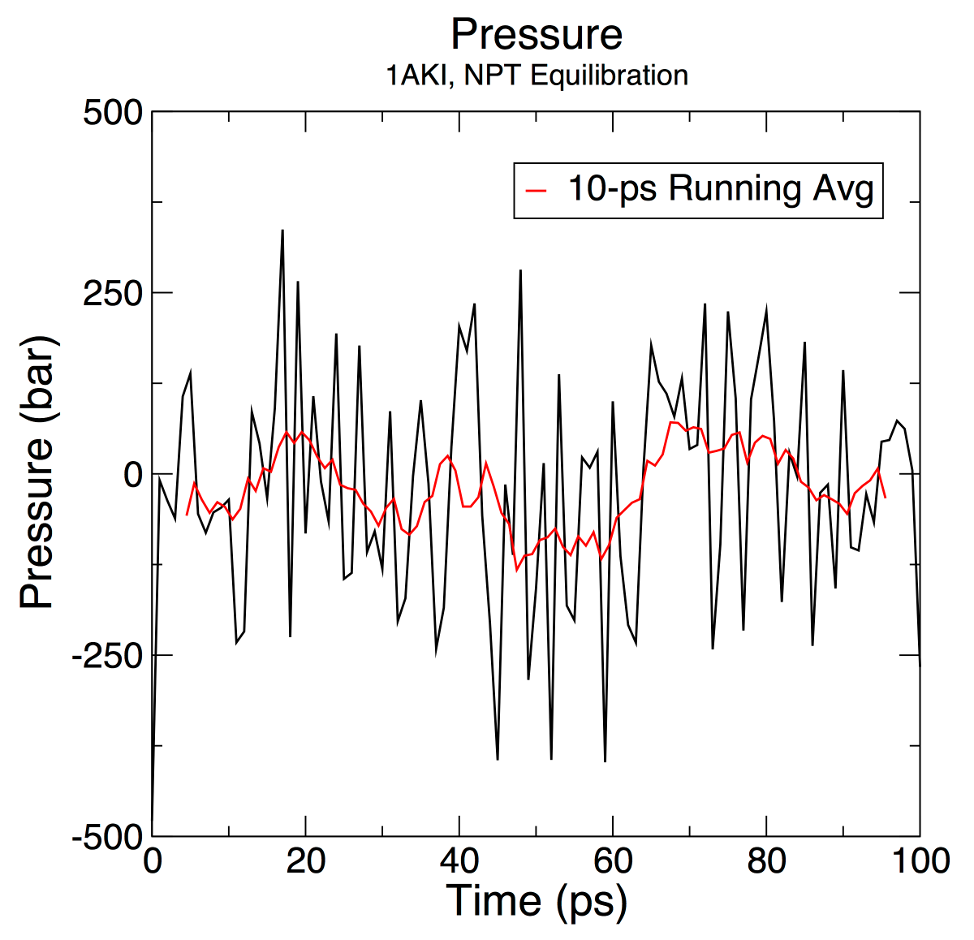
\includegraphics{plot_lyso_npt_pressure}
\caption{Pressure of the solvated lysozyme system over time during NPT equilibration.}
\label{lyso_npt_pres_fig}
\end{figure}

An additional indicator of the convergence of NPT equilibration is the density of the system. Density is less prone to the fluctuations observed in the instantaneous pressure values. Again, use the \texttt{energy} program to extract the density time series from the \texttt{npt.edr} file, choosing 24 for density and 0 to terminate input:

\begin{lstlisting}
$ gmx energy -f npt.edr -o density.xvg
\end{lstlisting}

The density time series is shown in Figure~\ref{lyso_npt_dens_fig}. The average value from NPT equilibration is 1019 $\pm$ 3 kg m\textsuperscript{-3}. Note that this value is about two percent higher than the expected value for bulk SPC/E water (998 kg m\textsuperscript{-3})~\cite{Berendsen1987}. Such an outcome is not unusual, as the system contains a protein and ions, therefore its density will not be exactly equivalent to that of pure water.

\begin{figure}[h]
\centering
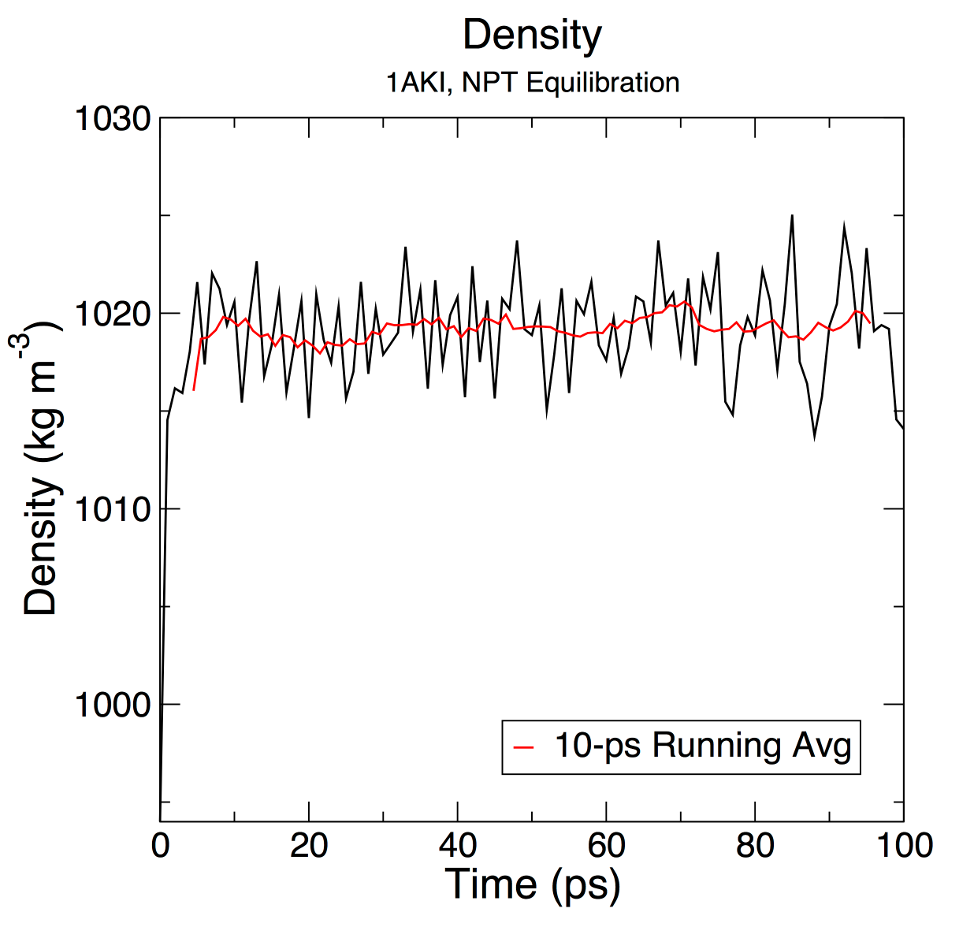
\includegraphics{plot_lyso_npt_density}
\caption{Density of the solvated lysozyme system over time during NPT equilibration.}
\label{lyso_npt_dens_fig}
\end{figure}

Since the density is essentially constant over the duration of NPT equilibration, it is reasonable to conclude that the system is adequately equilibrated and unrestrained simulations can be initiated.

\subsubsection{Production MD Simulation} \label{lyso_md}

At this point, the solvent has relaxed around the protein and the system is equilibrated under the desired statistical mechanical ensemble, NPT. Following equilibration, position restraints are removed from the protein and the simulation proceeds in an unbiased manner. As such, this phase of the MD simulation is often referred to as "unrestrained MD" or "production MD," the latter owing to the fact that trajectory data that are being collected are now considered useful for answering the scientific question(s) at hand.

Production MD proceeds like any other process carried out thus far, with the generation of a \texttt{.tpr} input file with \texttt{grompp}, providing the coordinates and checkpoint file from NPT equilibration to ensure an exact continuation:

\begin{lstlisting}
$ gmx grompp -f md.mdp -c npt.gro -t npt.cpt -p topol.top -o md_0_1.tpr
\end{lstlisting}

Note that in this \texttt{grompp} command, there is no use of \texttt{-r}, as no restraints are being applied. The \texttt{.mdp} settings are the same as during NPT equilibration, except no restraints are specified and the run is being carried out for 500,000 steps, corresponding to 1 ns (500,000 steps $\times$ 0.002 ps per step = 1000 ps = 1 ns).

As before, it is useful to name files in accordance with the time interval and process being simulated. Here, the user will perform a 1-ns, unrestrained MD simulation, starting from t = 0 ns (equilibration time is not counted) and proceeding to t = 1 ns, hence the base file name of \texttt{md\_0\_1}. To run the simulation, invoke \texttt{mdrun}:

\begin{lstlisting}
$ gmx mdrun -deffnm md_0_1
\end{lstlisting}

\subsubsection{Data Analysis} \label{lyso_ana}

Data analysis is the most difficult aspect of carrying out an MD simulation. It is generally advisable to plan appropriate analyses before initiating the simulation to ensure that the simulation is designed in such a way as to produce useful data that answer the scientific question(s) at hand. One should not simply execute a simulation and hope that something interesting will happen that will reveal itself in time. This tutorial cannot possibly cover all analysis methods, nor should the simple tasks here be considered required for analyzing any given MD simulation. In this tutorial, the user will conduct several basic analyses that reflect typical syntax of running various GROMACS analysis routines. Beyond being a fast MD engine, GROMACS comes pre-packaged with numerous analysis programs, facilitating the collection and processing of data.

The first step in analysis is to remove the influence of PBC that were applied during the simulation, a process often referred to as "re-imaging" or "re-wrapping." As a consequence of PBC, molecules often appear "broken" in trajectory frames, or may appear to be "outside" the unit cell. Neither is actually true. Molecules are always intact according to the topology of the system, but may be represented in a manner such that part of a molecule is at one "side" or "corner" of the box, with the remainder elsewhere. This outcome is a result of the fact that visualization convenience is irrelevant to \texttt{mdrun} in its physical calculation. Rather than wasting time re-wrapping molecules to make them appear "whole" during the run, \texttt{mdrun} writes "broken" molecules that must later be fixed, if desired. As molecules diffuse through the system, it may appear that some molecules ({\em e.g.} the protein) "leave" the box or appear "outside" of it. This is not the case; there is no such thing as "outside" an infinite system.

The GROMACS program that applies coordinate manipulations to account for periodicity effects is called \texttt{trjconv} ("trajectory converter") and it serves a number of functions. Beyond accounting for PBC effects, it can be used to convert file formats or save a subset of atoms from the system. In this case, only a simple invocation of \texttt{trjconv} is necessary, to simultaneously make "broken" molecules appear whole and to center the protein in the unit cell. These processes can be done in a single command:

\begin{lstlisting}
$ gmx trjconv -s md_0_1.tpr -f md_0_1.xtc -o md_0_1_noPBC.xtc -pbc mol -center
\end{lstlisting}

The user is prompted for two selections. The first requires a choice of which group to center in the unit cell. Choose group 1 (Protein). The second prompt asks the user to choose which group should be output in the modified trajectory. For simplicity, choose group 0 (System).

Additional manipulations can be applied, such as rotational and translational fitting to produce a smoother visualization of the trajectory. Such fitting relies on a least-squares fit to a reference structure in the \texttt{.tpr} file. For the purposes of this tutorial, no such fitting will be applied, but interested readers are referred to the \texttt{-fit} option of \texttt{trjconv} and associated options. Note that one should not simultaneously use \texttt{-fit} and \texttt{-pbc}, as they are mathematically incompatible. Correct periodicity effects first, then deal with rotational and/or translational fitting.

At this point, the user should visualize the trajectory using programs like VMD~\cite{Humphrey1996}. Watching the progression of the trajectory is the most important part of analysis. Though GROMACS has many built-in analysis routines, the user will not know {\em a priori} everything that will happen during the MD simulation. Animating the trajectory can also be useful for determining if the \texttt{trjconv} treatment was appropriate. Many GROMACS programs are not PBC-aware, meaning if the user does not properly re-image the trajectory to account for PBC effects, analysis will be incorrect, particularly in the case of structure-related properties like those discussed here.

If one is interested in quantifying how much the protein structure changed over the course of the simulation, the root-mean-square deviation (RMSD) can be computed. RMSD is calculated following a least-squares fit to the reference structure and is plotted as a function of time. The GROMACS program that computes RMSD is called \texttt{rms}. It reads the reference coordinates, masses, and topology from the \texttt{.tpr} file passed to \texttt{-s} and computes the RMSD for each frame found in the trajectory passed to \texttt{-f}. Typically, the RMSD of a protein is calculated for its backbone (N, C\textsubscript{$\alpha$}, C) or "main chain" (N, C\textsubscript{$\alpha$}, C, O) atoms rather than the entire structure. Flexible side chains may have large RMSD that do not actually reflect meaningful structural changes. To calculate the RMSD of the protein backbone with respect to the equilibrated coordinates, invoke \texttt{rms} as follows:

\begin{lstlisting}
$ gmx rms -s md_0_1.tpr -f md_0_1_noPBC.xtc -o rmsd.xvg -tu ns
\end{lstlisting}

When prompted, choose group 4 (Backbone) for both the group for fitting and the group for output. The RMSD thus reflects the net change in backbone configuration after accounting for global rotation and translation.

It may also be of interest to calculate the RMSD with respect to some other structure, such as a specific frame of interest or the crystal structure rather than the equilibrated (t = 0 ns) coordinates. To compute the RMSD with respect to the crystal structure, provide \texttt{rms} with the \texttt{em.tpr} file, which was the input to energy minimization. The coordinates of the protein contained therein are the crystal structure with the hydrogen atoms added by \texttt{pdb2gmx}. Invoke \texttt{rms} again:

\begin{lstlisting}
$ gmx rms -s em.tpr -f md_0_1_noPBC.xtc -o rmsd_xtal.xvg -tu ns
\end{lstlisting}

As before, choose group 4 (Backbone) for both the group for fitting and the group for output. The two resulting RMSD time series can be plotted together, as shown in Figure~\ref{lyso_md_rmsd_fig}.

\begin{figure}[h]
\centering
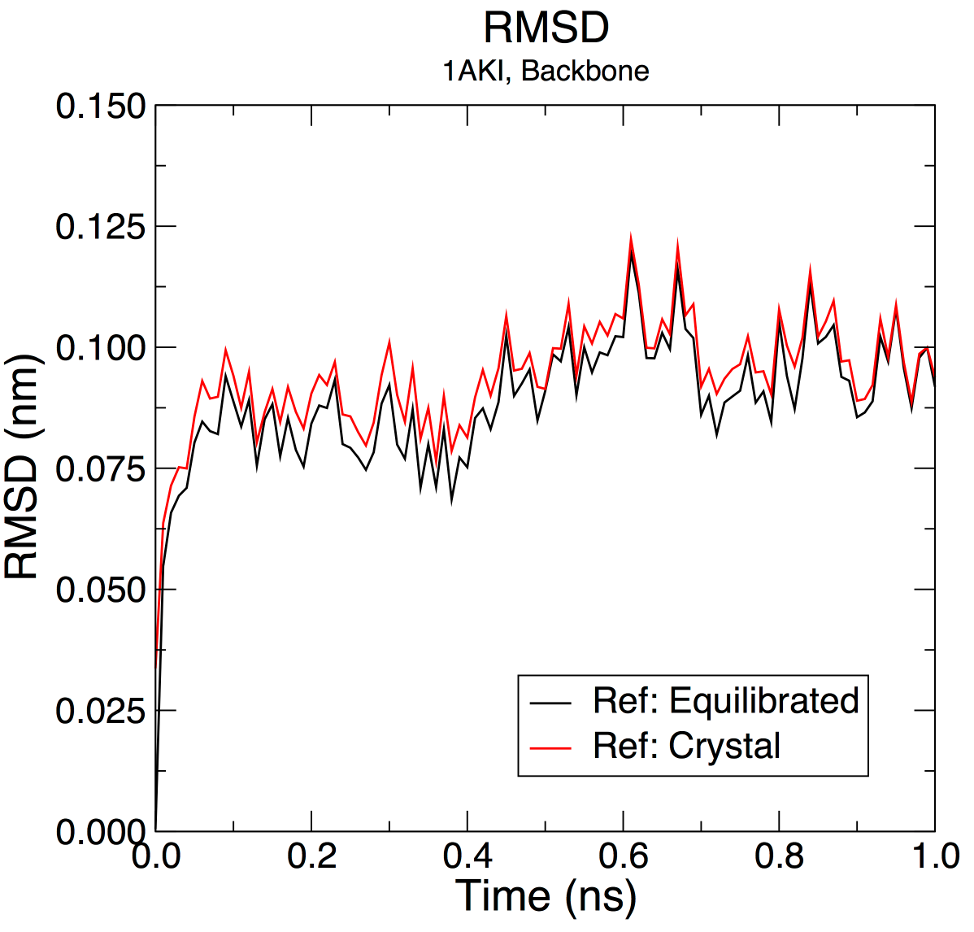
\includegraphics{plot_lyso_md_rmsd}
\caption{RMSD of the lysozyme backbone atoms during the production MD simulation following least-squares fitting to the indicated reference structures.}
\label{lyso_md_rmsd_fig}
\end{figure}

The RMSD values with respect to the crystal structure and equilibrated system are not identical, with the RMSD to the crystal reference being systematically higher than the RMSD to the equilibrated structure. This outcome is not unexpected. Though restraints were applied during equilibration, it is not guaranteed that the protein will not move. Instead, it moves slightly but overall, its conformation is maintained. After about 0.5 ns, the RMSD levels off around 0.1 nm (1~\AA), which is quite small and suggests the protein is very stable. It is appropriate to use this space to dispel several common misconceptions about RMSD. First, it is a degenerate metric, meaning a single value can have multiple interpretations (mathematical solutions), and as such on its own, RMSD is not very useful. Second, one cannot say that a simulation has converged simply based on RMSD, due to the first point $-$ a structure can still be changing considerably from its starting structure even if the RMSD has largely plateaued. Therefore, one should never terminate a simulation, believing it to be "stable" or "converged" simply by looking at RMSD.

As a final example of analysis, calculate the radius of gyration (R\textsubscript{g}) of lysozyme over time with the GROMACS \texttt{gyrate} program. This quantity is not particularly useful for systems of well-folded proteins, as it is a measure of compactness, a quantity expected to be largely constant for a protein with stable tertiary structure. Calculating R\textsubscript{g} demonstrates an advanced capability of GROMACS. Invoke \texttt{gyrate} as follows:

\begin{lstlisting}
$ gmx gyrate -s md_0_1.tpr -f md_0_1_noPBC.xtc -o gyrate.xvg
\end{lstlisting}

\begin{figure}[h]
\centering
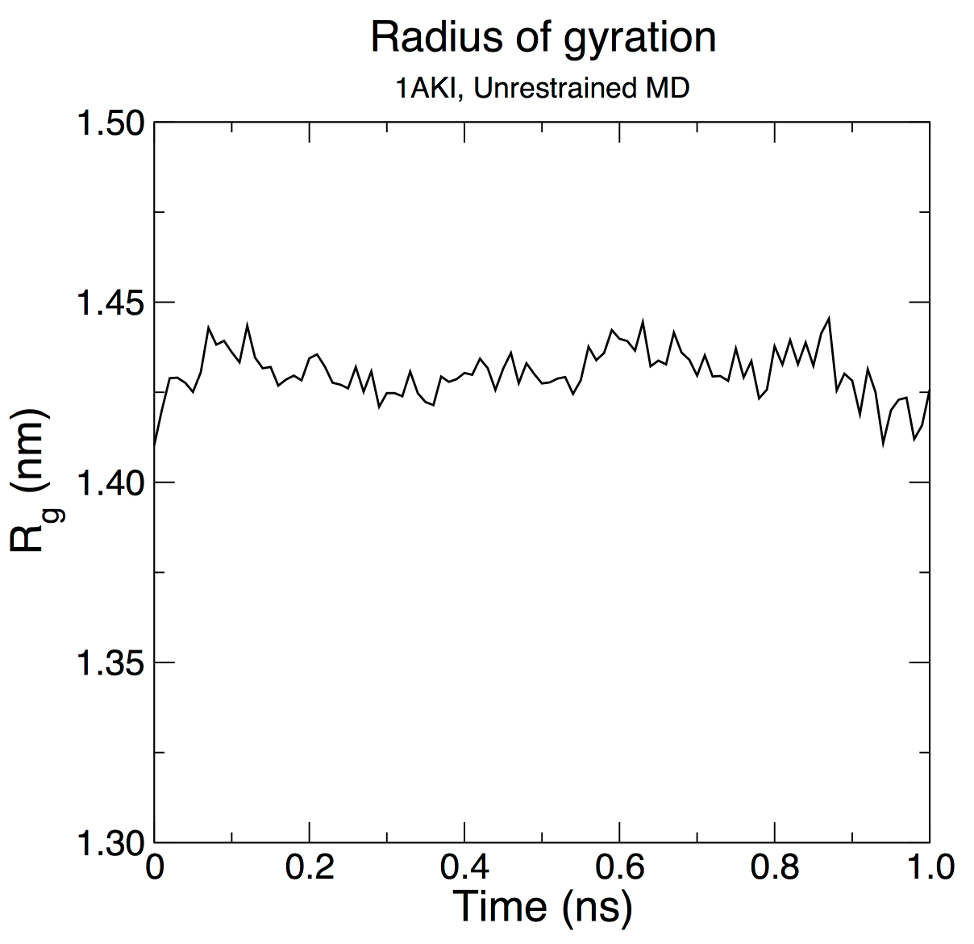
\includegraphics{plot_lyso_md_rg}
\caption{Radius of gyration of lysozyme during the production MD simulation.}
\label{lyso_md_rg_fig}
\end{figure}

The R\textsubscript{g} time series is shown in Figure~\ref{lyso_md_rg_fig}. This quantity is similarly stable over this short simulation, which is expected given the stable fold of lysozyme and the very short nature of the simulation. Large structural changes are not expected within 1 ns for any protein.

\subsubsection{Summary and Review of Objectives} \label{lyso_summary}

Through this tutorial, the user has been guided through the construction of a solvated protein system, including neutralizing counterions. To review, the objectives for this tutorial were as follows:

\begin{enumerate}
	\item Understand the content of a GROMACS system topology
	\item Carry out basic steps of setting up a periodic system, including solvation and adding ions
	\item Identify keywords and typical settings in \texttt{.mdp} input files
	\item Control position restraints and topology directives via \texttt{.mdp} settings
	\item Determine the appropriate algorithms for energy-\\minimizing and equilibrating a biomolecular system and performing a production MD simulation
\end{enumerate}

The first step in the process was the generation of a topology for the protein, to which solvent and ions were added to describe the entire system. The topology contains a listing of the atomic properties, connectivity, and all relevant bonded interactions in the system, as well as topology directives such as \texttt{\#include} to provide additional parameters or define species like water and ions, and \texttt{\#ifdef...\#endif} blocks that allow for selective application of parameters or restraints. Following processing of the protein by \texttt{pdb2gmx}, water was added to a cubic volume with \texttt{solvate} and ions added by \texttt{genion}. The system was energy-minimized with an efficient algorithm, steepest descents, and equilibrated under NVT and NPT ensembles. Recall the practical considerations for thermostat and barostat settings, including the use of a thermostat that properly samples an NVT distribution of kinetic energies. The tutorial concluded with rudimentary analysis that illustrates the basic syntax of GROMACS analysis tools.



%%%%%%%%% TUTORIAL 2 %%%%%%%%%
\subsection{Tutorial 2: KALP\textsubscript{15} in DPPC} \label{kalp}

\begin{figure}[H]
\centering
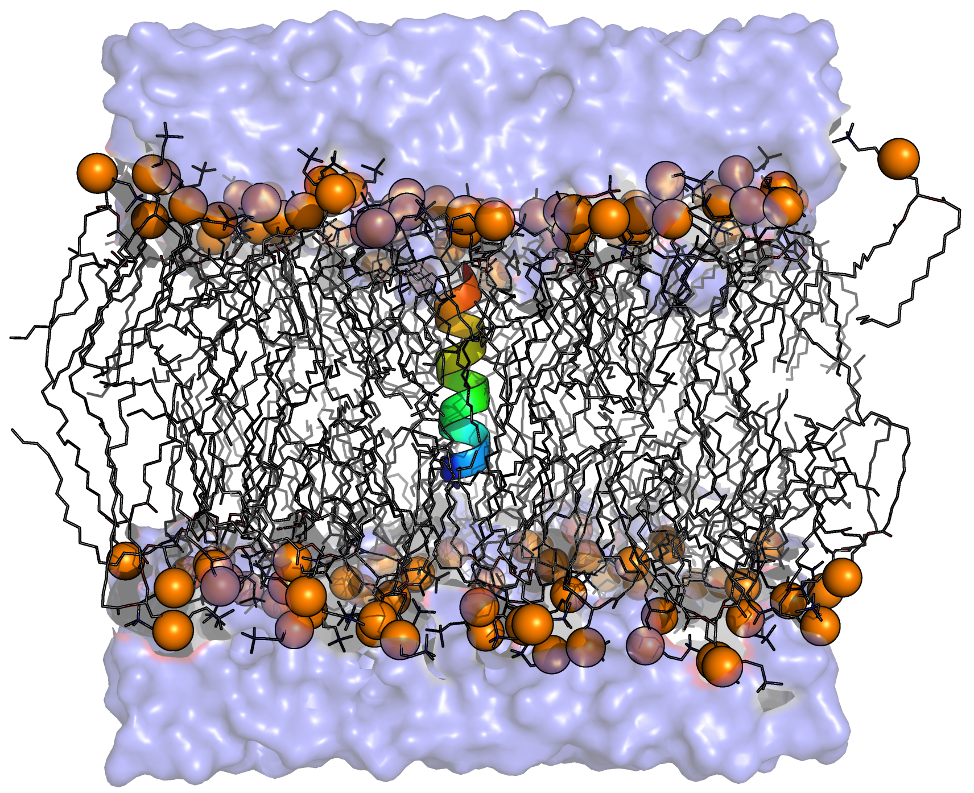
\includegraphics{kalp15_dppc}
\caption{The KALP\textsubscript{15} model peptide, embedded in a hydrated DPPC bilayer.}
\label{kalp_dppc_fig}
\end{figure}

Membrane proteins are of substantial biological interest as they modulate signaling pathways, engage in cell-cell interactions, and frequently serve as drug targets. Given their hydrophobicity, membrane proteins are difficult to crystallize or otherwise study experimentally. Thus, MD simulations serve as a useful technique in describing membrane protein conformational ensembles and protein-lipid interactions. Preparing a membrane protein system (Figure!\ref{kalp_dppc_fig}) is somewhat more difficult than a simple protein in water, as there are additional steps required to embed the protein in a membrane and carefully equilibrate these heterogeneous systems. This tutorial is available at \tutorialkalp.

\subsubsection{Prepare the Protein Topology} \label{kalp_protein_topology}

Model peptides are useful for studying protein-lipid interactions. The peptide that is the subject of this tutorial is called "KALP\textsubscript{15}" and has a sequence of Ac-GKK(LA)\textsubscript{4}LKKA-NH\textsubscript{2}. The "Ac" and "NH\textsubscript{2}" correspond to acetyl and amide groups, respectively. This peptide was the subject of an investigation on hydrophobic mismatch performed by Kandasamy and Larson~\cite{Kandasamy2006}. That study motivated the present tutorial.

The input coordinate file for the KALP\textsubscript{15} peptide can be constructed with programs that can build arbitrary molecules. In this tutorial, the peptide was initially built in the xLeap program of AmberTools (\url{http://ambermd.org/}) but could also be built with CHARMM~\cite{Brooks2009} if the user prefers. The initial geometry was set to that of an ideal $\alpha$-helix ($\phi$ = -60\textdegree, $\psi$ = -45\textdegree). This coordinate file was aligned along the {\em z}-axis (which, as will be shown later, corresponds to the membrane normal) by using the GROMACS \texttt{editconf} program, which has an option called \texttt{-princ} that aligns the longest axis of the provided coordinates along the {\em x}-axis. A subsequent rotation of 90\textdegree about the {\em y}-axis (also with \texttt{editconf}) aligns the peptide with the {\em z}-axis. A properly aligned KALP\textsubscript{15} peptide coordinate file is provided in the online tutorial.

The topology for this system will be generated with the GROMOS96 53A6 force field~\cite{Oostenbrink2004}. When executing \texttt{pdb2gmx}, the user should choose "None" for both the N- and C-termini. As described above, the N- and C-termini are capped with acetyl and amide groups, respectively. Without these groups, the peptide would have a large dipole moment as a result of the free amine (-NH\textsubscript{3}\textsuperscript{+}) and carboxylate (-COO\textsuperscript{$-$}) groups that would give rise to artificial dynamics. Model peptides are often capped to avoid these spurious "end effects."

Invoke \texttt{pdb2gmx} to produce the topology:

\begin{lstlisting}
$ gmx pdb2gmx -f KALP-15_princ.pdb -o KALP-15_processed.gro -ignh -ter -water spc
\end{lstlisting}

Note the use of the \texttt{-ignh} option above. The initial coordinates are an all-atom model. GROMOS96 is a united-atom force field, meaning that nonpolar hydrogen atoms are merged into their parent carbon atoms. This convention means there are fewer atoms in the system and thus the simulation will proceed more quickly. Using \texttt{-ignh} allows \texttt{pdb2gmx} to ignore all hydrogen atoms and rebuild only those required by the force field.

It is important to note here that united-atom force fields are not very commonly used. In the past, when computing power was much lower, it was desirable to limit the number of atoms in the system. All modern force fields had their origins in united-atom parameter sets~\cite{Gelin1979,Weiner1984,Jorgensen1984}. In the present tutorial, a united-atom force field will be used as it is convenient for demonstrating the principles necessary to construct the membrane protein system and manipulate the underlying force field files. With phospholipids, the reduction in the number of atoms in the system is also quite dramatic, leading to considerable increase in simulation speed.

\subsubsection{Customize the Force Field} \label{kalp_ff}

The topology generated in Section~\ref{kalp_protein_topology} describes only the protein, and the GROMOS96 53A6 parameter set (as distributed with GROMACS) does not contain topologies or parameters for phospholipids. Recently, such parameters have been published~\cite{Kukol2009}. In this tutorial, we will apply an older, but widely used, united-atom lipid force field derived by Berger, Edholm, and J{\"a}hnig~\cite{Berger1997}.

\begin{figure}[h!]
\centering
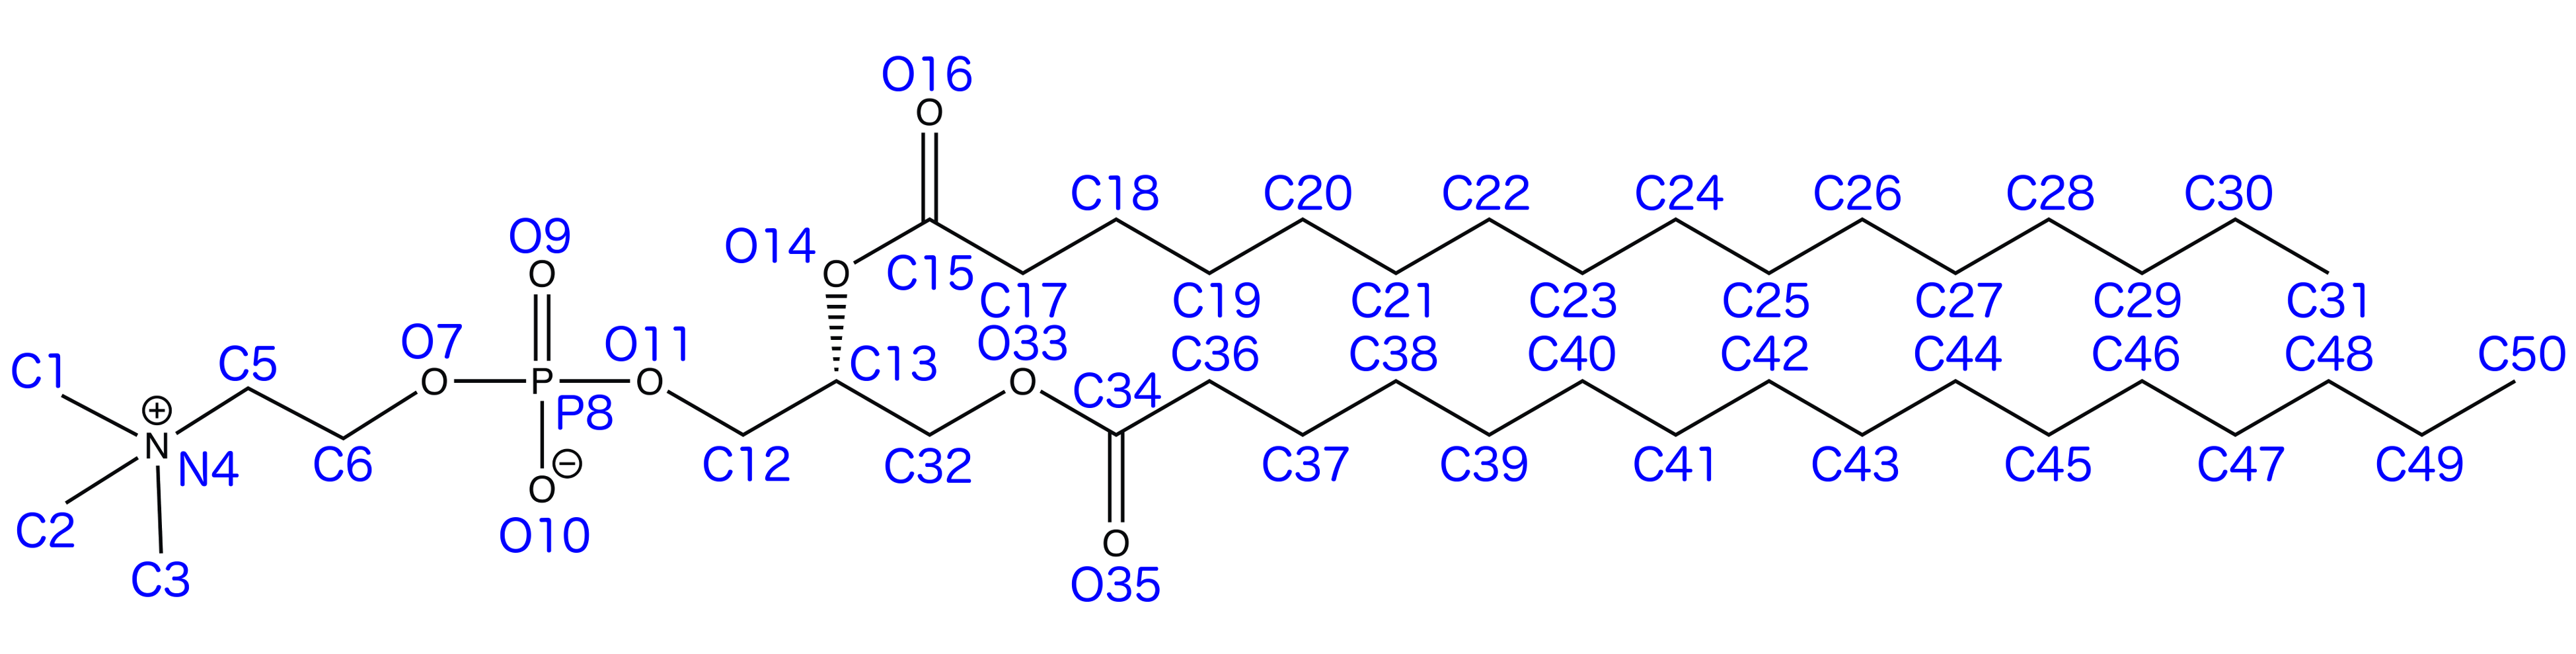
\includegraphics{DPPC_new_label}
\caption{The chemical structure of the DPPC lipid, with atom names according to the Berger lipid force field. The {\em sn-1} chain begins at carbon C34 and the {\em sn-2} chain begins at carbon C15.}
\label{kalp_dppc_structure_fig}
\end{figure}

The phospholipid used in this tutorial is dipalmitoylphosphatidylcholine (DPPC, Figure~\ref{kalp_dppc_structure_fig}). It is a fully saturated, zwitterionic membrane lipid that is often used in simple models of membranes. The topology and force field parameters for DPPC using the Berger parameters are distributed by Prof. D. Peter Tieleman at the University of Calgary. Download the following files from his website (\url{http://wcm.ucalgary.ca/tieleman/downloads}):

\begin{enumerate}
	\item{\texttt{dppc128.pdb}: Coordinates of a 128-lipid DPPC bilayer}
	\item{\texttt{dppc.itp}: The topology of DPPC, containing its\\ \texttt{[moleculetype]} definition}
	\item{\texttt{lipid.itp}: The Berger lipid force field parameters}
\end{enumerate}

The \texttt{lipid.itp} file is a self-contained, full force field for the Berger phospholipids. It is distributed in a standalone form, such that it can be used directly for simulating pure lipid membranes. To utilize it in the context of a membrane protein system, it must be incorporated into the existing force field that describes the protein. Rather than using it directly, the user must add the parameters from \texttt{lipid.itp} into the appropriate GROMOS96 53A6 force field files. To do so, make a local copy of the force field directory into the working directory (assuming GROMACS is installed in the standard location of \texttt{/usr/local/gromacs}):

\begin{lstlisting}[basicstyle=\footnotesize\ttfamily]
$ cp -r /usr/local/gromacs/share/gromacs/top/gromos53a6.ff/ ./gromos53a6_lipid.ff
\end{lstlisting}

A full explanation of the force field files in this new directory is given in the online version of the tutorial. The files that will be modified as part of this tutorial are:

\begin{enumerate}
	\item{\texttt{ffbonded.itp}: The bonded force field parameters (bonds, angles, dihedrals, and improper dihedrals)}
	\item{\texttt{ffnonbonded.itp}: The nonbonded force field parameters (atom types, Lennard-Jones parameters, pair interactions)}
\end{enumerate}

The modifications to the force field files must be made carefully to have a functional force field. First, copy the contents of the \texttt{[atomtypes]}, \texttt{[nonbond\_params]}, and \texttt{[pairtypes]} directives in \texttt{lipid.itp} into the corresponding sections of \texttt{ffnonbonded.itp}. The \texttt{[atomtypes]} section of \texttt{lipid.itp} lack atomic numbers and must be added in. In the \texttt{[nonbond\_params]} section (which defines pair-specific Lennard-Jones interactions, {\em e.g.} those that do not obey normal combination rules), delete the line that says \texttt{;; parameters for lipid-GROMOS interactions}. Delete this line and all the lines that follow in the \texttt{[nonbond\_params]} section. These entries correspond to GROMOS87 atom types and interactions that are not necessary or appropriate when using the GROMOS96 53A6 force field. Similarly, delete or comment out (with ;) any line in \texttt{[nonbond\_params]} that includes "HW," which is also not a valid atom type in GROMOS96. It indicates water hydrogen atoms, but these are simply called "H" in GROMOS96. Thus, one can also simply replace "HW" with "H" to avoid future errors. Failure to do these steps properly will lead to fatal errors when using \texttt{grompp}.

After modifying \texttt{ffnonbonded.itp}, add the contents of the \texttt{lipid.itp} \texttt{[dihedraltypes]} section to the equivalent section in \texttt{ffbonded.itp}.

These modifications of the force field files are fairly significant, and it is important to carefully check to make sure all steps have been completed correctly.

\begin{Checklists}
\begin{checklist}{Force Field Modifications}
\begin{itemize}
	\item{Copy the contents of \texttt{[atomtypes]} from \texttt{lipid.itp} to \texttt{ffnonbonded.itp} and add atomic numbers to each}
	\item{Copy the contents of \texttt{[nonbond\_params]} from \texttt{lipid.itp} to \texttt{ffnonbonded.itp}}
	\item{Remove the \texttt{;; parameters for lipid-GROMOS \\interactions} line and all subsequent lines in \\\texttt{[nonbond\_params]} from \texttt{ffnonbonded.itp}}
	\item{Remove or comment out any line in \texttt{[nonbond\_params]} in \texttt{lipid.itp} containing "HW," or rename to "H"}
	\item{Copy the contents of \texttt{[pairtypes]} from \texttt{lipid.itp} to \texttt{ffnonbonded.itp}}
	\item{Copy the contents of \texttt{[dihedraltypes]} from \texttt{lipid.itp} to \texttt{ffbonded.itp}}
\end{itemize}
\end{checklist}
\end{Checklists}

Next, to make use of the modified force field, an adjustment to the system topology (\texttt{topol.top}) must be made. Change the call to the force field from:

\begin{lstlisting}[basicstyle=\small\ttfamily]
#include "gromos53a6.ff/forcefield.itp"
\end{lstlisting}
%
to:

\begin{lstlisting}[basicstyle=\small\ttfamily]
#include "gromos53a6_lipid.ff/forcefield.itp"
\end{lstlisting}

Finally, add an \texttt{\#include} statement to add the DPPC topology to the system topology, in the exact location shown (to avoid disrupting any other \texttt{[moleculetype]} in the topology:

% \begin{lstlisting}[basicstyle=\footnotesize\ttfamily]
\begin{lstlisting}[basicstyle=\small\ttfamily]
; Include Position restraint file
#ifdef POSRES
#include "posre.itp"
#endif

; Include DPPC chain topology
#include "dppc.itp"

; Include water topology
#include "gromos53a6_lipid.ff/spc.itp"
\end{lstlisting}

At this point, some additional discussion on force field choice is warranted. The use of GROMOS96 53A6 to treat the protein and the Berger united-atom lipid parameters for DPPC is motivated by several factors. First, the constructed system (KALP\textsubscript{15} in DPPC) is a reproduction of a published and well-studied system~\cite{Kandasamy2006}. Second, the Berger lipid parameters are compatible with the GROMOS protein parameter set. Finally, the modification of the force field files is a useful instructive tool in teaching new users how this information is organized in GROMACS, allowing for future modifications in advanced systems. However, any MD simulation must be carefully planned, which includes a critical assessment of force field parameters for all species in the system. One should not automatically choose this force field combination simply because this tutorial does. In fact, the GROMOS96 53A6 force field has been shown to under-stabilize $\alpha$-helices~\cite{Schmid2011}, and the Berger parameters are not necessarily the best representation of lipid properties, particularly for DPPC. A useful reference is a systematic study by Piggot et al.~\cite{Piggot2012}, though the lipid force field literature is rich with other comparisons. Users must carefully consider available studies that critically assess force field performance for any system, but phospholipid membranes are especially challenging, and while no force field perfectly represents all relevant parameters, some force fields are demonstrably better than others.

\subsubsection{Construct the System} \label{kalp_construct}

\begin{figure*}[h!]
\centering
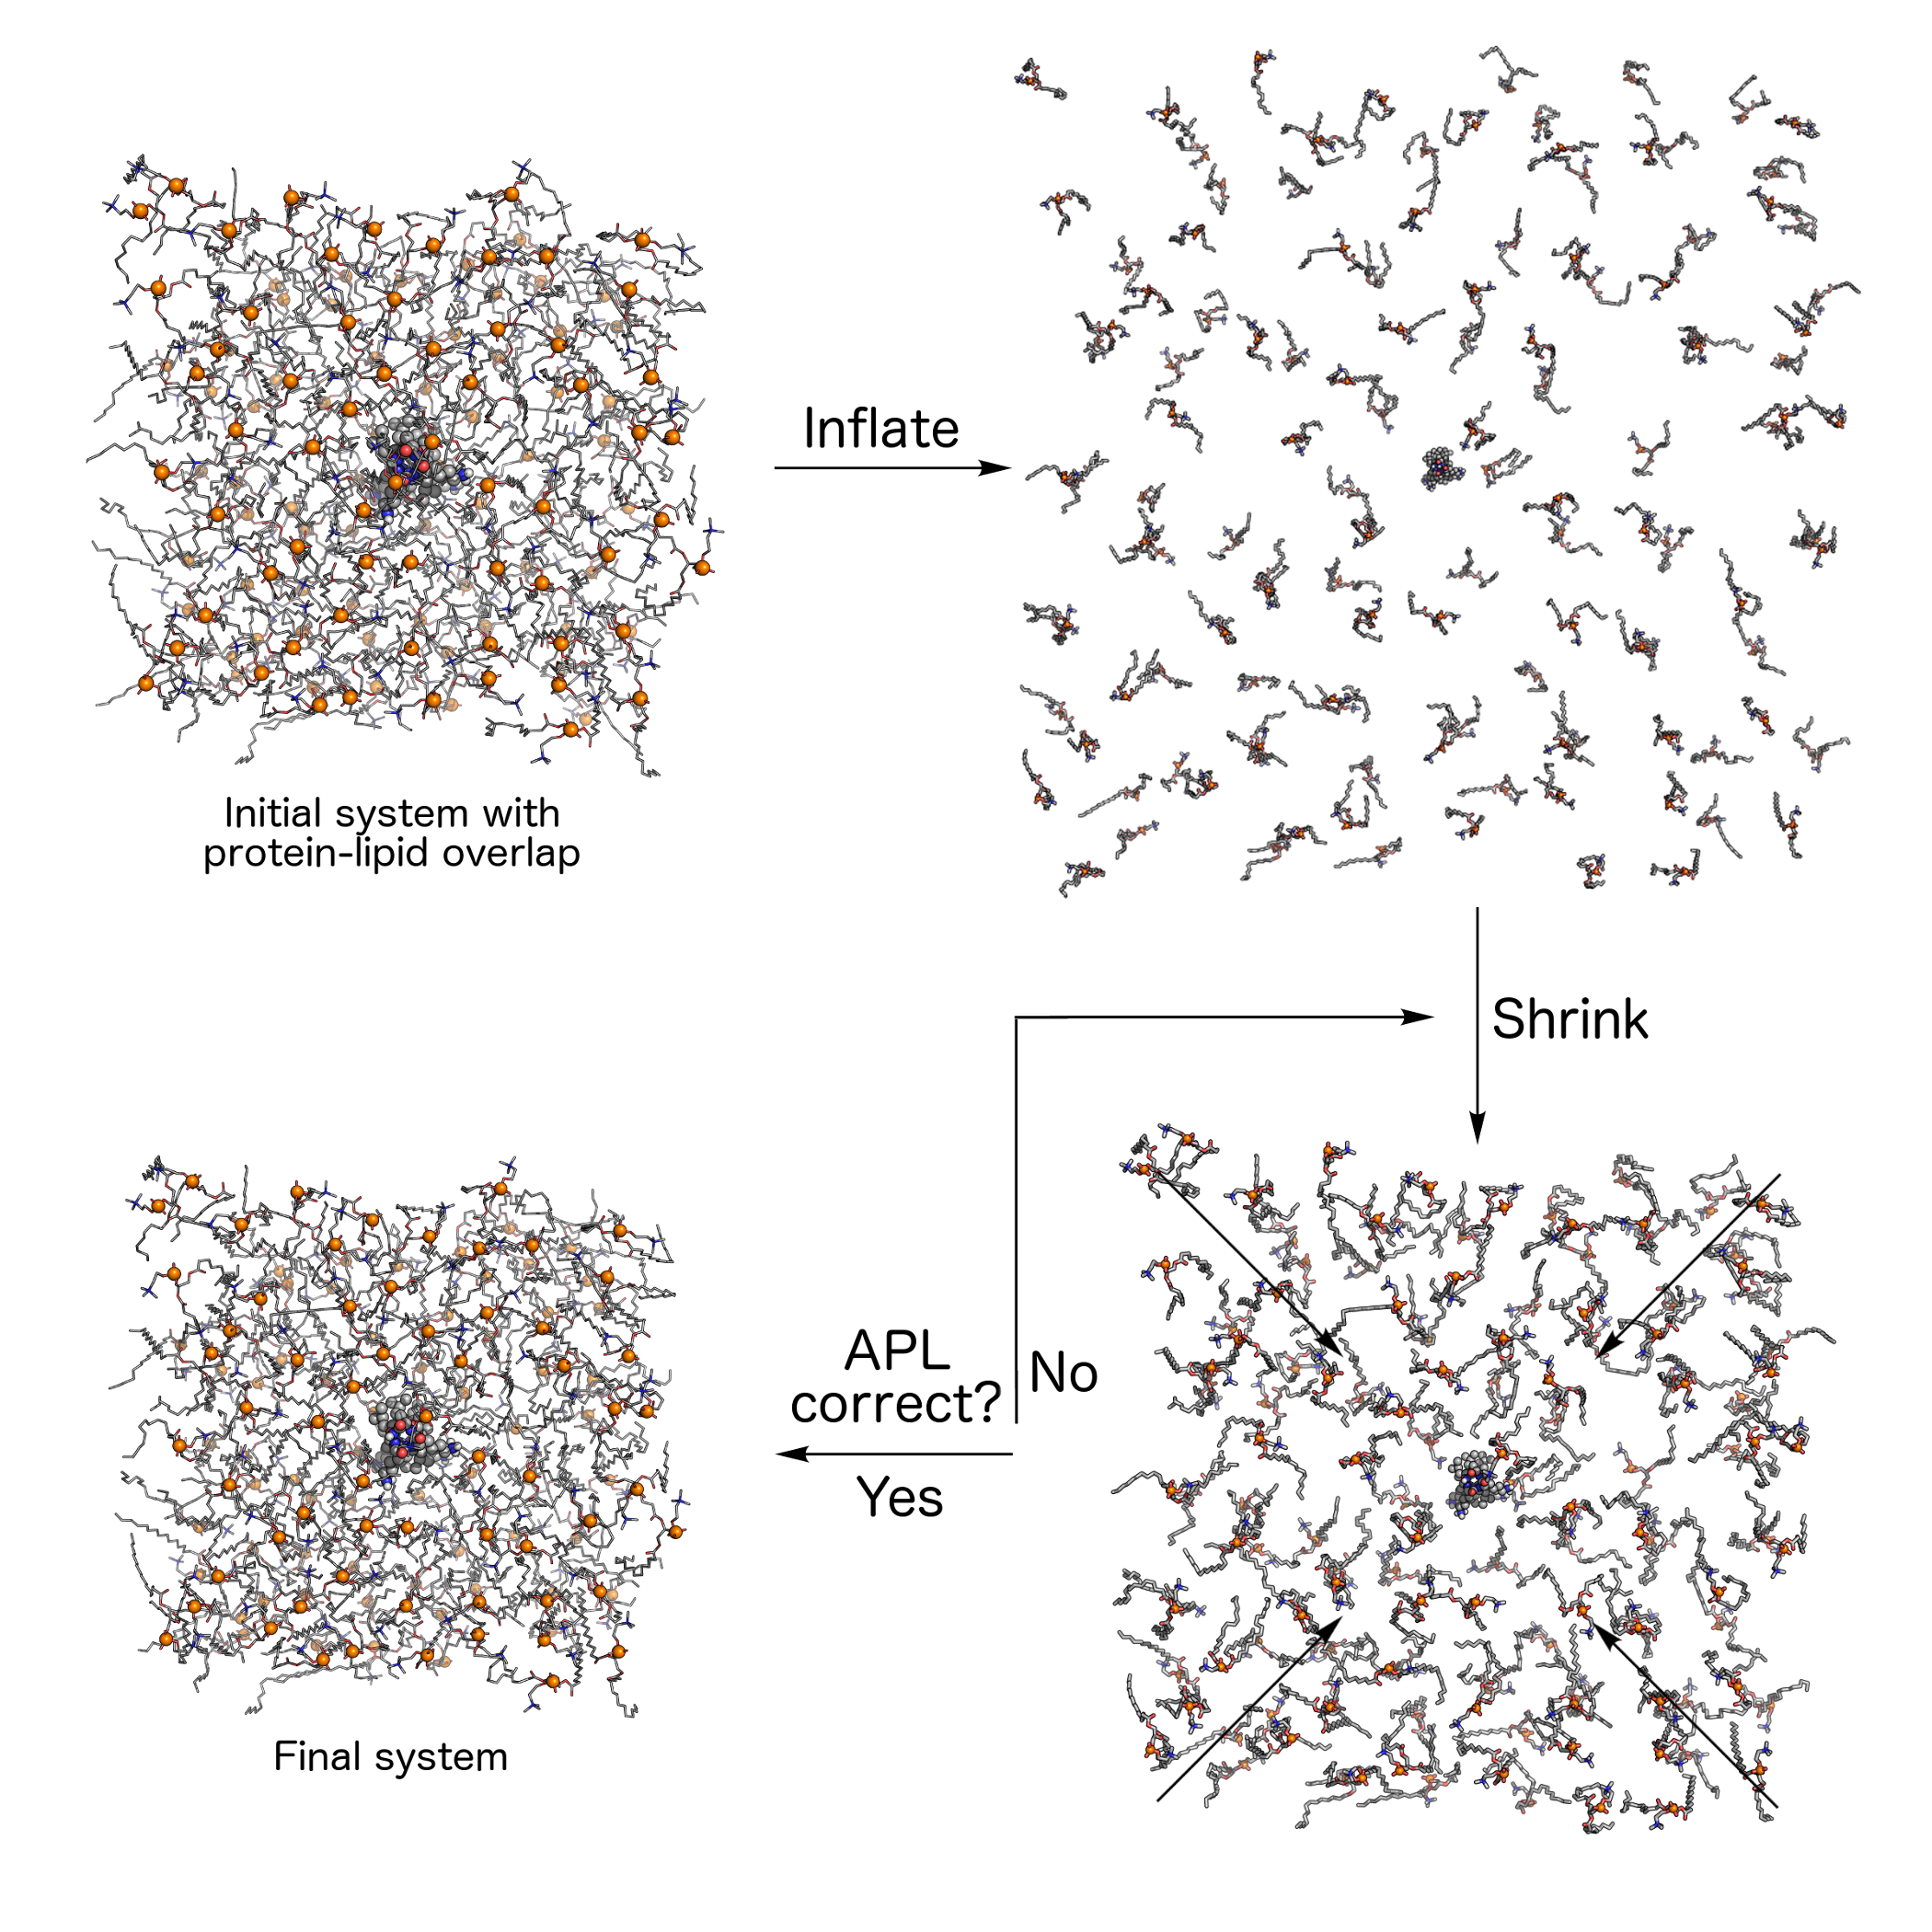
\includegraphics{kalp_dppc_lipid_pack}
\caption{The process of packing DPPC lipids around the KALP\textsubscript{15} peptide. The initial lipid coordinates, with protein-lipid atomic overlap, are scaled outward by some inflation factor (4 in this tutorial) and any lipids that remain overlapping with the protein are deleted. The scaling vector is reduced to a value < 1 to shrink the system (inward movement denoted by arrows pointing in from corners). The shrinking process is carried out iteratively until a reasonable APL value is achieved, yielding the final, packed system that is prepared for solvation with water.}
\label{kalp_lipid_pack}
\end{figure*}

The force field and system topology files are now fully prepared to describe the contents of the membrane-protein system being constructed. As in Tutorial 1 (Section~\ref{lyso}), the next step after preparing the initial topology is solvation. In nearly all MD simulations of biomolecules, the solute of interest is embedded within some type of liquid solvent, which in this case will be comprised of both a phospholipid bilayer and water. In contrast to the simple addition of a homogeneous solvent using \texttt{solvate}, the addition of the lipids around the protein requires auxiliary methods. In this tutorial, the DPPC lipids will be packed around the KALP\textsubscript{15} peptide using the InflateGRO method~\cite{Kandt2007}. With this approach, the lipid coordinates are scaled in the {\em x-y} plane, any lipids that remain overlapping with the protein are deleted, and then the lipids are progressively packed around the protein with intervening rounds of energy minimization.

The DPPC coordinate file distributed by Prof. Tieleman has "broken" lipids; all atoms are "inside" the central image and have the appearance that the lipid molecules are not bonded across periodic boundaries. While this representation is perfectly valid for carrying out MD simulations, InflateGRO will not work unless the molecules are "intact," that is, the distance between bonded atoms is at a minimum with respect to the periodic unit cell. To produce a correct coordinate file for InflateGRO, build a \texttt{.tpr} file that corresponds to the DPPC-water system. A topology for this system (\texttt{topol\_dppc.top}) is provided as part of the online tutorial. Any syntactically valid \texttt{.mdp} file can be used for this purpose. Note that \texttt{topol\_dppc.top} is only used in this step and never again. Any updates or reference to the system topology described in the tutorial are in \texttt{topol.top}.

Create the \texttt{.tpr} file:

\begin{lstlisting}
$ gmx grompp -f minim.mdp -c dppc128.pdb -p topol_dppc.top -o dppc.tpr
\end{lstlisting}

Invoke \texttt{trjconv}:

\begin{lstlisting}
$ gmx trjconv -s dppc.tpr -f dppc128.pdb -o dppc128_whole.gro -pbc mol -ur compact
\end{lstlisting}

Next, the KALP\textsubscript{15} peptide must be centered within the same box as the DPPC bilayer, such that the membrane center and peptide center are coincident. Open \texttt{dppc128\_whole.gro} in a text editor and navigate to the last line of the file (or, on the command line, use \texttt{tail -n 1 dppc128\_whole.gro}). The last line of a \texttt{.gro} file contains the box vectors of the system. Center the KALP\textsubscript{15} peptide in a box with the same dimensions as that of the DPPC bilayer with \texttt{editconf}:

\begin{lstlisting}
$ gmx editconf -f KALP-15_processed.gro -o KALP_newbox.gro -c -box 6.41840 6.44350 6.59650
\end{lstlisting}

The next step in assembling the system is to prepare the input coordinates for use in InflateGRO. To do so, concatenate the protein and membrane coordinates:

\begin{lstlisting}
$ cat KALP_newbox.gro dppc128_whole.gro > system.gro
\end{lstlisting}

The \texttt{system.gro} file is not formatted correctly. A valid \texttt{.gro} file has the following format:

\begin{lstlisting}
Title
  Number of atoms
  (all lines containing atomic coordinates)
Box vectors
\end{lstlisting}

By concatenating two \texttt{.gro} files together, there are now unnecessary lines that need to be removed. Open \texttt{system.gro} in a text editor and search down for "DPPC." Above the first occurrence of lipid coordinates are three lines that need to be removed: (1) the box vectors from \texttt{KALP\_newbox.gro}, (2) the title line from \texttt{dppc128\_whole.gro}, and (3) the number of atoms from \texttt{dppc128\_whole.gro}. Prior to removing the line containing the number of atoms, make note of it. After removing it, add this number to the second line in the file, to specify the total number of atoms in the system. Save the file and exit the text editor. Note that one can easily validate the number of atoms in the file with the Linux \texttt{wc} command:

\begin{lstlisting}
$ wc -l system.gro
\end{lstlisting}

Subtract three from the number reported by \texttt{wc} (to reflect the title line, number of atoms line, and box vectors). This number should match what appears on the second line of the \texttt{.gro} file. If it does not, inspect the file to determine the source of discrepancy, and if it does not match, start over with the \texttt{cat} command above. A quick test for validity of \texttt{system.gro} is to open it in some visualization software like VMD. If the file does not open or the program reports an error, it has been constructed incorrectly.

The InflateGRO method requires strong position restraints to be placed on the protein being embedded in the lipid membrane, beyond the default value of 1000 kJ mol\textsuperscript{-1} nm\textsuperscript{-2} written in \texttt{posre.itp} from \texttt{pdb2gmx}~\cite{Kandt2007}. To create a new file, with stronger restraints (100000 kJ mol\textsuperscript{-1} nm\textsuperscript{-2}), invoke the \texttt{genrestr} program, choosing "Protein" when prompted:

\begin{lstlisting}
$ gmx genrestr -f KALP_newbox.gro -o strong_posre.itp -fc 100000 100000 100000
\end{lstlisting}

Add an \texttt{\#ifdef} statement to call the new \texttt{strong\_posre.itp} file in \texttt{topol.top}:

\begin{lstlisting}
; Include Position restraint file
#ifdef POSRES
#include "posre.itp"
#endif

; Strong position restraints for InflateGRO
#ifdef STRONG_POSRES
#include "strong_posre.itp"
#endif

; Include DPPC chain topology
#include "dppc.itp"

; Include water topology
#include "gromos53a6_lipid.ff/spc.itp"
\end{lstlisting}

The coordinates and topology are now ready to be processed with the InflateGRO Perl script:

\begin{lstlisting}
$ perl inflategro.pl system.gro 4 DPPC 14 system_inflated.gro 5 area.dat
\end{lstlisting}

The order of command-line arguments passed to InflateGRO is specific and must adhere to this exact order. The syntax is as follows:

\begin{enumerate}
	\item{\texttt{system.gro}: the input coordinate file to which scaling is applied}
	\item{\texttt{4}: the scaling factor applied. A value > 1 indicates inflation (expansion) and a value < 1 indicates shrinking (compression)}
	\item{\texttt{DPPC}: the residue name of the lipids to which scaling is applied}
	\item{\texttt{14}: the cutoff radius (in \AA) for searching for lipids to delete}
	\item{\texttt{system\_inflated.gro}: the output coordinate file name}
	\item{\texttt{5}: the grid spacing for calculation of area per lipid}
	\item{\texttt{area.dat}: the name of the text file to which area per lipid values are printed}
\end{enumerate}

InflateGRO will print to the screen how many lipids are deleted. Note this value and update the \texttt{[molecules]} section of \texttt{topol.top} accordingly. It is also important to note that InflateGRO removes all water molecules. The user must not add back any water molecules until the lipids are completely packed around the protein. Therefore, \texttt{[molecules]} should refer only to the protein and the DPPC lipids. Do not invoke \texttt{solvate} until instructed to later in this tutorial.

The system now requires energy minimization. The\\ \texttt{minim\_inflategro.mdp} file (provided online) includes a line that reads:

\begin{lstlisting}
define = -DSTRONG_POSRES
\end{lstlisting}

With this command, the strong position restraints will be applied to the protein heavy atoms during all energy minimizations carried out while packing the lipids around the protein with InflateGRO.

Perform energy minimization, being sure to use explicit file names. As there will be many rounds of packing and energy minimization, relying on default GROMACS file names is not recommended. Minimize the inflated system using descriptive file names:

\begin{lstlisting}
$ gmx grompp -f minim_inflategro.mdp -c system_inflated.gro -p topol.top -r system_inflated.gro -o system_inflated_em.tpr

$ gmx mdrun -deffnm system_inflated_em
\end{lstlisting}

\begin{figure*}[h!]
\centering
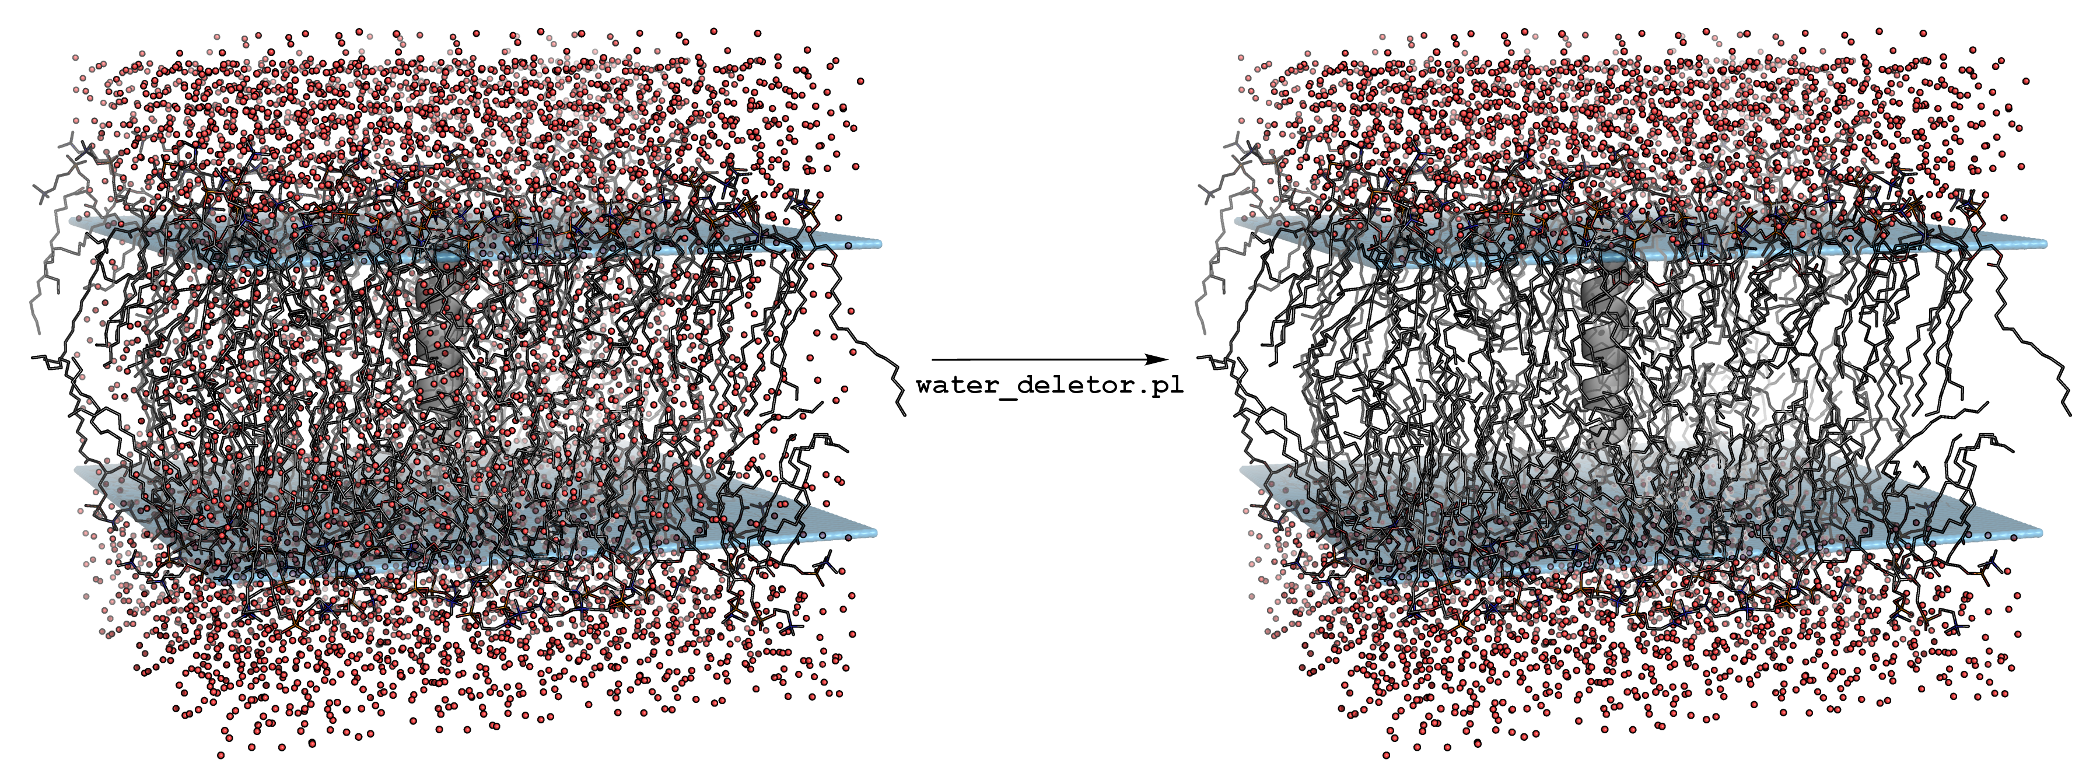
\includegraphics{kalp_dppc_water_deletor}
\caption{The action of the \texttt{water\_deletor.pl} script. Water molecules with {\em z}-coordinates that fall between the O33 atoms (which define the translucent blue planes) are deleted, leaving a hydrated bilayer with no water molecules within the hydrophobic core.}
\label{kalp_lipid_water_delete}
\end{figure*}

As before, the user must reconstruct the "broken" lipids before attempting to use the coordinate file further:

\begin{lstlisting}
$ gmx trjconv -s system_inflated_em.tpr -f system_inflated_em.gro -o tmp.gro -pbc mol

$ mv tmp.gro system_inflated_em.gro
\end{lstlisting}

The use of \texttt{tmp.gro} is necessary as \texttt{trjconv} returns an error when trying to read from, and write to, the same file name when correcting for PBC effects.

After the first energy minimization, the lipids need to be packed around the protein. To do so, use InflateGRO to apply a scaling factor that is less than 1. Doing so moves the lipids towards the protein. It is wise to do this packing very slowly to prevent intermolecular clashes that will lead to an unstable system. A typical scaling factor during packing is 0.95. To perform the first shrinking/packing step, invoke InflateGRO as follows:

\begin{lstlisting}
$ perl inflategro.pl system_inflated_em.gro 0.95 DPPC 0 system_shrink1.gro 5 area_shrink1.dat
\end{lstlisting}

Note that the cutoff radius has also been reduced to 0 \AA. Such a cutoff value disables the deletion of lipids. It is only appropriate to delete lipids during inflation; if the cutoff value is retained, eventually all of the lipids (or a great many of them) will be deleted and the system will be useless. After 26 rounds of packing (shrinking the lipids inward, energy minimization, and reconstruction of "broken" lipids), an area per lipid of roughly 71 \AA\textsuperscript{2} should be attained. Since InflateGRO overestimates area per lipid slightly, this value is an indication that additional shrinking is not necessary. That is, it is not necessary to achieve the exact experimental value of area per lipid (62 \AA\textsuperscript{2}). The online tutorial provides a Bash script that automates this process, but users wishing to learn via repetition can challenge themselves to carry out this process manually and become very comfortable with proper file naming. In summary, the process of packing lipids around the KALP\textsubscript{15} peptide is illustrated in Figure~\ref{kalp_lipid_pack}.

It is now time to add water to the system using \texttt{solvate}. One issue that will likely arise is that water molecules will be added within small void volumes in the hydrophobic core of the membrane. There are several strategies one can apply to deal with this situation, but the easiest is to allow \texttt{solvate} to add however many water molecules it can and subsequently delete those that fall within the membrane core. Solvate as usual with:

\begin{lstlisting}
$ gmx solvate -cp system_shrink26_em.gro -cs spc216.gro -p topol.top -o system_solv.gro
\end{lstlisting}

The online tutorial provides \texttt{water\_deletor.pl}, which is a simple Perl script that finds water molecules within a user-defined range of {\em z}-coordinate values and deletes them. The user defines a "reference" atom, which should be an atom in the ester region of the phospholipid and a "middle" atom defining the center of the membrane along its normal (typically the {\em z}-axis). See Figure~\ref{kalp_dppc_structure_fig} for atom naming in DPPC. From these atoms, the bilayer is divided into upper and lower leaflets, such that the reference atoms define the boundaries along the {\em z}-axis within which water molecules will be deleted (Figure~\ref{kalp_lipid_water_delete}). Finally, the script needs to know how many atoms constitute a water molecule. For SPC, there are 3 atoms (OW, HW1, and HW2), so this value is passed to the \texttt{-nwater} flag. Invoke the script as follows:

\begin{lstlisting}
$ perl water_deletor.pl -in system_solv.gro -out system_solv_fix.gro -ref O33 -middle C50 -nwater 3
\end{lstlisting}

\subsubsection{Add Ions} \label{kalp_ions}

Adding ions to the solvated KALP\textsubscript{15}-DPPC system is the same as any other system. Invoke \texttt{grompp} and \texttt{genion}:

\begin{lstlisting}
$ gmx grompp -f ions.mdp -c system_solv_fix.gro -p topol.top -o ions.tpr

$ gmx genion -s ions.tpr -o system_solv_ions.gro -p topol.top -pname NA -nname CL -neutral
\end{lstlisting}

Choose group 15 (SOL) for replacing water molecules with Cl\textsuperscript{$-$} ions.

\subsubsection{Energy Minimization} \label{kalp_em}

Energy minimization is performed in the same manner as any other system:

\begin{lstlisting}
$ gmx grompp -f minim.mdp -c system_solv_ions.gro -p topol.top -o em.tpr

$ mdrun -deffnm em
\end{lstlisting}

Energy minimization should converge rather quickly for this system, as the lipids were progressively relaxed around the protein prior to the addition of water:

\begin{lstlisting}[basicstyle=\footnotesize\ttfamily]
Steepest Descents converged to Fmax < 1000 in 292 steps
Potential Energy  = -3.2078762e+05
Maximum force     =  9.4299438e+02 on atom 130
Norm of force     =  5.1295775e+01
\end{lstlisting}

\subsubsection{Equilibration} \label{kalp_equil}

Equilibration of the KALP\textsubscript{15}-DPPC system will be carried out in two phases, as described in Section~\ref{lyso_equil}, an initial NVT equilibration followed by NPT equilibration. There are several important considerations specific to membrane simulations that are relevant at this stage. First, for the purposes of thermostatting and COM motion removal, the user will need to merge the atoms of the protein and DPPC groups using \texttt{make\_ndx}, a program that generates custom groups of atoms:

\begin{lstlisting}
$ gmx make_ndx -f em.gro -o index.ndx
\end{lstlisting}

Merge the protein (group 1) and DPPC (group 13) index groups with: \texttt{1 | 13}, type Enter, then type \texttt{q} and Enter to quit \texttt{make\_ndx}.

In equilibrating the lysozyme system (Section~\ref{lyso_equil}), temperature coupling groups were set to:

\begin{lstlisting}
tc-grps     = Protein Non-Protein
\end{lstlisting}

If the same syntax were used in the case of a membrane-protein system, the "Non-Protein" group would also contain the phospholipids. Doing so is undesirable due to the heterogeneity of the system. Lipids and water diffuse on different time scales, thus if they are treated in the same group for the purposes of thermostatting, there will be spurious contributions to the velocity scaling. As a consequence, it is common to treat the constituents of the membrane (all lipids and the embedded protein, whose diffusion depends strongly on the lipids) as a single group with respect to the thermostat. Merging the protein and DPPC lipids (above) allows the user to apply this convention. As such, the thermostat settings in \texttt{nvt.mdp} are:

\begin{lstlisting}
tcoupl      = V-rescale
tc-grps     = Protein_DPPC  Water_and_ions
tau_t       = 0.1           0.1
ref_t       = 323           323
\end{lstlisting}

The "Water\_and\_ions" group is a default group available in GROMACS, encompassing all SOL molecules and (in this case) Cl\textsuperscript{$-$} ions. Note, too, that the reference temperature is set to 323 K, above the experimental phase transition temperature of DPPC (315 K). For biological applications, it is generally desirable to perform membrane simulations above the phase transition temperature of the lipid membrane, such that it is in a liquid crystalline state. The reference temperature value should be determined not only in terms of the experimental value, but also in terms of the chosen force field. There may be some degree of error in how well a given force field models the phase transition of a given lipid, and the user must take this into account. A list of reference phase transition temperatures and associated literature references is provided in the online tutorial.

Similarly, the net COM motion removal in membrane systems (and any interfacial system, in general) must be given special consideration. Due to the differences in diffusion rates, one should set separate COM motion removal groups in the \texttt{.mdp} file. As such, in the \texttt{nvt.mdp} file, set:

\begin{lstlisting}
nstcomm     = 1
comm-mode   = Linear
comm-grps   = Protein_DPPC Water_and_ions
\end{lstlisting}

Perform NVT equilibration by calling \texttt{grompp} and \texttt{mdrun}:

\begin{lstlisting}
$ gmx grompp -f nvt.mdp -c em.gro -r em.gro -p topol.top -n index.ndx -o nvt.tpr

$ gmx mdrun -deffnm nvt
\end{lstlisting}

Following NVT, confirm that the temperature of the system stabilized at 323 K before continuing forward with NPT equilibration. It is also not uncommon to see some separation between the leaflets of the bilayer at the end of NVT. This void space will compress down and close during NPT equilibration.

In NPT equilibration, a new concept is introduced, semiisotropic pressure coupling. In this method, the coordinate scaling factors are uniform in the {\em x-y} plane but independent along the membrane normal, coincident with the {\em z}-axis. This approach reflects the intrinsic anisotropy in interfacial systems such as membranes, in which the lateral forces (among lipids) differ in magnitude from forces of water acting along the {\em z}-axis. The relevant pressure coupling settings in \texttt{npt.mdp} are:

\begin{lstlisting}
pcoupl          = Parrinello-Rahman
pcoupltype      = semiisotropic
tau_p           = 5.0
ref_p           = 1.0   1.0
compressibility = 4.5e-5    4.5e-5
\end{lstlisting}

The Parrinello-Rahman barostat was introduced previously, but is now employed in semiisotropic mode. There is only a single value of $\tau_p$, despite the ability to assign different reference pressures (\texttt{ref\_p} along {\em x-y} and {\em z}, respectively). The \texttt{compressibility} setting takes two values here, again along the membrane plane and normal, but the default value of the isothermal compressibility of water (4.5 $\times$ 10\textsuperscript{-5} bar\textsuperscript{-1}) is sufficient for this purpose. The compressibility affects the responsiveness of the barostat, not the physical properties of the medium. In principal, if one knows the lateral compressibility of the lipid, it could be substituted here, but given the dramatic range of instantaneous pressure values observed over the course of an MD simulation, it is unlikely that fine tuning this value will have any meaningful physical consequence and will not be done here.

Continue on with NPT equilibration:

\begin{lstlisting}
$ gmx grompp -f npt.mdp -c nvt.gro -r nvt.gro -p topol.top -t nvt.cpt -n index.ndx -o npt.tpr

$ gmx mdrun -deffnm npt
\end{lstlisting}

After equilibration, calculate the time-average pressure value and the time series of the {\em x}- and {\em y}- box vectors (Box-X and Box-Y, respectively, in the \texttt{energy} list of terms). The box vectors are an indication of the convergence of the lateral area of the system. While only a 1-ns simulation is unlikely to yield fully converged values (which can take from 50-100 ns to fully stabilize), a simple assessment here may be useful for obtaining an initial indication of the stability of the system.

\subsubsection{Production MD} \label{kalp_md}

Carry out a 1-ns production simulation, using the same NPT ensemble as during equilibration, but in the absence of position restraints on the protein:

\begin{lstlisting}
$ gmx grompp -f md.mdp -c npt.gro -t npt.cpt -p topol.top -n index.ndx -o md_0_1.tpr

$ gmx mdrun -deffnm md_0_1
\end{lstlisting}

It is important to note that 1 ns of time is orders of magnitude lower than what is normally required to obtain converged sampling in a membrane system. Typical simulations of these types of systems are in excess of 100 ns. The data obtained in this tutorial are for demonstration purposes only.

\subsubsection{Analysis} \label{kalp_ana}

There are many structural and dynamical properties of lipids that can be computed during an MD simulation. In the context of membrane-protein systems, many of these properties are interrelated with the dynamics of the protein, whether it is embedded (transmembrane) or peripherally associated. Lipid analysis requires great detail and often requires the use of custom index groups, which are user-generated selections of atoms on which the analysis is performed. In this section, several types of lipid-specific analysis will be introduced, along with proper construction of complex index groups.

\paragraph{Deuterium Order Parameters} \label{kalp_ana_scd}

The deuterium order parameter is a measure of the orientation of a C-D bond, thus reporting on the structure of hydrocarbons in layered systems. This quantity is defined as:

\begin{equation} \label{eq_scd}
-S_{CD} = \frac{\left\langle 3 cos^2 \theta - 1\right\rangle}{2}
\end{equation}
%
in which $\theta$ is the angle between the C-D bond and the membrane normal (again, the {\em z}-axis) and the angle brackets denote a time average. The GROMACS program that computes $-S_{CD}$ is called \texttt{order}. It requires an index file containing groups with all equivalent carbon atoms of the acyl chain in separate groups. To create such groups, refer to Figure~\ref{kalp_dppc_structure_fig}, in which the {\em sn-1} chain (referring to the "stereospecific number," {\em e.g.} the numbering in the glyercol backbone) includes carbon atoms C34 and C36-C50, inclusive, and the {\em sn-2} chain includes carbon atoms C15 and C17-C31, inclusive. To create these index groups, invoke \texttt{make\_ndx}:

\begin{lstlisting}
$ gmx make_ndx -f md_0_1.tpr -o sn1.ndx
> a C34
> a C36
> a C37
...
> a C50
> del 0-21
> q
\end{lstlisting}

The above commands passed to \texttt{make\_ndx} create individual groups with all C34, C36, C37, ... C50 atoms. The \texttt{del 0-21} command removes all the standard GROMACS groups, leaving only the lipid carbon atoms to be analyzed. The process should be repeated to create \texttt{sn2.ndx}, selecting the atoms indicated above.

To plot the deuterium order parameters for the {\em sn-1} chain, invoke \texttt{order}:

\begin{lstlisting}
$ gmx order -s md_0_1.tpr -f md_0_1.xtc -n sn1.ndx -d z -od deuter_sn1.xvg
\end{lstlisting}

It is important to note that the value of $-S_{CD}$ cannot be calculated for terminal carbon atoms, that is the carbonyl carbon (C34 in the {\em sn-1} chain) and the terminal methyl carbon (C50 in the {\em sn-1} chain). This limitation arises from the calculation of the local molecular axis. To compute this axis, the previous and next carbon atoms in the acyl chain are needed. For terminal carbon atoms, this axis is undefined. The output file (in this case, \texttt{deuter\_sn1.xvg}) from \texttt{order} is numbered from 1, as the program does not necessarily know which segment of the chain is being analyzed. For plotting purposes, edit the atom numbers in \texttt{deuter\_sn1.xvg} by incrementing each by 1. The resulting plot (after similarly analyzing the {\em sn-2} chain) will look something like what is shown in Figure~\ref{kalp_dppc_scd_fig}.

\begin{figure}[h!]
\centering
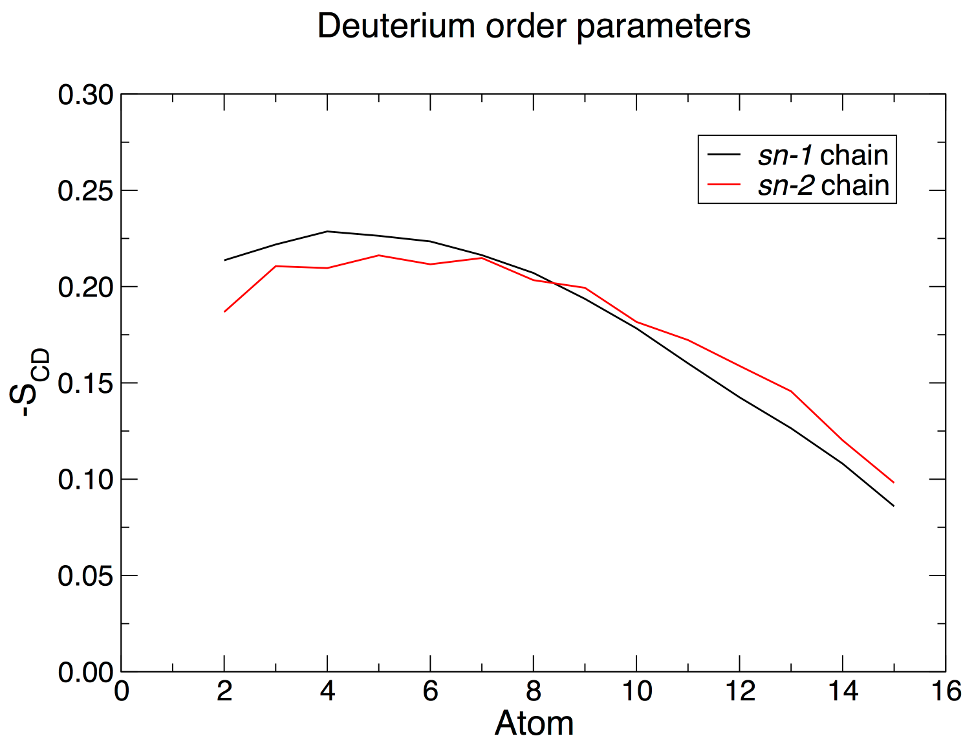
\includegraphics{plot_kalp_dppc_Scd}
\caption{Deuterium order parameters, $-S_{CD}$, of the palmitoyl chains in DPPC.}
\label{kalp_dppc_scd_fig}
\end{figure}

The resulting values of $-S_{CD}$ are indicative of DPPC lipids in a liquid crystalline form, as the plateau region (carbons 4-8) has a value of \textasciitilde0.2. This outcome is expected since (1) the starting DPPC coordinates were pre-equilibrated in a liquid crystalline state and the simulation carried out here is only for 1 ns, thus retaining this state and (2) the temperature during the simulation (323 K) was above the phase transition temperature of DPPC (315 K).

\paragraph{Membrane Density Profile} \label{kalp_ana_density}

The structure of phospholipid membranes can be described in part by computing a density profile along the membrane normal. The resulting plots show the relative positioning of the functional groups of the lipids. In this context, it is useful to subdivide the lipids into moieties with different properties or local structure, such as the headgroups (in this case, the zwitterionic phosphatidylcholine group), the glycerol or glycerol ester atoms, and the acyl chains. To create these groups, again refer to Figure~\ref{kalp_dppc_fig} for atom nomenclature and invoke \texttt{make\_ndx}:

\begin{lstlisting}
$ gmx make_ndx -f md_0_1.tpr -o density_groups.ndx
> 13 & a C1 | a C2 | a C3 | ... |  a O11
> name 22 Headgroups
> 13 & a C12 | a C13 | a O14 | a C15 |
  a O16 | a C32 | a O33 | a C34 | a O35
> name 23 Glycerol_Ester
> 13 & ! 22 & ! 23
> name 24 Acyl_Chains
> q
\end{lstlisting}

The selections created here are somewhat more complicated than any previously encountered in these tutorials. Group 13 is a default group containing all DPPC atoms. The use of ampersand (\&) denotes the intersection of selections, {\em i.e.} atoms belonging to both selections. The atoms are subsequently selected by their atom names ("a") and merged together using the pipe character (|) meaning "or." For the first group (Headgroups), the selection would literally read "atoms in DPPC that are also named either C1, C2, C3, ... or O11." The Glycerol\_Ester group is created similarly. The remaining atoms (those not in headgroups or the glycerol ester region) belong to the lipid acyl chains. Rather than typing out all of those atom names individually, the user can again employ logical operators. In creating the Acyl\_Chains group, use the logical "not" operator (!). The last selection translates to "atoms in DPPC that are not in the Headgroups group and also not in the Glycerol\_Ester group."

Use the \texttt{density} program to compute the partial densities of each of these groups:

\begin{lstlisting}
$ gmx density -s md_0_1.tpr -f md_0_1.xtc -n density_groups.ndx -o dens_headgroups.xvg -d Z
\end{lstlisting}

Select group number 22, then repeat the process for the glycerol ester, acyl chain, and water (SOL) groups. Plotting the files in XmGrace yields Figure~\ref{kalp_dppc_dens_fig}.

\begin{figure}[h!]
\centering
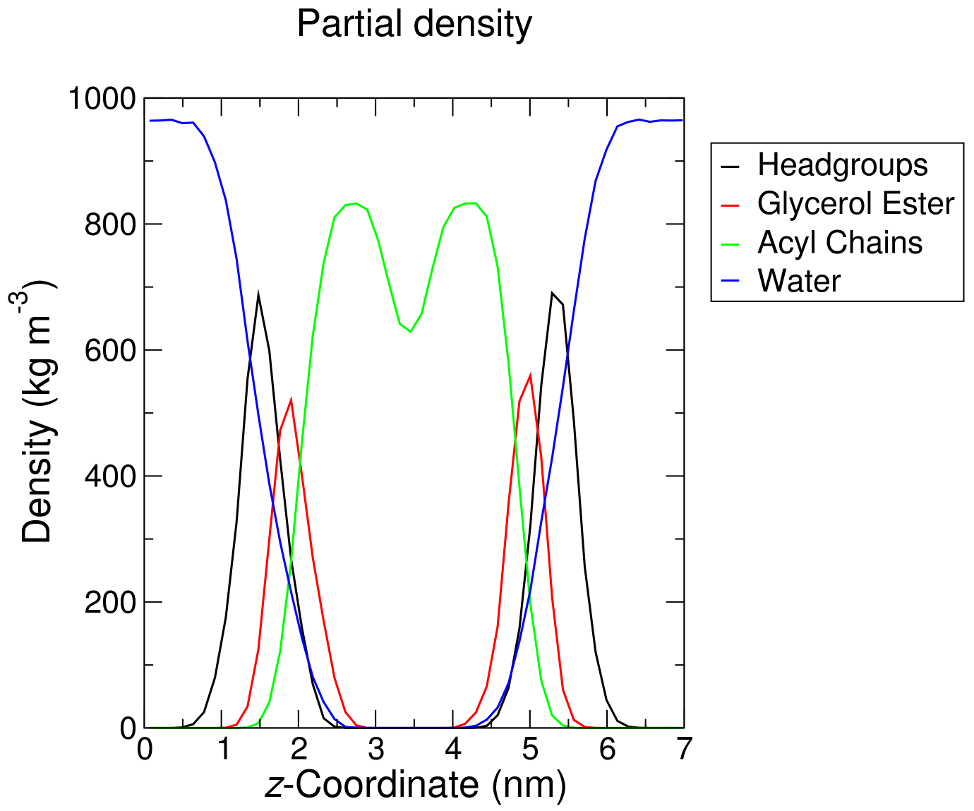
\includegraphics{plot_kalp_dppc_density}
\caption{Partial density profile of water and lipid functional groups along the {\em z}-axis.}
\label{kalp_dppc_dens_fig}
\end{figure}

\paragraph{Area Per Lipid and Bilayer Thickness} \label{kalp_ana_apl}

The lateral area per lipid (APL) is a way of assessing lipid packing, again reflecting gel or liquid-crystalline states. APL is related to the deuterium order parameters discussed above; large values of $-S_{CD}$ reflect acyl chain elongation, close packing, and thus smaller APL. Fluid membranes have larger APL than their gel-phase counterparts. GROMACS does not have a built-in program that computes APL. For a pure membrane (no protein), APL can be calculated simply from the {\em x}- and {\em y}- box vectors, {\em i.e.} APL = (Box-X $\times$ Box-Y) / (number of lipids per leaflet). When a protein is present, it occupies some amount of the lateral area in one or both leaflets. Several methods are available for computing APL in such a case. GridMAT-MD~\cite{Allen2009} is a program designed to interface directly with GROMACS, processing both \texttt{.gro} and \texttt{.pdb} coordinate files (including multi-frame files). It can also compute membrane thickness as a projection over the entire {\em x-y} plane, another feature that is absent in GROMACS.

\paragraph{Lateral Diffusion of Lipids} \label{kalp_ana_msd}

Calculating the lateral diffusion of lipids (that is, within the {\em x-y} plane) is often of interest in membrane systems, and as such, GROMACS provides a program, called \texttt{msd}, that computes the self-diffusion coefficient, $D_0$, of particles based on their mean-square displacement (MSD) using the Einstein relation~\cite{Allen1987}, {\em e.g.} for all particles $A$ running over index $i$: 

\begin{equation} \label{eq_msd}
\lim_{t\to\infty} \langle \norm{\mathbf{r}_i(t) - \mathbf{r}_i(0)}^2 \rangle_{i \in A} = 6D_{A}t
\end{equation}

The MSD can be computed by using a single atom within each molecule, or based on the COM of each molecule. Here, the MSD and resulting diffusion coefficient will be computed from a single, representative atom, the phosphorus (P8) in each DPPC lipid. First, construct an index group:

\begin{lstlisting}
$ gmx make_ndx -f md_0_1.tpr -o p8.ndx
...
> a P8
> q
\end{lstlisting}

Invoke \texttt{msd}:

\begin{lstlisting}
$ gmx msd -s md_0_1.tpr -f md_0_1.xtc -n p8.ndx -lateral z
\end{lstlisting}

The \texttt{-lateral} option instructs \texttt{msd} to calculate only the diffusion within the {\em x-y} plane, that is, the {\em z}-axis is normal to the plane of interest. The result from this simple system is likely to vary widely and is in no way converged or reflective of equilibrium lipid diffusion. From the limited number of data points, the statistical certainty of this value is likely to be poor, and a value like 2.7 $\pm$ 2.7 $\times$ 10\textsuperscript{-7} cm\textsuperscript{2} s\textsuperscript{-1} might be obtained. This value is neither accurate nor precise, and as such a much longer simulation would be required to obtain a more reliable value. For the purposes of this tutorial, this calculation serves as a cautionary note about the proper time scale required for performing simulations of lipid membranes. Interested users are encouraged to extend the simulation out to 50 or 100 ns and compare the values obtained over these time frames.

As a final note, it is important to recognize that periodic boundary conditions and the size of the box will influence the obtained value of $D_0$. In fact, the result obtained here is not truly $D_0$, it is a size-dependent quantity termed $D_{PBC}$ per Yeh and Hummer~\cite{Yeh2004}, who derived a correction factor that can be applied to obtain the true value of $D_0$ in periodic systems.

\subsubsection{Summary and Review of Objectives} \label{kalp_summary}

Through this tutorial, the user has been guided through the construction of a membrane-protein system, which requires modification of force field files and packing of lipids around the protein prior to solvation with water. To review, the objectives for this tutorial were as follows:

\begin{enumerate}
	\item Understand the organization and contents of GROMACS force field files and how parameters from different, but compatible, sources can be added to them
	\item Apply an iterative packing routine to place phospholipids around a transmembrane protein
	\item Perform lipid-specific analysis using custom index groups
\end{enumerate}

By adding parameters from an external force field file (in this case, \texttt{lipid.itp}) to an existing force field, the organization and logic of GROMACS force field files has been illustrated, with some discussion of the theory of force field compatibility. The solvation of a membrane-protein system has been approached through the use of an iterative packing scheme for the DPPC phospholipids, followed by conventional solvation with water and removal of water molecules within the hydrophobic core of the membrane with a custom script. These processes have required the user to become more familiar with GROMACS topology organization, including manual modification that was not required in the first tutorial. Finally, after performing a short simulation on the KALP\textsubscript{15}-DPPC system, several lipid-specific analyses were performed. Though the time scale of this simulation is insufficient to obtain converged data on lipid properties, the tutorial has provided the logic behind constructing complex index groups that are required for performing lipid analysis.



%%%%%%%%% TUTORIAL 3 %%%%%%%%%
\subsection{Tutorial 3: Umbrella Sampling} \label{pmf}

\begin{figure}[h]
\centering
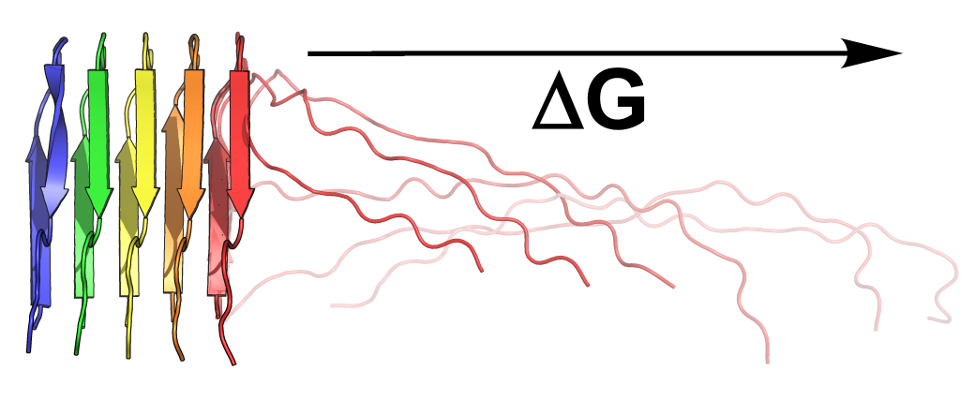
\includegraphics{umbrella_protofibril_dissociate}
\caption{The terminal peptide of the A$\beta$\textsubscript{42} protofibril dissociates along the fibril axis, the degree of freedom over which the free energy difference, $\Delta$G, is computed.}
\label{umbrella_composite_fig}
\end{figure}

It is often of interest to compute a free energy change that is associated with some change in geometry, such as a conformational change in a protein or the binding of two molecules as they approach each other along some path. Attempting to study such processes can be challenging with normal, unbiased MD simulations, as high-energy states (transition states or rare conformations) are not frequently sampled. Therefore, it is difficult to define accurate free energy differences, or the barriers may simply never be overcome on the timescale accessible to conventional MD. To overcome this challenge, biasing potentials can be applied to enhance sampling of these rare states and thereby more completely define free energy differences.

In this tutorial (available online at \tutorialpmf), the user will be guided through the process of calculating the free energy difference for the dissociation of a peptide from a pentameric assembly using umbrella sampling to compute the potential of mean force (PMF), or $\Delta$G (Figure~\ref{umbrella_composite_fig}). The process outlined here is based on a published study that examined the impact of point mutations on the stability of A$\beta$\textsubscript{42} protofibrils~\cite{Lemkul2010}. It is important to note here that these simulations are somewhat unique, as they involve extra restraints and only a single dimension along which the PMF is computed. Additional details will be provided in subsequent sections in the tutorial.

Constructing a system that will be subjected to umbrella sampling is much like any other, so the initial details of preparing the topology, defining the box, solvation, minimization, and equilibration will only highlight aspects that are unique to subsequent umbrella sampling simulations. Ultimately, to carry out these calculations, a set of configurations is generated along some path within the system (a distance, dihedral angle, etc.), called a "reaction coordinate," defining the starting points for each of a series of windows that allow sampling in discrete regions of the reaction coordinate. There are many ways to construct initial configurations in each window. In this tutorial, the reaction coordinate is defined as the $z$-axis and will employ a non-equilibrium technique called steered molecular dynamics (SMD) to generate the starting configurations for each window.

\subsubsection{Prepare the Protein Topology} \label{umbrella_protein_topology}

The system being studied here is a pentamer of the A$\beta$ peptide, in an aggregated fibril form. The initial coordinates are taken from an NMR structure determined by L\"uhrs et al.~\cite{Luhrs2005}. Each of the five protein chains is labeled (A, B, C, D, and E) in the PDB file, which is entry 2BEG. The first model (the lowest energy) will be used here, and the N-termini of each chain should be capped with acetyl groups to prevent spurious end effects. There are several residues in each chain that are disordered and therefore not assigned in the NMR structure. Residues 17-42 of each chain are present, so an acetyl cap should be added to Leu17 of each peptide. GROMACS has no ability to construct such terminal capping groups. As in the previous tutorial (Section~\ref{kalp_protein_topology}), these groups should be constructed in AmberTools (\url{http://ambermd.org/}) or CHARMM~\cite{Brooks2009}. A suitable protein PDB file is provided in the online version of the tutorial. With this file, execute \texttt{pdb2gmx}:

\begin{lstlisting}
$ gmx pdb2gmx -f 2BEG_model1_capped.pdb -o complex.gro -ignh -ter
\end{lstlisting}

Choose the GROMOS96 53A6 parameter set as the force field, and when prompted, choose "None" for all N-termini (to indicate the fact that no modifications should be made to acetyl groups) and "COO\textsuperscript{$-$}" for the C-termini (as Ala42 is the true C-terminus of the A$\beta$\textsubscript{42} peptide). The fact that there are multiple protein chains in the coordinates is not a problem for \texttt{pdb2gmx}, as it can produce a topology for each provided that the individual chains are either denoted with different chain identifiers (as is the case here) or delimited by TER cards.

Later, in Section~\ref{umbrella_smd}, a biasing force will be applied to one of the peptides (chain A) in the pentamer. To avoid distortions to the structure, restraints will be applied to chain B to immobilize it during this process. Note that \texttt{pdb2gmx} has produced individual topologies and restraint file topologies (all with extension \texttt{.itp}) for each chain. Add the following to the end of \texttt{topol\_Protein\_chain\_B.itp}:

\begin{lstlisting}
#ifdef POSRES_B
#include "posre_Protein_chain_B.itp"
#endif
\end{lstlisting}

It is important to note here that the input coordinates used in this tutorial differ from those used in our published study~\cite{Lemkul2010}. In that work, the pentamer was subjected to 100 ns of MD simulation to relax the initial configuration prior to being employed in PMF calculations. For simplicity in this tutorial, the input coordinates are taken directly from the NMR structure. Should the user wish to more faithfully replicate the published results, follow the protocol described in that work and use the final configuration of the system after 100 ns of MD as input into \texttt{pdb2gmx}.

\subsubsection{Define the Unit Cell and Solvate} \label{umbrella_box}

The box size for umbrella sampling simulations, like in any other system, must be set such that the minimum image convention (see Section~\ref{lyso_solv}) is satisfied at all times. There is an additional consideration, however, that requires the length of the biasing potential to also satisfy the minimum image convention. That is, the length of the biasing potential will be calculated from the minimum periodic distance between the restrained species that define the reaction coordinate. In this example, the reaction coordinate will be defined as the COM distance between chains A and B in the A$\beta$\textsubscript{42} protofibril, with a final length of 5.0 nm, sufficient to lead to complete dissociation of the two chains (no interactions within the longest nonbonded cutoff). The biasing potential will only be applied along the $z$-axis, therefore the length of the box along $z$ must be at least 10.0 nm (double the length of the reaction coordinate), with some additional space to satisfy the minimum image convention between the atoms in the system. The box vector along the $z$-axis will thus be set to 12.0 nm.

An orthorhombic box that defines a solute-box distance of 1.0 nm would result in a unit cell with dimensions of 6.560 nm $\times$ 4.362 nm $\times$ 4.955 nm, with the geometric center naturally following as (3.280, 2.181, 2.4775). To position the A$\beta$\textsubscript{42} protofibril in a manner sufficient to satisfy the minimum image convention with respect to the biasing potential in the newly defined box, use \texttt{editconf}:

\begin{lstlisting}
$ gmx editconf -f complex.gro -o newbox.gro -center 3.280 2.181 2.4775 -box 6.560 4.362 12
\end{lstlisting}

After doing so, the protofibril will be positioned within the unit cell as shown in Figure~\ref{umbrella_box_fig}.

\begin{figure}[H]
\centering
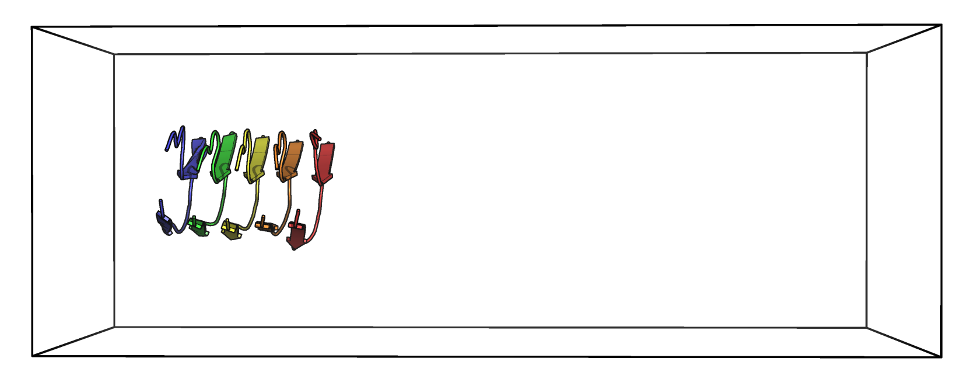
\includegraphics{umbrella_protofibril_box}
\caption{The position of the A$\beta$\textsubscript{42} protofibril in the unit cell.}
\label{umbrella_box_fig}
\end{figure}

It is important to note here that the approach taken thus far is fairly specific to the system being considered. The biasing potential will be applied directly along the $z$-axis, which is the fibril axis for A$\beta$ fibrils. The box size is designed to minimize the number of water molecules added, which is desirable since the box has to be large to accommodate the restraint length. It is possible to use a somewhat tight-fitting box in the $x-y$ plane since additional restraints will be applied to chain B of the protofibril. The restraints prevent the protofibril from rotating over time, therefore the box does not have to have spherical symmetry. In general, for {\em e.g.} protein-protein or protein-ligand binding, this approach would not work. The user would have to construct a cubic, rhombic dodecahedral, or truncated octahedral box and define a reaction coordinate in all three spatial dimensions. Because of the unique nature of the system being studied here, the approach is somewhat simplified in this tutorial. The biasing potential is as simple as possible and the system is relatively small so it will run quickly.

Proceed with solvation and the addition of 100 mM NaCl as in any other system:

\begin{lstlisting}
$ gmx solvate -cp newbox.gro -cs spc216.gro -o solv.gro -p topol.top

$ gmx grompp -f ions.mdp -c solv.gro -p topol.top -o ions.tpr

$ gmx genion -s ions.tpr -o solv_ions.gro -p topol.top -pname NA -nname CL -neutral -conc 0.1
\end{lstlisting}

\subsubsection{Energy Minimization and Equilibration} \label{umbrella_equil}

Continue preparing the system by performing energy minimization and a short $NPT$ equilibration. Note that it is not strictly necessary to separate equilibration into $NVT$ and $NPT$ phases, as above in the lysozyme tutorial (see Section~\ref{lyso_equil}). The necessary \texttt{.mdp} files are provided in the online tutorial. All of the relevant keywords and settings have been discussed previously and will not be elaborated on here.

\begin{lstlisting}
$ gmx grompp -f minim.mdp -c solv_ions.gro -p topol.top -o em.tpr

$ gmx mdrun -deffnm em
\end{lstlisting}

\begin{lstlisting}
$ gmx grompp -f npt.mdp -c em.gro -r em.gro -p topol.top -o npt.tpr

$ gmx mdrun -deffnm npt
\end{lstlisting}

\subsubsection{Generate Configurations} \label{umbrella_smd}

To compute the PMF along a reaction coordinate (typically denoted as $\xi$), a series of simulations is performed. Each of these simulations is independent from the others and is carried out under the influence of a biasing potential that restricts the sampling along some degree of freedom to a region of $\xi$. Commonly $\xi$ is defined as a distance or dihedral angle. In the present example, $\xi$ is defined as the COM distance between chains A and B of the A$\beta$\textsubscript{42} protofibril, and as such, it is necessary to generate a series of configurations at increasing COM distance. There are many approaches to generating configurations, including unbiased simulations from which frames are extracted, manual translation of the target species along a vector that corresponds to $\xi$, or the application of non-equilibrium techniques like SMD to enforce motion along $\xi$, from which frames are extracted. It is this last approach that will be applied in this tutorial. From an SMD trajectory, frames will be extracted corresponding to regular intervals of COM distance, and then individual simulations of these configurations will be performed (Figure~\ref{umbrella_schematic_fig}).

\begin{figure}[ht!]
\centering
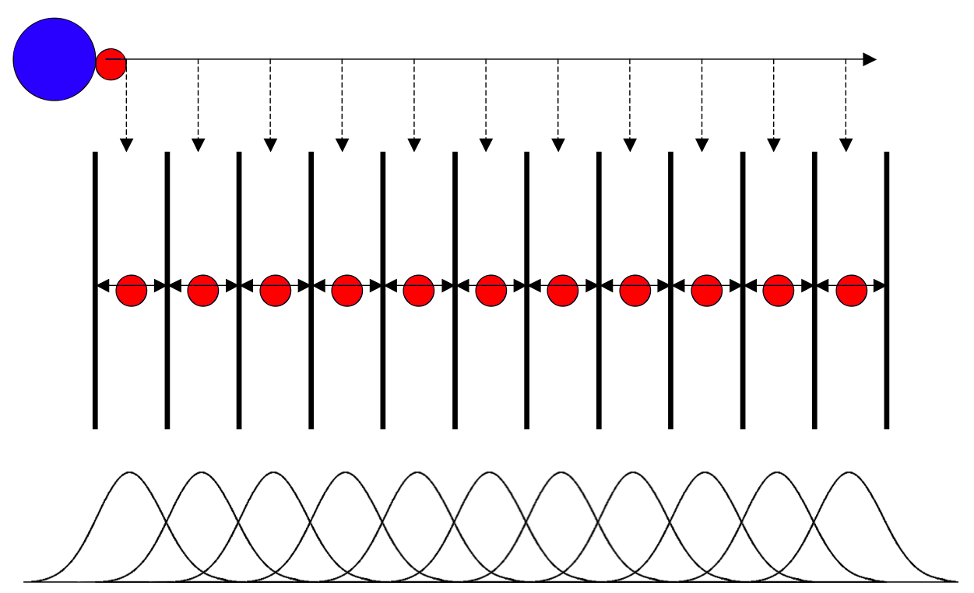
\includegraphics{umbrella_schematic2}
\caption{The process of umbrella sampling. From an initial ensemble of configurations along a reaction coordinate, several are chosen for independent simulations at intervals along the reaction coordinate. These simulations are subsequently carried out under the influence of a harmonic biasing potential, restricting their motion along the reaction coordinate to generate a restrained ensemble within a sampling window. Distributions of reaction coordinate values within each window are the "umbrellas" from which the name of the technique is derived.}
\label{umbrella_schematic_fig}
\end{figure}

To generate a series of configurations that can serve as input into the individual sampling windows, the "pull code" in GROMACS (so named for its ability to apply a biasing potential that "pulls" along a specified vector) will be employed to cause the dissociation of chain A from the remainder of the protofibril. First, create an index group for each of these chains:

\begin{lstlisting}
$ gmx make_ndx -f npt.gro
> r 1-27
> name 19 Chain_A
> r 28-54
> name 20 Chain_B
> q
\end{lstlisting}

The relevant pull code settings are listed here:

\begin{lstlisting}
pull                    = yes
pull_ncoords            = 1
pull_ngroups            = 2
pull_coord1_groups      = 1 2
pull_group1_name        = Chain_A
pull_group2_name        = Chain_B
pull_coord1_type        = umbrella
pull_coord1_geometry    = distance
pull_coord1_dim         = N N Y
pull_coord1_start       = yes
pull_coord1_rate        = 0.01
pull_coord1_k           = 1000
\end{lstlisting}

The \texttt{define = -DPOSRES\_B} line in the \texttt{.mdp} file specifies that peptide chain B is to be restrained during this process. Application of restraints here models the stability of amyloid fibrils, which are orders of magnitude larger and therefore more resilient to dissociation of terminal peptides, and also enables more efficient dissociation of chain A. In the absence of position restraints, the entire pentameric protofibril responds to the imaginary spring, causing it to diffuse through the box, distort, and ultimately not produce the desired result. In general, such position restraints are not necessary, and are rarely employed in the case of, {\em e.g.} protein-ligand or membrane systems. The application of restraints is thus somewhat unique to the system considered here and should not be viewed as generally applicable.

The \texttt{pull} keyword tells \texttt{grompp} to read settings related to the pull code. If set to \texttt{no}, all following settings (\texttt{pull\_*}) are ignored. The \texttt{pull\_ncoords} keyword specifies how many reaction coordinates will be present in the simulated system. This number can be set to any value, that is, a multi-dimensional free energy surface can be constructed in any number of dimensions. For this example, there is only one reaction coordinate, which is defined by two groups of atom selections (\texttt{pull\_ncoords = 2}). Next, the groups themselves are specified. Each of the groups is assigned an integer (1 through N, where N is the value of \texttt{pull\_ngroups}), which are subsequently named with the \texttt{pull\_groupN\_name} keyword. Here, two groups are specified by the names assigned above in the index file.

The next settings define the type of biasing potential to be applied. The \texttt{pull\_coord1\_type} specifies a harmonic biasing potential with the keyword \texttt{umbrella}. It is important to note here that, despite the name of this setting, the current process is not umbrella sampling. The \texttt{umbrella} specification is simply a synonym for the harmonic potential that is typically employed during umbrella sampling (see below, Section~\ref{umbrella_us}). The reaction coordinate itself is then specified with the \texttt{pull\_coord1\_geometry} and \texttt{pull\_coord1\_dim} settings. In this case, the \texttt{distance} between chains A and B defines the geometry of the reaction coordinate, and the biasing potential only acts along the $z$-axis (\texttt{pull\_coord1\_dim = N N Y}), which specifies the dimensions (x, y, z) and whether or not the biasing potential acts (N = no, Y = yes). The initial value of the reaction coordinate is set very simply with \texttt{pull\_coord1\_start = yes}, such that \texttt{grompp} sets the initial value to whatever is computed from the input coordinate file. One can override this value with \texttt{pull\_coord1\_init}, which specifies a floating-point number as the initial (or reference) value of the reaction coordinate.

Finally, the harmonic biasing potential parameters are set. The \texttt{pull\_coord1\_rate} setting specifies the rate at which the imaginary spring connecting the two restrained groups is extended, in nm ps\textsuperscript{-1}. The stiffness of the spring is set with \texttt{pull\_coord1\_k}, according to Hooke's Law. It is important to note that the rate of extension of the spring is not necessarily equivalent to the rate of observed displacement of the pulled groups. The imaginary spring counteracts the attractive forces in the system, and builds up until these restoring forces are overcome. This concept will be explored below in the analysis of the SMD simulation.

Use the \texttt{md\_pull.mdp} input file to prepare the input for the SMD simulation, and carry it out with \texttt{mdrun}:

\begin{lstlisting}
$ gmx grompp -f md_pull.mdp -c npt.gro -p topol.top -r npt.gro -n index.ndx -t npt.cpt -o pull.tpr

$ gmx mdrun -deffnm pull
\end{lstlisting}

\begin{figure}[ht!]
\centering
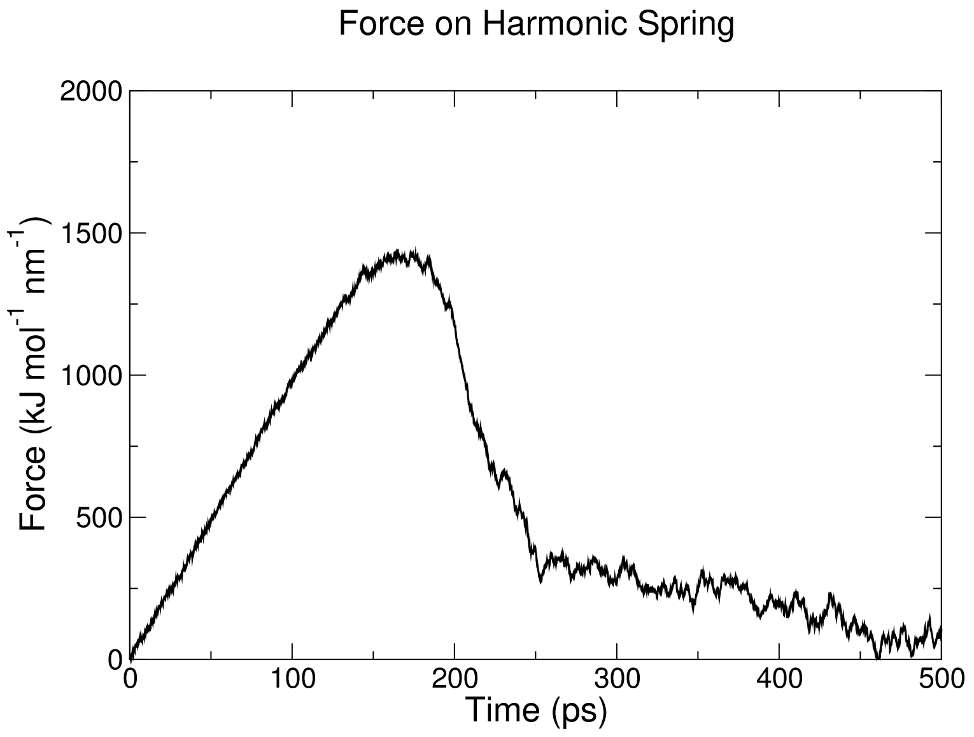
\includegraphics{umbrella_smd_pullf}
\caption{The force on the harmonic spring during SMD separation of chains A and B.}
\label{umbrella_smd_pullf_fig}
\end{figure}

After the SMD simulation is finished, plot the contents of \texttt{pullf.xvg} (Figure~\ref{umbrella_smd_pullf_fig}). This file contains the force on the imaginary spring as a function of time. Visualize the trajectory and note that chain A does not dissociate from chain B for some time. Only after the force builds up on the spring does this dissociation begin. The A$\beta$\textsubscript{42} protofibril is stabilized by extensive inter-peptide side-chain packing and backbone hydrogen bonding. Thus, a large force is required to disrupt all of these interactions, which are described in detail elsewhere~\cite{Lemkul2010}.

The \texttt{pullx.xvg} file contains the length of the reaction coordinate as a function of time. It may be useful to plot the restraint forces as a function of displacement rather than as a function of time. To extract this information, use standard Linux commands \texttt{grep} and \texttt{awk}:

\begin{lstlisting}
$ grep -v [@#] pullf.xvg | awk '{print $2}' > forces
$ grep -v [@#] pullx.xvg | awk '{print $2}' > x
$ paste x forces > pull_force_vs_displacement.xvg
$ rm x forces
\end{lstlisting}

These data are plotted in Figure~\ref{umbrella_pullf_vs_pullx_fig}.

\begin{figure}[h!]
\centering
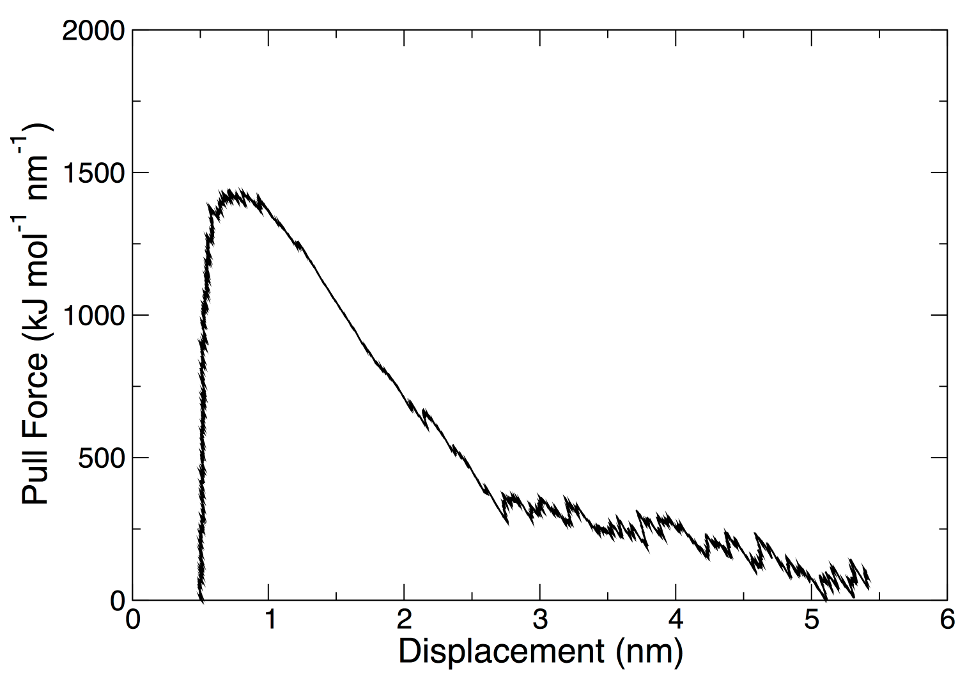
\includegraphics{umbrella_pullf_vs_pullx}
\caption{The force on the harmonic spring as a function of displacement during SMD.}
\label{umbrella_pullf_vs_pullx_fig}
\end{figure}

Next, configurations must be extracted from the trajectory to define the starting points for each of the umbrella sampling windows. There are several ways to approach this problem, and here the approach will be to:

\begin{enumerate}
	\item Write configurations of each snapshot
	\item Compute the COM distance between chains A and B in each snapshot
	\item Compile these COM distances as a function of snapshot index
	\item Use selected frames as input into umbrella sampling
\end{enumerate}

The GROMACS \texttt{trjconv} program has an option to write each frame in a trajectory to a separate file, \texttt{-sep}. Save these separate snapshots with:

\begin{lstlisting}
$ gmx trjconv -s pull.tpr -f pull.xtc -o conf.gro -sep
\end{lstlisting}

Each snapshot will be written to a file called \texttt{confN.gro}, where N is the index of the frame. The COM distance between chains A and B in each of these frames is computed with the GROMACS \texttt{distance} program, {\em e.g.} for the frame at t = 0 ps:

\begin{lstlisting}
$ gmx distance -s pull.tpr -f conf0.gro -select 'com of group "Chain_A" plus com of group "Chain_B"' -n index.ndx -oall dist0.xvg
\end{lstlisting}

Note the use of single quotes (') to enclose the entire selection string and double quotes (") to enclose group names referenced from \texttt{index.ndx}.

The online version of this tutorial provides a Bash script (\texttt{get\_distances.sh}) that automates this entire process and compiles the COM distances into a single text file. This file should be inspected for snapshots at intervals of approximately 0.2 nm (perfectly even spacing is unlikely) and the frame indices should be recorded and corresponding coordinate files saved.

It is worth noting that the COM distance as a function of time can be directly calculated from the trajectory file (\texttt{pull.xtc}) for later inspection. After this analysis, the user would have to decide which frames to extract from the trajectory and invoke \texttt{trjconv} for each of these frames. As such, the approach taken in this tutorial, while somewhat redundant, may actually be viewed as more efficient. The user can move or copy the desired frames to a new location and simply delete the unnecessary snapshots, ultimately saving time.

While the reaction coordinate in this system is straightforward and justified based on a number of experiments and other mathematical models, the general application of SMD to generate configurations may yield non-equilibrium states that are sensitive to the chosen path. When using this approach in other systems, users should be forewarned that they should generate multiple pulling vectors to generate a sufficient ensemble of potential starting states, and to equilibrate thoroughly to reasonably ensure that the path sampled is the minimum free-energy path.

\subsubsection{Umbrella Sampling} \label{umbrella_us}

Once suitable snapshots have been identified, each umbrella sampling window will be prepared. Each window is equilibrated under an $NPT$ ensemble for 100 ps before data collection is carried out over 10 ns. The COM pull settings are the same as what are shown above for the SMD simulation, with the exception of \texttt{pull\_coord1\_rate}, which is now set to zero. During these simulations, the COM distance between chains A and B is to be restrained; no net displacement is to be imposed, which is what a non-zero value of \texttt{pull\_coord1\_rate} specifies.

Prepare the input \texttt{.tpr} files for each $NPT$ equilibration and carry out those simulations (assuming that snapshot 6 corresponds to a value of $\xi$ = 0.5 nm):

\begin{lstlisting}
$ gmx grompp -f npt_umbrella.mdp -c conf6.gro -r conf6.gro -p topol.top -n index.ndx -o npt0.tpr

$ gmx mdrun -deffnm npt0
\end{lstlisting}

After equilibration, production umbrella sampling MD simulations are performed:

\begin{lstlisting}
$ gmx grompp -f md_umbrella.mdp -c npt0.gro -t npt0.cpt -p topol.top -r npt0.gro -n index.ndx -o umbrella0.tpr

$ gmx mdrun -deffnm umbrella0
\end{lstlisting}

\subsubsection{Data Analysis} \label{umbrella_analysis}

To compute the PMF along the reaction coordinate, the Weighted Histogram Analysis Method (WHAM)~\cite{Kumar1992} is employed, implemented in GROMACS as the \texttt{wham} program~\cite{Hub2010}, which also includes algorithms to estimate errors associated with the resulting PMF. From the biased simulations (sampling windows), a histogram is constructed, $h(\xi)$. This histogram describes the probability of finding the system at individual locations along the reaction coordinate, {\em i.e.} a biased probability distribution, $P_b(\xi)$. The WHAM algorithm uses $h(\xi)$ to estimate the uncertainty in an unbiased $P(\xi)$ by iteratively solving a system of equations to compute the PMF that has the smallest uncertainty. The PMF produced in this analysis corresponds to the free energy along $\xi$.

The input to the GROMACS \texttt{wham} program comprises two text files, which list the input \texttt{.tpr} file names and either the \texttt{pullf.xvg} or \texttt{pullx.xvg} files. These lists of file names are provided in two plain-text files, created with any plain-text editor. It is important that these text files contain the list of relevant files in the order they should be assembled. Create a file called \texttt{tpr-files.dat} that contains:

\begin{lstlisting}
umbrella0.tpr
umbrella1.tpr
...
umbrella22.tpr
\end{lstlisting}

Then, create a file called \texttt{pullf-files.dat} that contains:

\begin{lstlisting}
umbrella0_pullf.xvg
umbrella1_pullf.xvg
...
umbrella22_pullf.xvg
\end{lstlisting}

The ellipses in both of the above blocks of text indicate that the intervening file names should similarly be specified. Next, invoke \texttt{wham} to compute the PMF:

\begin{lstlisting}
$ gmx wham -it tpr-files.dat -if pullf-files.dat -o -hist -unit kCal
\end{lstlisting}

The above command computes a PMF in the units of kcal mol\textsuperscript{$-$1} and writes it to a file called \texttt{profile.xvg}. The corresponding umbrella histograms, $h(\xi)$, are also produced (\texttt{histo.xvg}). These results are plotted in Figure~\ref{umbrella_composite_pmf_histo_fig}.

\begin{figure}[h!]
\centering
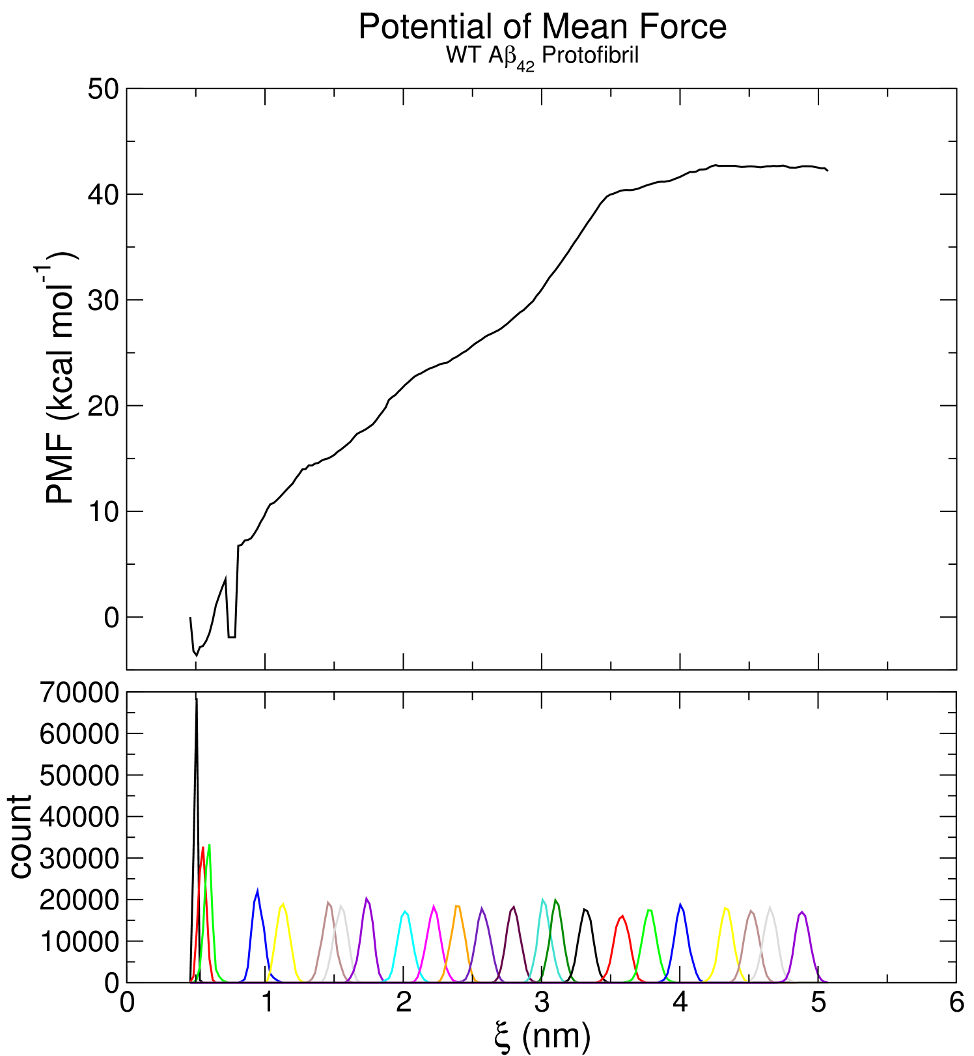
\includegraphics{umbrella_composite_pmf_histo}
\caption{The PMF computed by the WHAM algorithm and the corresponding umbrella histograms.}
\label{umbrella_composite_pmf_histo_fig}
\end{figure}

Note that \texttt{histo.xvg} is contains multiple data series and should be plotted in XmGrace as such:

\begin{lstlisting}
$ xmgrace -nxy histo.xvg
\end{lstlisting}

The PMF has an energy minimum at approximately 0.5 nm, which is the distance corresponding to inter-C$\alpha$ spacing in canonical $\beta$-sheets. The position of this minimum makes sense. The resulting $\Delta$G for dissociation is approximately 46 kcal mol\textsuperscript{$-$1}, which is close to our published value of 50.5 kcal mol\textsuperscript{$-$1}~\cite{Lemkul2010}. The difference can be attributed to the use of a different starting structure (as noted above) and different sampling window intervals. Note, however, the large defect in the PMF around 0.8 nm and the corresponding lack of sampling in the umbrella histograms in this region of the reaction coordinate (Figure~\ref{umbrella_composite_pmf_histo_fig}). This outcome indicates that this region of the reaction coordinate has not been adequately sampled and at least one more simulation must be performed. At $\xi$ = 0.8 nm, the pulling force in SMD was at its maximum (Figure~\ref{umbrella_pullf_vs_pullx_fig}), indicating that the interactions in at this $\xi$ value are very strong and this state may reflect a very high-energy intermediate that is rarely visited. In the umbrella sampling windows employed here, only $\xi$ = 0.7 nm and $\xi$ = 0.9 nm were chosen, and neither sampled around 0.8 nm. To refine this region of the PMF profile, a new simulation should be carried out at $\xi$ = 0.8 nm. The fact that umbrella sampling simulations are independent makes doing so reasonable. The existing simulations do not need to be re-run, as neighboring windows do not depend on one another, unlike other alchemical free energy methods (see Section~\ref{fes}) or enhanced sampling techniques like replica exchange.

It is also worth mentioning how WHAM computes the actual PMF values along $\xi$. By convention, the leftmost window ({\em i.e.} lowest value of $\xi$) is assigned a free energy value of zero. The energies in subsequent windows are all defined relative to this value. It may be more useful to shift some physically relevant or otherwise convenient point to zero. Such a practice does not change the result at all, it is a systematic translation of the PMF curve and the final value of $\Delta$G is the same. The GROMACS \texttt{wham} program has the ability to shift the final PMF curve to place the zero point at a user-defined location. For example, the place the zero point at the energy minimum ($\xi$ = 0.5 nm), invoke \texttt{wham} as follows:

\begin{lstlisting}
$ gmx wham -it tpr-files.dat -if pullf-files.dat -o profile_shift.xvg -hist -unit kCal -zprof0 0.5
\end{lstlisting}

The result of this new calculation is shown in Figure~\ref{umbrella_pmf_shift_fig}.

\begin{figure}[h!]
\centering
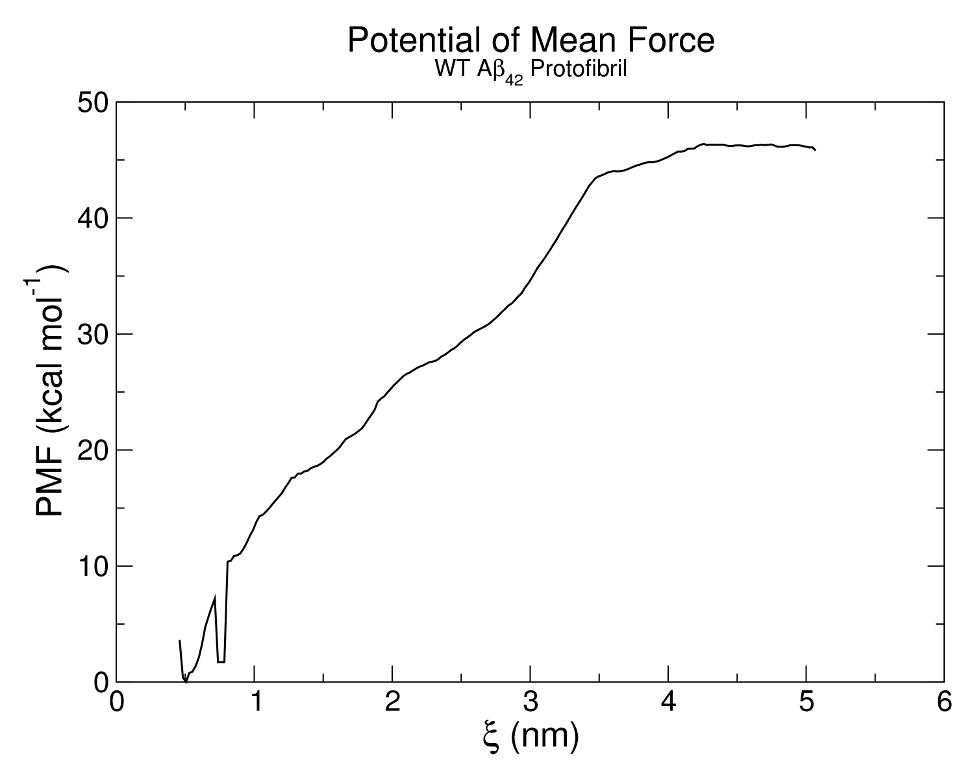
\includegraphics{umbrella_pmf_shift}
\caption{The PMF computed by the WHAM algorithm, with the zero point set to $\xi$ = 0.5 nm, the energy minimum of the profile.}
\label{umbrella_pmf_shift_fig}
\end{figure}

\subsubsection{Summary and Review of Objectives} \label{umbrella_summary}

In this tutorial, the user has been guided through the process of performing an SMD simulation of one A$\beta$\textsubscript{42} peptide from a pentameric protofibril. From the SMD trajectory, defining a one-dimensional reaction coordinate, snapshots were extracted at roughly regular intervals. These snapshots were subjected to additional equilibration and extended simulations to compute a PMF profile, which yields $\Delta$G for dissociation of the peptide. To review, the objectives for this tutorial were:

\begin{enumerate}
	\item Apply \texttt{.mdp} keywords that invoke the pull code to add a simple, one-dimensional biasing potential to selected atoms in a system
	\item Define what is meant by a "reaction coordinate" and how to construct a suitable one
	\item Perform restrained simulations in multiple sampling windows along a reaction coordinate
	\item Compute a potential of mean force profile
\end{enumerate}

In Section~\ref{umbrella_smd}, the GROMACS pull code keywords were introduced and the definition of the reaction coordinate was explained in the context of these settings. In subsequent sections, umbrella sampling calculations were performed and the WHAM algorithm~\cite{Kumar1992} was used to de-bias the histograms to compute the PMF.

To conclude, it is again important to emphasize that the system simulated here involves special considerations, including the use of position restraints and the fact that the reaction coordinate was one-dimensional. Restraints served two specific purposes: first, to allow efficient dissociation of two strongly interacting species and second, to mimic the stability of A$\beta$ fibrils that are orders of magnitude larger (heavier) than the relatively small pentamer considered here. Such restraints are not typically necessary in different systems, such as protein-ligand complexes or those involving membranes. Additionally, the growth of A$\beta$ fibrils is unidirectional, meaning that orthogonal dimensions (here, $x$ and $y$) are not relevant to the fibril association/dissociation equilibrium. Hence, the reaction coordinate can conveniently be defined along only the $z$-axis, which also allows for the user of a relatively small box, extended only along the $z$-axis beyond what is necessary to satisfy the particle-particle minimum image convention. If the system being considered is a protein-ligand complex, no such assumption can be made, the biasing force should be applied along a vector in all three spatial dimensions, and the box should be sufficiently large in all dimensions. Other, special cases may similarly be unidirectional, but this case should not be considered a default assumption. The user must always consider the intrinsic geometry or symmetry of the system being studied. As such, the \texttt{.mdp} files provided with this tutorial should be adapted for use in any other system, not used directly.



%%%%%%%%% TUTORIAL 4 %%%%%%%%%
\subsection{Tutorial 4: Biphasic Systems} \label{biphasic}

\begin{figure}[h]
\centering
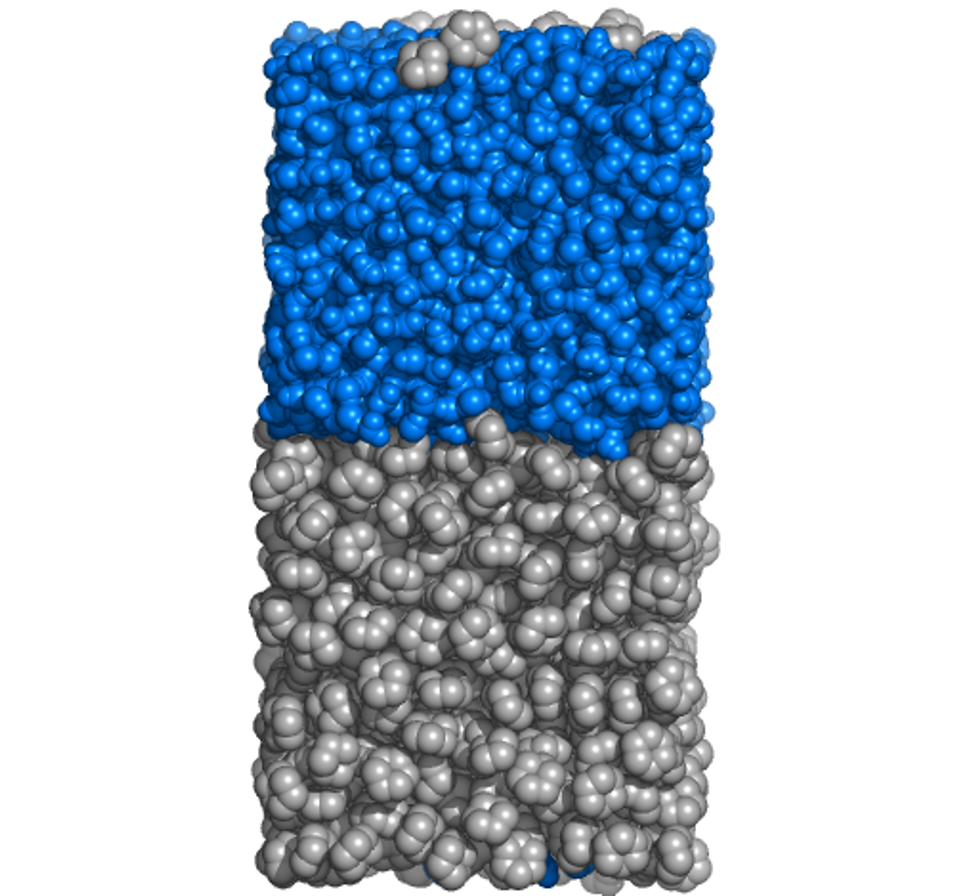
\includegraphics{biphasic_system}
\caption{A layered, biphasic system of water (blue, top) and cyclohexane (gray, bottom).}
\label{biphasic_system_fig}
\end{figure}

Heterogenous systems are often of interest in molecular simulations. For example, partitioning of a small molecule between aqueous and octanol phases is an experimentally useful property for understanding potential drug-like properties. Simulating such a process to calculate the associated change in free energy is important and may serve as a strict evaluation of force field quality. As such, the ability to construct such a system is of great importance, though it may not be apparent exactly how to do so. In this tutorial, a simple biphasic system will be constructed, containing an aqueous phase and a hydrophobic (cyclohexane) phase (Figure~\ref{biphasic_system_fig}). This tutorial will focus solely on construction of the system rather than performing and analyzing simulations. The process for simulating biphasic systems is no different from any other simulation, with perhaps the only specific consideration being the treatment of COM motion removal groups. Refer to Section~\ref{kalp_equil} for discussion on how to treat layered systems and appropriately set the \texttt{comm-grps} keyword in \texttt{.mdp} files.

The basis of this tutorial (online at \tutorialbiphasic) is a recent paper~\cite{Lemkul2010b} that explored small-molecule and amino-acid dynamics at a water-cyclohexane interface, to test the behavior of the GROMOS96 43A1 force field~\cite{Daura1998,Schuler2001} and topologies produced by the PRODRG server~\cite{vanAalten1996}.

\subsubsection{Build a Cyclohexane Box} \label{biphasic_chx_box}

To begin, the user needs a coordinate file containing a single cyclohexane molecule and a corresponding topology. Coordinates can be obtained from a number of different model-building programs, but the topology has to be generated, which requires advance knowledge of its parameters or some method to derive them. A simple method to obtain both coordinates and topology for use with GROMOS force fields are online servers PRODRG~\cite{vanAalten1996} and ATB~\cite{Malde2011}. The online version of this tutorial provides suitable coordinate and topology files. Note that if the user obtains a topology from PRODRG, the partial charges in the topology should all be corrected to zero, as required by the united-atom treatment of CH\textsubscript{2} groups.

There are two methods in GROMACS by which a user can build a box of pure liquid. The first uses the \texttt{insert-molecules} program to randomly insert a specified number of molecules into a box of given dimensions. Note that this approach does not guarantee that all requested molecules will be added, rather the user specifies a maximum number to be added. The output should always be inspected to ensure that the volume is adequately filled.

To build a 5-nm cubic box and attempt to fill it with up to 1200 cyclohexane molecules, invoke \texttt{insert-molecules}:

\begin{lstlisting}
$ gmx insert-molecules -ci chx.gro -nmol 1200 -box 5 5 5 -o chx_box.gro
\end{lstlisting}

The program reports that 1114 of the requested 1200 cyclohexane molecules were placed in the box. Note that default van der Waals radii used by GROMACS programs like \texttt{insert-molecules} and \texttt{solvate} were changed in version 5.0, so different versions may report different outcomes with respect to this number. As insertion is randomly seeded process, even versions in the 2018.x series may vary slightly.

The second method for constructing a box of pure liquid uses the \texttt{genconf} program to build a lattice of molecules. This approach requires that the input coordinate file have a properly defined periodic box size so that molecules can be positioned correctly without overlapping. If the box size is not adequate, the \texttt{-dist} option (which takes a full vector as its argument) can be used to space the replicated coordinates. The drawback to the \texttt{genconf} method is that the resulting system is highly artificial because it is a perfect lattice, and will require a much longer equilibration time to converge to a liquid state. To build a box containing 512 cyclohexane molecules (8\textsuperscript{3}), invoke \texttt{genconf} as follows:

\begin{lstlisting}
$ gmx genconf -f chx.gro -nbox 8 8 8 -o chx_box.gro
\end{lstlisting}

Regardless of the method of preparing the cyclohexane box, these initial coordinates are either random or highly ordered, requiring energy minimization and subsequent equilibration. The online version of the tutorial provides an equilibrated box of 466 cyclohexane molecules in a 4.3-nm box prepared by $NVT$ and $NPT$ equilibration at 298 K, the latter phase lasting for 10 ns. It is this box that will be used for subsequent preparation steps in this tutorial. The online tutorial also provides a system topology, \texttt{chx.top}, corresponding to this system.

\subsubsection{Add a Water Layer} \label{biphasic_water}

At this point, the cubic cyclohexane box could simply be centered within a new, tetragonal box that is extended along one spatial dimension and the empty volume filled with water. The resulting system would have cyclohexane-water interfaces within the central unit cell, and the water layer would be continuous due to PBC. While perfectly viable from the perspective of physics, such a setup is somewhat inconvenient if the user is attempting to add other species (solutes, peptides, etc.) into one of the layers. As such, it is equivalent and perhaps more intuitive to position the existing cyclohexane coordinates in an elongated box such that both the water and cyclohexane layers are contiguous within the central periodic image.

As in the Umbrella Sampling tutorial (see Section~\ref{umbrella_box}), set the existing coordinates at their previous position within the newly extended box using \texttt{editconf}. The cyclohexane box is a 4.30795-nm cube, meaning its geometric center is located at (2.153975, 2.153975, 2.153975). Double the box length along the $z$-axis and retain this geometric center:

\begin{lstlisting}
$ gmx editconf -f chx_10ns.gro -o chx_newbox.gro -box 4.30795 4.30795 8.6159 -center 2.153975 2.153975 2.153975
\end{lstlisting}

The resulting system will look like what is shown in Figure~\ref{biphasic_system_newbox_fig}.

\begin{figure}[h!]
\centering
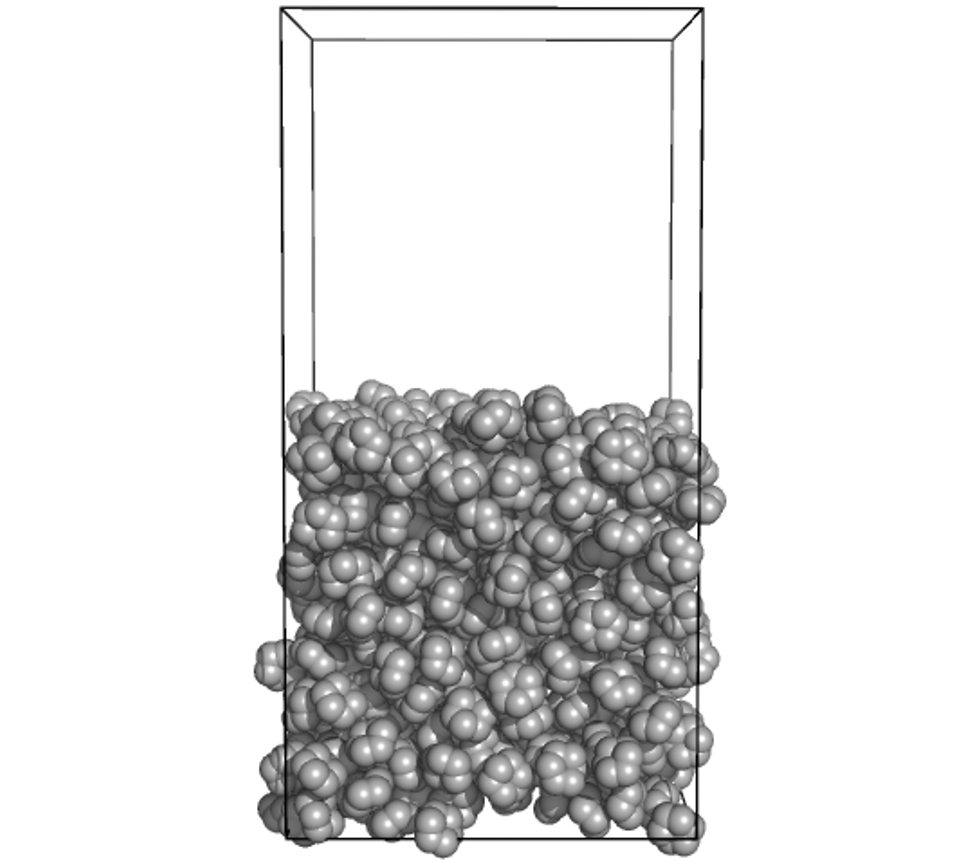
\includegraphics{biphasic_system_newbox}
\caption{The equilibrated cyclohexane box is repositioned within a tetragonal unit cell that is elongated along the $z$-axis.}
\label{biphasic_system_newbox_fig}
\end{figure}

The next step is to solvate the empty volume with water. There are likely to be small voids within the cyclohexane layer into which water will be added by the \texttt{solvate} program, so make a copy of \texttt{vdwradii.dat} from \texttt{\$GMXLIB} into the working directory. Change the default value of the C radius from 0.17 to 0.35, then run \texttt{solvate}:

\begin{lstlisting}
$ gmx solvate -cp chx_newbox.gro -cs spc216.gro -p chx.top -o chx_solv.gro
\end{lstlisting}

There are likely to be a few stray water molecules within the cyclohexane layer, even with this large radius assigned to C atoms. These waters will be expelled quickly in a short equilibration run. Water molecules appearing at the "bottom" of the box are no concern, as they are actually continuous with the water layer in the central image via the periodic boundary along the {\em z}-axis. The biphasic system is now constructed and ready for energy minimization and subsequent MD simulation.

\subsubsection{Other Tips and Tricks} \label{biphasic_tips_tricks}

To study partitioning behavior of peptides or small molecules, the approach taken in this tutorial can be expanded to position any other species within the aqueous layer prior to solvation. Similarly, the equilibrated cyclohexane box can be used as input to \texttt{solvate -cs} to place a solute in the hydrophobic layer. To add something to the aqueous layer, apply the same concepts as in the previous section to specify its center with \texttt{editconf}. This time, the center of the molecule along the $z$-axis is three-quarters of the box length. For example, to add the KALP\textsubscript{15} peptide from the Membrane Protein tutorial (see Section~\ref{kalp}) in the aqueous layer, at the center of the empty volume:

\begin{lstlisting}
$ gmx editconf -f peptide.gro -o peptide_newbox.gro -box 4.30795 4.30795 8.6159 -center 2.153975 2.153975 6.461925
\end{lstlisting}

Then "solvate" the peptide with the repositioned cyclohexane layer, which has box dimensions identical to what were just assigned to the peptide, meaning the two components will fit together exactly:

\begin{lstlisting}
$ gmx solvate -cp peptide_newbox.gro -cs chx_newbox.gro -o peptide_chx.gro
\end{lstlisting}

The resulting system appears in Figure~\ref{peptide_chx_fig}, and can subsequently be solvated with water using \texttt{solvate}.

\begin{figure}[h!]
\centering
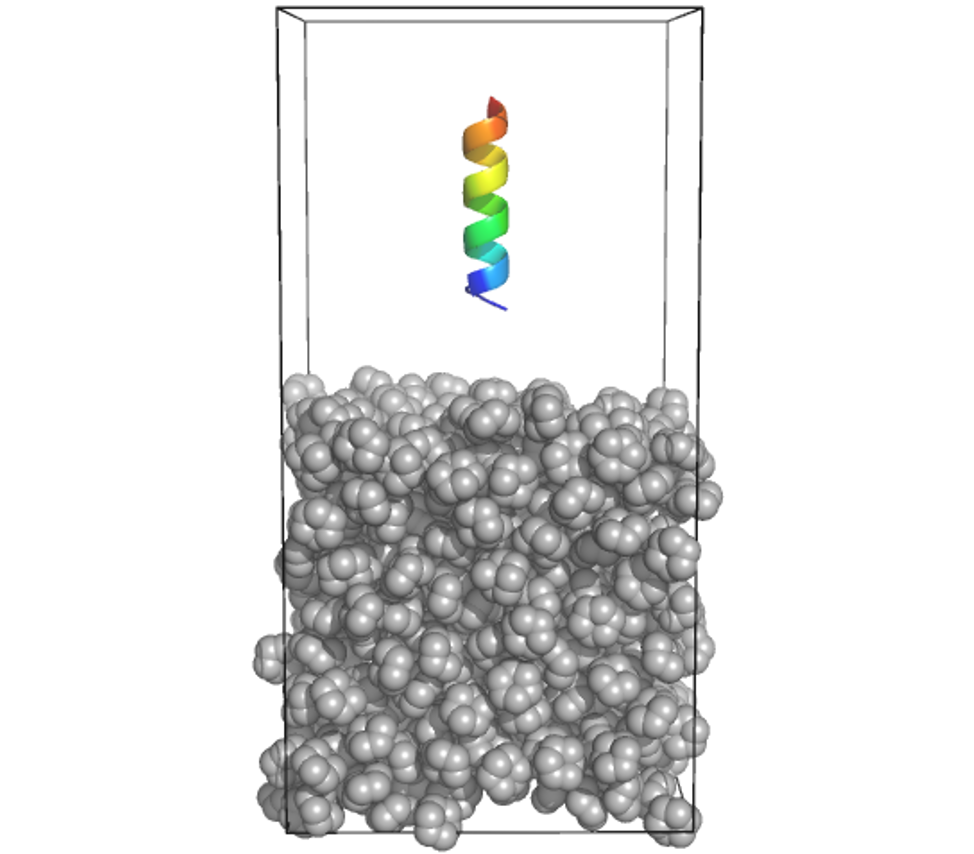
\includegraphics{peptide_chx}
\caption{The KALP\textsubscript{15} peptide has been positioned at the middle of the empty volume that will subsequently be filled with water.}
\label{peptide_chx_fig}
\end{figure}

Should a larger volume be necessary to accommodate larger molecules in the aqueous phase, the cyclohexane layer can be expanded using the GROMACS \texttt{genconf} program. The existing cyclohexane coordinates can be expanded in any number of copies along any of the three spatial dimensions. To build a larger cubic box of cyclohexane:

\begin{lstlisting}
$ gmx genconf -f chx_10ns.gro -nbox 2 2 2 -o chx_bigbox.gro
\end{lstlisting}

In the event that a tetragonal layer is necessary, do not replicate along the $z$-axis, only through the $x-y$ plane:

\begin{lstlisting}
$ gmx genconf -f chx_10ns.gro -nbox 2 2 1 -o chx_biglayer.gro
\end{lstlisting}

\subsubsection{Summary and Review of Objectives} \label{biphasic_summary}

This tutorial has guided the user through the simple construction of a biphasic system containing two layers: water and cyclohexane. The logic applied here can be used in any similar systems. To review, the learning objectives of the tutorial are:

\begin{enumerate}
	\item Build a simulation system containing a liquid that is not water
	\item Manipulate the relative positioning of a box within a larger volume
\end{enumerate}

The tutorial demonstrated how an initial system of non-aqueous liquid can be built by two different methods, and subsequently how the equilibrated box can have its relative position manipulated within a new, larger unit cell. Additional tips and tricks have been provided to demonstrate how other species can easily be added to the biphasic system, to allow for studies of interfacial dynamics and partitioning.



%%%%%%%%% TUTORIAL 5 %%%%%%%%%
\subsection{Tutorial 5: Protein-Ligand Complex} \label{prot_lig}

\begin{figure}[h]
\centering
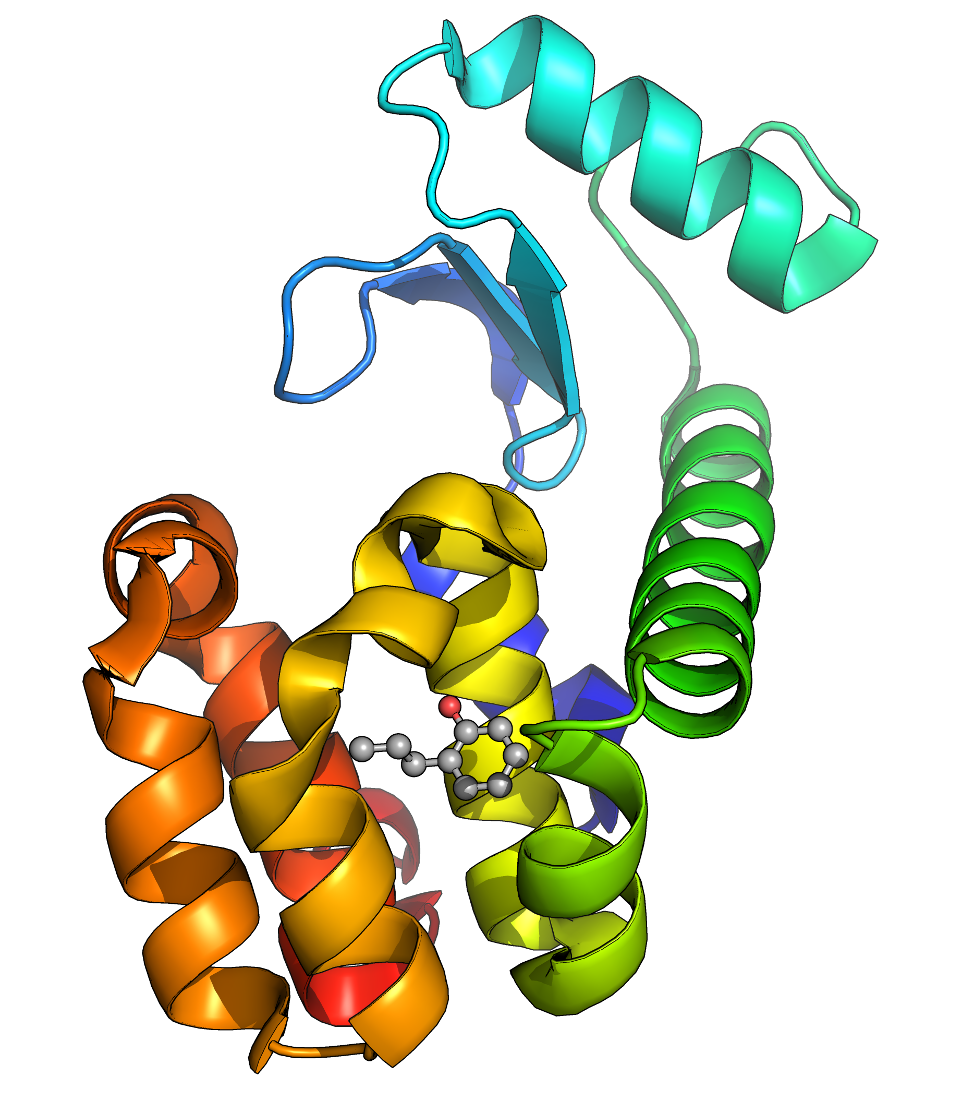
\includegraphics{lysozyme_complex_3htb}
\caption{Crystal structure of T4 lysozyme L99A/M102Q with bound 2-propylphenol ligand, taken from PDB 3HTB~\cite{Boyce2009}.}
\label{lyso_complex_3htb_fig}
\end{figure}

Simulating proteins in complex with small-molecule ligands or inhibitors (Figure~\ref{lyso_complex_3htb_fig}) is an important part of understanding enzyme catalysis, drug design, and allostery. These simulations present a challenge in that the ligand topology is not likely to have been explicitly derived. Force field parametrization is an advanced topic, one that typically requires expert training. To decrease the barrier to performing these important simulations, many "general" or "drug-like" force fields exist, such as the General AMBER Force Field (GAFF)~\cite{Wang2004}, CHARMM General Force Field (CGenFF)~\cite{Vanommeslaeghe2010}, and OPLS3~\cite{Harder2016}, which have well-known methodologies, parameter assignment protocols, and web servers that can generate topologies for arbitrary molecules.

In this tutorial (available online at \tutorialcomplex), the protein topology will be generated with the CHARMM36m force field~\cite{Huang2016}, a recent revision of the CHARMM36 force field~\cite{Best2012}. The ligand topology will be generated with CGenFF via its web server (\url{https://cgenff.paramchem.org/}). Download the CHARMM36m force field in GROMACS format from the MacKerell lab website (\url{http://mackerell.umaryland.edu/charmm_ff.shtml#gromacs}), as well as the Python script called \texttt{cgenff\_charmm2gmx.py}. Extract the force field archive in the working directory:

\begin{lstlisting}
$ tar -zxvf charmm36-jul2017.ff.tgz
\end{lstlisting}

\subsubsection{Protein Topology Preparation} \label{complex_top}

Download the coordinates for T4 lysozyme L99A/M102Q from PDB entry 3HTB. Remove crystal waters and the phosphate (PO4) and $\beta$-mercaptoethanol (BME) co-solvents from the coordinate file. The online version of the tutorial provides a file called \texttt{3HTB\_clean.pdb} that has already removed the unnecessary atoms.

The GROMACS program \texttt{pdb2gmx} can only generate topologies for species it recognizes, {\em e.g.} those encoded in residue topology (\texttt{.rtp}) files. That means non-standard species like ligands will cause the program to return a fatal error. Thus, \texttt{pdb2gmx} cannot be used to generate a topology for 2-propylphenol. It will be parametrized separately. For now, remove the atoms corresponding to the ligand (residue name JZ4) from the PDB file and save them in a separate file to be used later:

\begin{lstlisting}
$ grep JZ4 3HTB_clean.pdb > jz4.pdb
\end{lstlisting}

After saving these coordinates, delete the JZ4 coordinate lines from \texttt{3HTB\_clean.pdb} and generate the protein topology with \texttt{pdb2gmx}:

\begin{lstlisting}
$ gmx pdb2gmx -f 3HTB_clean.pdb -o 3HTB_processed.gro
\end{lstlisting}

When prompted, choose the CHARMM36 force field (the first entry in the list, "From current directory") and the default water model, TIP3P modified for use with CHARMM.

\subsubsection{Ligand Topology Preparation} \label{complex_lig_top}

The principal challenge in performing a protein-ligand simulation is generating a topology for the ligand. Most biomolecular force fields include parameters for common cofactors (heme, ATP, etc.) but do not have existing parameters for every molecule that may be of interest in a simulation. The general force fields listed above seek to remedy this situation, by establishing highly transferable atom types and parameters that can be assigned to arbitrary molecules according to established rules. Doing so removes the burden of manual parametrization from the user, as these procedures often require expert training. General force fields are not necessarily perfect, and there are instances for which manual refinement or reparametrization may be necessary, but they provide a reasonable starting point for these efforts.

In this tutorial, the CGenFF parameter set will be used to generate the topology for the 2-propylphenol ligand (Figure~\ref{jz4_fig}). CGenFF is both a parameter set (compatible with the CHARMM force field) and a program that builds small-molecule topologies according to existing rules~\cite{Vanommeslaeghe2012a,Vanommeslaeghe2012b}. The CGenFF program can be accessed via a web server (\url{https://cgenff.paramchem.org/}), which will be used in this tutorial. The input to the CGenFF program is a \texttt{.mol2} file, which contains atom names, coordinates, Tripos atom types, charges, and bonded connectivity. CGenFF uses these atom types and charges to perform its own parametrization.

\begin{figure}[h!]
\centering
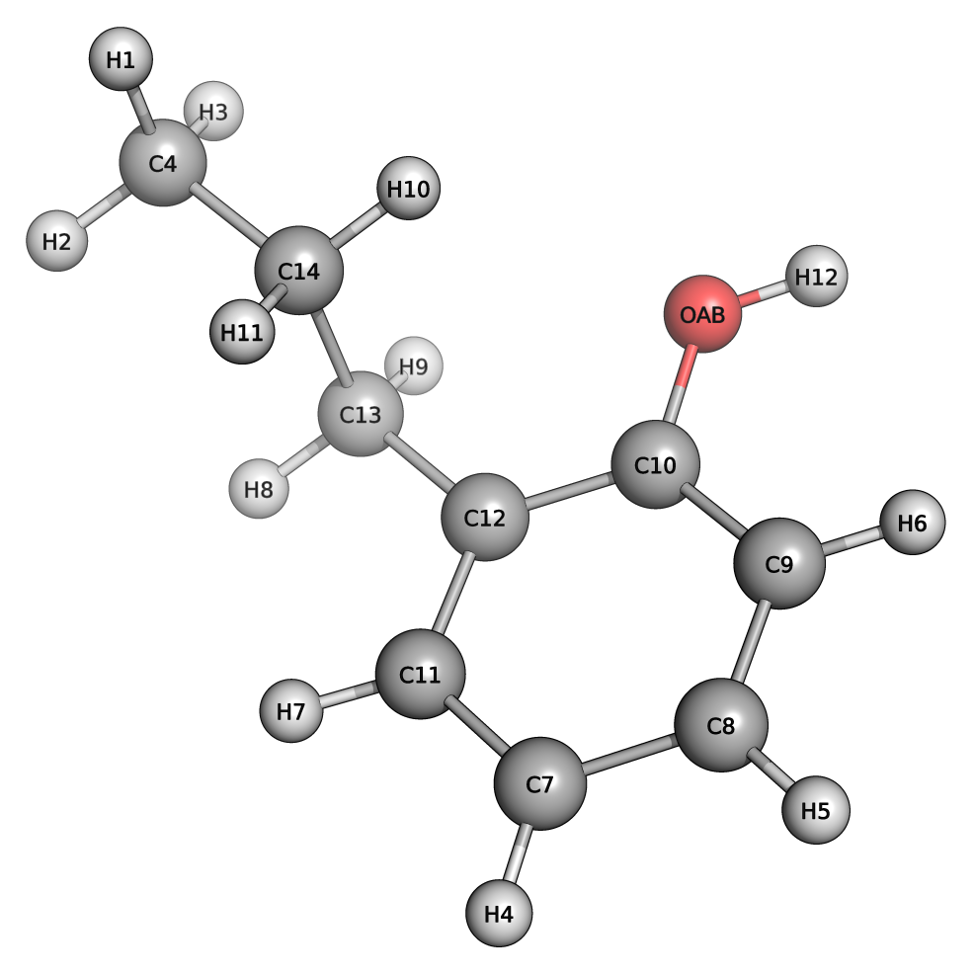
\includegraphics{jz4}
\caption{The structure of 2-propylphenol, with hydrogen atoms added. Each atom is labeled by name.}
\label{jz4_fig}
\end{figure}

To prepare the \texttt{.mol2} file, download and install the Avogadro molecular editor (\url{https://avogadro.cc/})~\cite{Hanwell2012}. Open \texttt{jz4.pdb} within Avogadro, and from the "Build" menu, choose "Add Hydrogens." Save a \texttt{.mol2} file called \texttt{jz4.mol2}. Several corrections to this file are necessary. The second line of the file, under the \texttt{@<TRIPOS>MOLECULE} heading, reads simply "*****" in place of a residue name. Replace this text with "JZ4." The hydrogen atoms that were added are assigned a different residue name and number, which must be manually corrected. Every instance of "JZ167" or "UNL1" should be replaced with "JZ4," and every atom should have a residue number of 1. The corrected \texttt{jz4.mol2} file is provided in the online version of the tutorial.

This file is syntactically valid, but still needs modification. The bonds in the \texttt{@<TRIPOS>BONDS} section do not appear in ascending numerical order, which will cause problems for CGenFF. To correct this bond listing, use the \texttt{sort\_mol2\_bonds.pl} script provided with the online tutorial:

\begin{lstlisting}
$ perl sort_mol2_bonds.pl jz4.mo2 jz4_fix.mol2
\end{lstlisting}

The final, fully corrected file \texttt{jz4\_fix.mol2} is what will be used as input to the CGenFF server.

The \texttt{jz4\_fix.mol2} will next be uploaded to the CGenFF web server. The use of this server is free for academic purposes, though user registration is required. Once \texttt{jz4\_fix.mol2} has been uploaded, the server will return a topology and parameter file in a CHARMM-formatted stream file (\texttt{jz4.str}). This file should be downloaded from the CGenFF website so it can be converted to GROMACS format. Before continuing, the contents of \texttt{jz4.str} should be inspected. CGenFF calculates penalty scores as an indicator of the quality of the topology. Parameters are assigned by analogy, and in cases for which a strong match cannot be made, the penalty score will be large. Any penalty less than 10 indicates a reliable topology. Penalties between 10 and 50 inform the user that some refinement may be necessary, and at minimum, some basic validation should be performed (QM potential energy scans in the case of bonded parameters, QM water interactions for charges), and penalty scores larger than 50 indicate that significant manual refinement or reparametrization is required. The CGenFF topology for 2-propylphenol has penalties below 1 for both charges and the new dihedrals that were generated. This topology is likely suitable for use directly as it is.

To produce a GROMACS-formatted topology, use the \\\texttt{cgenff\_charmm2gmx.py} script downloaded earlier from the MacKerell lab website. Invoke it as follows:

\begin{lstlisting}
$ python cgenff_charmm2gmx.py JZ4 jz4_fix.mol2 jz4.str charmm36-jul2017.ff
\end{lstlisting}

Recall from the introduction that this conversion script requires a Python version in the 2.7.x series, with a NetworkX version in the 1.11.x series, not the 2.x series. When finished, the conversion script will produce three important output files:

\begin{enumerate}
	\item \texttt{jz4.itp} - the topology of 2-propylphenol (JZ4) in GROMACS format
	\item \texttt{jz4.prm} - additional parameters required for the ligand topology
	\item \texttt{jz4\_ini.pdb} - the coordinates of the ligand
\end{enumerate}

To regenerate the protein-ligand complex, the coordinates of JZ4 (with hydrogen atoms added) must be appended to those of the T4 lysozyme enzyme. First, convert the \texttt{jz4\_ini.pdb} to \texttt{.gro} format:

\begin{lstlisting}
$ gmx editconf -f jz4_ini.pdb -o jz4.gro
\end{lstlisting}

Copy the enzyme coordinates from \texttt{3HTB\_processed.gro} to a new file, called \texttt{complex.gro}. Copy and paste the coordinates from \texttt{jz4.gro} into \texttt{complex.gro}, immediately after the protein coordinates and before the last line containing the box vectors. The JZ4 ligand contains 22 atoms, so add 22 to the number of protein atoms in the second line of \texttt{complex.gro}. There should be 2636 atoms in this coordinate file after the addition of the ligand coordinates.

Having added the coordinates of the ligand to the system, the topology must also be updated. Add the ligand topology to \texttt{topol.top} as shown here:

\begin{lstlisting}
; Include Position restraint file
#ifdef POSRES
#include "posre.itp"
#endif

; Include ligand topology
#include "jz4.itp"

; Include water topology
#include "./charmm36-jul2017.ff/tip3p.itp"
\end{lstlisting}

Since the ligand requires new parameters to be added to the force field, the \texttt{jz4.prm} file must also be add to the topology via an \texttt{\#include} statement. Such a statement must be placed specifically within \texttt{topol.top}. It must be after the \texttt{\#include} statement for the CHARMM36 force field, but before the declaration of the protein \texttt{[moleculetype]} directive. Bonded parameters can only be added for known atom types, hence why \texttt{jz4.prm} must be added after the first call to the CHARMM36 force field. Similarly, all parameters in the force field must be defined before any molecule definitions can be introduced. Therefore, update \texttt{topol.top} to read as follows:

\begin{lstlisting}[basicstyle=\small\ttfamily]
; Include forcefield parameters
#include "./charmm36-jul2017.ff/forcefield.itp"

; Include ligand parameters
#include "jz4.prm"

[ moleculetype ]
; Name            nrexcl
Protein_chain_A     3
\end{lstlisting}

Finally, update the contents of the \texttt{[ molecules ]} directive of \texttt{topol.top} to reflect the fact that the ligand coordinates have been added to the system:

\begin{lstlisting}[basicstyle=\small\ttfamily]
[ molecules ]
; Compound        #mols
Protein_chain_A     1
JZ4                 1
\end{lstlisting}

\subsubsection{Solvate the System} \label{complex_solv}

The remaining steps in preparing the simulation system are much like any other system of a protein in water. In this tutorial example, the protein-ligand complex will be solvated in a rhombic dodecahedral unit cell, which requires only approximately 77\% of the volume of a cubic unit cell with the same periodic distance. It is therefore more efficient to use such a box shape. Place the T4 lysozyme-JZ4 complex in a rhombic dodecahedral box with \texttt{editconf} and add water with \texttt{solvate}.

\begin{lstlisting}
$ gmx editconf -f complex.gro -o newbox.gro -bt dodecahedron -d 1.0

$ gmx solvate -cp newbox.gro -cs spc216.gro -p topol.top -o solv.gro
\end{lstlisting}

When visualized, it will appear that the protein-ligand complex has not been centered in the box and the added water appears to occupy a tetragonal unit cell. This point is often confusing for new users but should not be a concern. By default, GROMACS will re-wrap the coordinates into a triclinic box, which is the most efficient form for carrying out the necessary vector operations during a simulation. The coordinates of the solvated system and their relationship to a triclinic unit cell are shown in Figure~\ref{3htb_unit_cell_fig}. Recovering the dodecahedral box shape will be discussed later in this tutorial, but it is not necessary to make any changes to the solvated coordinates. The desired geometry will be used in the simulation.

\begin{figure}[h!]
\centering
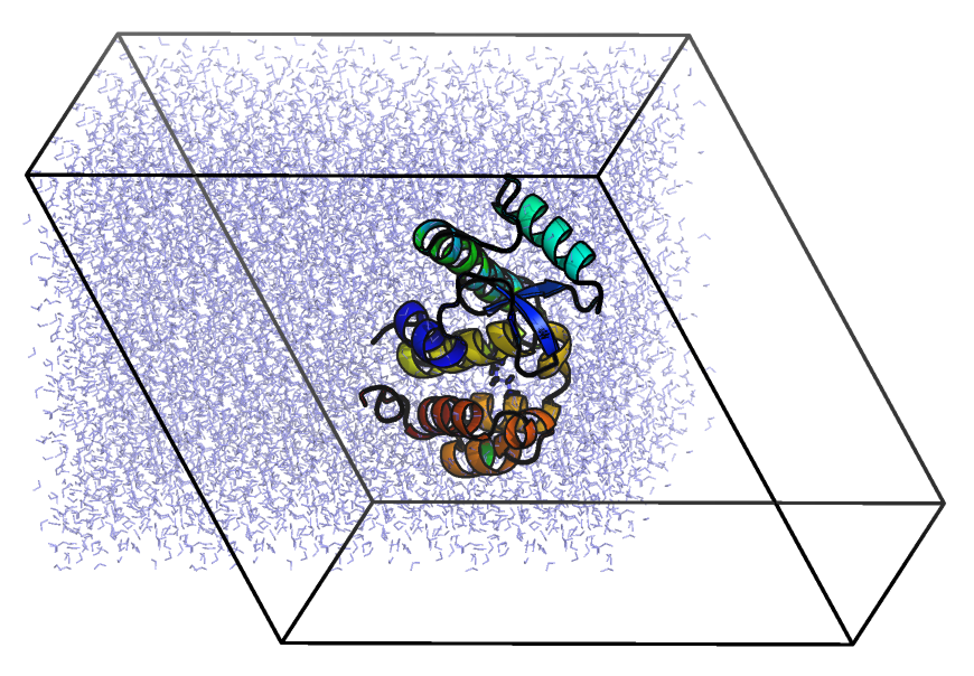
\includegraphics{3htb_unit_cell}
\caption{The coordinates of the solvated system and within a triclinic unit cell shape.}
\label{3htb_unit_cell_fig}
\end{figure}

Next, add neutralizing counterions to the system. The T4 lysozyme enzyme carries a +6 charge at neutral pH, so 6 Cl\textsuperscript{$-$} ions will be added by \texttt{genion}.

\begin{lstlisting}
$ gmx grompp -f ions.mdp -c solv.gro -p topol.top -o ions.tpr

$ gmx genion -s ions.tpr -o solv_ions.gro -p topol.top -pname NA -nname CL -neutral
\end{lstlisting}

\subsubsection{Energy Minimization and Equilibration} \label{complex_em_eq}

The solvated, neutralized system will be energy-minimized and equilibrated in two phases, $NVT$ and $NPT$, following the same protocol as the lysozyme system described above (Sections~\ref{lyso_em} and~\ref{lyso_equil}). There are notable differences in the \texttt{.mdp} files used here that warrant further explanation. The CHARMM36 force field requires the use of a switching function on the short-range forces, rather than a plain cutoff. The relevant settings are listed here:

\begin{lstlisting}
cutoff-scheme           = Verlet
ns_type                 = grid
nstlist                 = 20
rlist                   = 1.2
vdwtype                 = cutoff
vdw-modifier            = force-switch
rvdw-switch             = 1.0
rvdw                    = 1.2
\end{lstlisting}

The short-range nonbonded cutoff is set to 1.2 nm, and a buffered neighbor list is constructed with the Verlet cutoff scheme, meaning that the actual value of \texttt{rlist} will be increased as needed to conserve energy. The van der Waals forces are truncated (\texttt{vdwtype = cutoff}) at 1.2 nm (\texttt{rvdw}), with an "inner" cutoff of 1.0 nm set with \texttt{rvdw-switch}, specifying the start of a region over which the forces are smoothly switched to zero, specified by \texttt{vdw-modifier = force-switch}. This nonbonded convention is the one for which the CHARMM force field was parametrized. It is important to utilize these settings to ensure a valid simulation. Electrostatic forces are calculated with PME and a real-space cutoff of 1.2 nm.

\begin{lstlisting}
$ gmx grompp -f em.mdp -c solv_ions.gro -p topol.top -o em.tpr

$ gmx mdrun -deffnm em
\end{lstlisting}

During equilibration, the solute non-hydrogen atoms are typically restrained. In this system, the solute includes the 2-propylphenol ligand, but no restraint topology exists for it. The GROMACS \texttt{genrestr} program can be used to create such a topology, but first an index group specifying only the non-hydrogen atoms in the ligand is required. Create the index file with \texttt{make\_ndx}:

\begin{lstlisting}
gmx make_ndx -f jz4.gro -o index_jz4.ndx
> 0 & ! a H*
> q
\end{lstlisting}

The expression above (\texttt{0 \& ! a H*}) selects all atoms in the system (group 0) that do not (!) have names starting with H. Once this index file has created, use it to write a position restraint topology for the ligand, selecting group 3 when prompted.

\begin{lstlisting}
$ gmx genrestr -f jz4.gro -o posre_jz4.itp -n index_jz4.ndx -fc 1000 1000 1000
\end{lstlisting}

In Section~\ref{lyso_equil}, the concept of thermostats was introduced. The typical strategy is to assign solute and solvent atom to separate thermostatting groups. In this case, the ligand is encompassed by the default \texttt{non-Protein} group. Given that the ligand is physically bound to the protein, its dynamics are therefore coupled to those of the protein in a way that makes it illogical to include the ligand in the generic \texttt{non-Protein} group, which includes solvent. It is more logical to couple the ligand together with the protein. To do so, again invoke \texttt{make\_ndx} to merge the "Protein" and "JZ4" groups (1 and 13, respectively):

\begin{lstlisting}
$ gmx make_ndx -f em.gro -o index.ndx
...
> 1 | 13
> q
\end{lstlisting}

Then, continue with $NVT$ and $NPT$ equilibration. In each, the thermostat has two groups (\texttt{tc-grps}). One is set to the merged protein-ligand group (\texttt{Protein\_JZ4}) and the other is the solvent (\texttt{Water\_and\_ions}).

\begin{lstlisting}
$ gmx grompp -f nvt.mdp -c em.gro -r em.gro -p topol.top -n index.ndx -o nvt.tpr

$ gmx mdrun -deffnm nvt
\end{lstlisting}

\begin{lstlisting}
$ gmx grompp -f npt.mdp -c nvt.gro -t nvt.cpt -r nvt.gro -p topol.top -n index.ndx -o npt.tpr

$ gmx mdrun -deffnm npt
\end{lstlisting}

\subsubsection{Production MD Simulation} \label{complex_md}

Once equilibrated, the position restraints are released and a production MD simulation is performed. All settings in the \texttt{.mdp} file are familiar by now and need no repeating here. In this tutorial, the simulation will be carried out for 10 ns, which is still generally too short for most real purposes, but enough time to illustrate some principles of post-processing and analysis in the next section.

\begin{lstlisting}
$ gmx grompp -f md.mdp -c npt.gro -t npt.cpt -p topol.top -n index.ndx -o md_0_10.tpr

$ gmx mdrun -deffnm md_0_10
\end{lstlisting}

\subsubsection{Analysis} \label{complex_analysis}

After the simulation is over, the effects of periodic boundary conditions must be accounted for, as in Section~\ref{lyso_ana}. The GROMACS \texttt{trjconv} program is again used to perform the required coordinate manipulations. Additionally, \texttt{trjconv} allows for re-wrapping of the coordinates to recover the rhombic dodecahedral box shape. Process the MD trajectory by placing all whole molecules in the box, wrapping the coordinates into their most compact form, and centering the protein:

\begin{lstlisting}
$ gmx trjconv -s md_0_10.tpr -f md_0_10.xtc -o md_0_10_center.xtc -center -pbc mol -ur compact
\end{lstlisting}

Choose the "Protein" group for centering  and "System" for output.

To visualize the trajectory in a program like VMD, extract the first frame and save it as a coordinate file (\texttt{.gro} or \texttt{.pdb} format):

\begin{lstlisting}
$ gmx trjconv -s md_0_10.tpr -f md_0_10_center.xtc -o start.pdb -dump 0
\end{lstlisting}

It is also apparent that this coordinate file has the expected box shape (Figure~\ref{3htb_t0_rewrap_fig}).

\begin{figure}[h!]
\centering
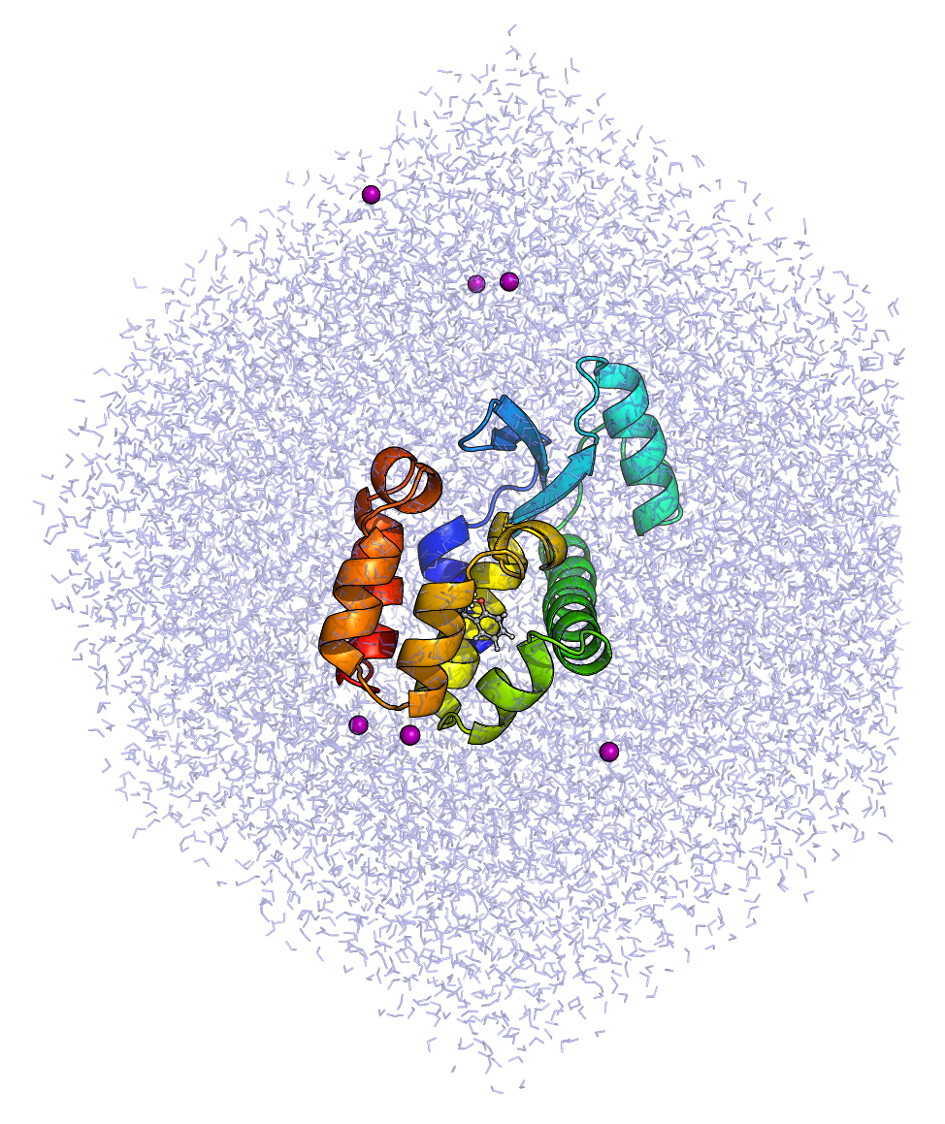
\includegraphics{3htb_t0_rewrap}
\caption{The coordinates of the solvated, equilibrated system after coordinate re-wrapping to yield the most compact box shape, the rhombic dodecahedron.}
\label{3htb_t0_rewrap_fig}
\end{figure}

To make an even smoother rendering of the trajectory, perform rotational and translational fitting. Select "Backbone" for fitting and "System" for output. Note that fitting and PBC re-wrapping cannot be performed at the same time, hence there are two calls to \texttt{trjconv} needed to perform these steps. Rotational and translational fitting via \texttt{trjconv} is not required for analysis, but can be useful for visualization, particularly for long trajectories in which the protein may diffuse substantially.

\begin{figure}[ht!]
\centering
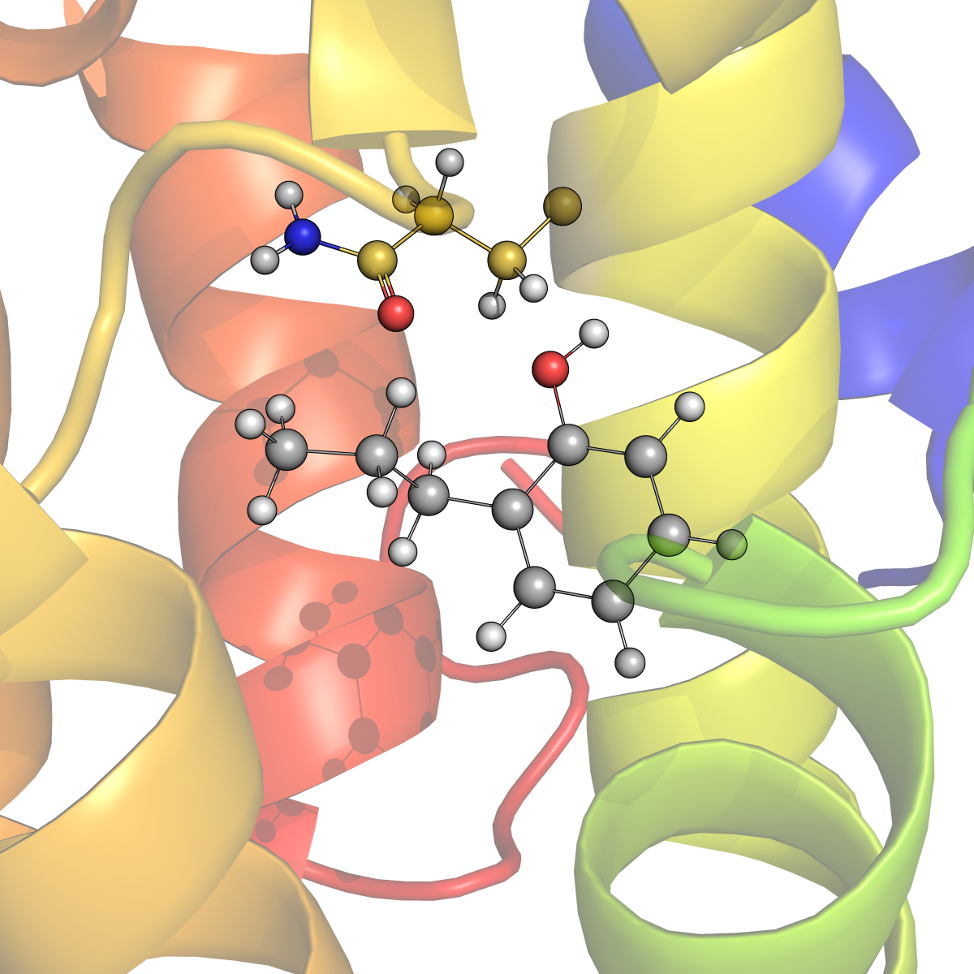
\includegraphics{3htb_jz4_zoom}
\caption{The 2-propylphenol ligand in the active site of T4 lysozyme after energy minimization, with nearby Gln102 shown in ball-and-stick rendering.}
\label{3htb_jz4_zoom_fig}
\end{figure}

\begin{lstlisting}
$ gmx trjconv -s md_0_10.tpr -f md_0_10_center.xtc -o md_0_10_fit.xtc -fit rot+trans
\end{lstlisting}

The 2-propylphenol ligand principally interacts with T4 lysozyme via hydrophobic interactions, but it can form one hydrogen bond with the enzyme, between the hydroxyl group of the ligand phenol moiety and the carbonyl oxygen atom (O$\epsilon$) of Gln102 (Figure~\ref{3htb_jz4_zoom_fig}). The initial position of the phenolic hydrogen atom built by Avogadro is such that this hydrogen bond is not formed, even after energy minimization. It may be of interest to monitor the formation of this hydrogen bond during the simulation to see if it is indeed a stabilizing force, as expected. The GROMACS \texttt{hbond} program can be useful for this purpose, but in this tutorial, a different approach will be taken, as \texttt{hbond} will just produce a series of 0 or 1 values over time. A typical hydrogen bond is defined as having a donor-acceptor distance $\le$ 3.5 \AA~(0.35 nm) and a donor - acceptor - hydrogen angle of $\le$ 30\textdegree~(alternatively defined as a donor - hydrogen - acceptor angle of $\ge$ 150\textdegree). Here, two different programs will be used to generate distance and angle time series, demonstrating how to use the GROMACS \texttt{distance} and \texttt{angle} programs, as well as additional use of \texttt{make\_ndx} to create index groups needed for the angle analysis.

To compute the distance between the JZ4 phenol oxygen atom (named OAB, see Figure~\ref{jz4_fig}) and the Gln102 O$\epsilon$ atom (named OE1), execute the GROMACS \texttt{distance} program:

\begin{lstlisting}
$ gmx distance -s md_0_10.tpr -f md_0_10_center.xtc -select 'resname "JZ4" and name OAB plus resid 102 and name OE1' -oall
\end{lstlisting}

The \texttt{distance} program will produce a time series to \texttt{dist.xvg} and will print statistics to the terminal:

\begin{lstlisting}
Number of samples:  1001
Average distance:   0.31031  nm
Standard deviation: 0.05078  nm
\end{lstlisting}

Next, create an index file consisting of the JZ4 OAB and H12 atoms (Figure~\ref{jz4_fig}) and the Gln102 OE1 atom:

\begin{lstlisting}[basicstyle=\footnotesize\ttfamily]
$ gmx make_ndx -f em.gro -n index.ndx 
> 13 & a OAB | a H12

Copied index group 13 'JZ4'
Found 1 atoms with name OAB
Merged two groups with AND: 22 1 -> 1
Found 1 atoms with name H12
Merged two groups with OR: 1 1 -> 2

 23 JZ4_&_OAB_H12       :     2 atoms

> 1 & r 102 & a OE1

Copied index group 1 'Protein'
Merged two groups with AND: 2614 17 -> 17
Found 14 atoms with name OE1
Merged two groups with AND: 17 14 -> 1

 24 Protein_&_r_102_&_OE1:     1 atoms

> 23 | 24

Copied index group 23 'JZ4_&_OAB_H12'
Copied index group 24 'Protein_&_r_102_&_OE1'
Merged two groups with OR: 2 1 -> 3

 25 JZ4_&_OAB_H12_Protein_&_r_102_&_OE1:     3 atoms
\end{lstlisting}

By supplying the existing \texttt{index.ndx} file to \texttt{make\_ndx}, the new groups will be appended to the existing input file that was used previously for the simulations. The first selection (\texttt{13 \& a OAB | a H12}) specifies the atoms in group 13 (the JZ4 ligand) that are named either OAB or H12, returning the two atoms that meet these criteria. This group is saved in the index file as group 23. The next selection returns a single atom, the OE1 atom of protein residue 102 (Gln102) from group 1 (Protein), which is saved as group 24. The final command merges the two new groups into one group consisting of three atoms, which is necessary for calculating the angle formed by these atoms. Next, invoke the \texttt{angle} program:

\begin{lstlisting}
$ gmx angle -f md_0_10_center.xtc -n index.ndx -ov angle.xvg  
\end{lstlisting}

The \texttt{angle} program also prints useful statistics to the terminal:

\begin{lstlisting}
Found points in the range from 1 to 123 (max 180)
 < angle >  = 23.3454
< angle^2 > = 632.498
Std. Dev.   = 9.35373
\end{lstlisting}

The average value is 23 $\pm$ 9\textdegree, which is somewhat unexpected; if the angle is defined as OAB - H12 - OE1 and the hydrogen bond is maintained (as it appears to from visual inspection of the trajectory), why is it that the value is so low and not somewhat closer to 180\textdegree? Inspect the contents of \texttt{index.ndx} and group 25 will contain:

\begin{lstlisting}
[ JZ4_&_OAB_H12_Protein_&_r_102_&_OE1 ]
1616 2624 2636
\end{lstlisting}

GROMACS intrinsically sorts the atom indices in the groups, so the actual angle that is returned corresponds to OE1 - OAB - H12, more akin to the typical hydrogen bonding definition. The output from the \texttt{angle} program thus corresponds to the degree to which the hydrogen-bonded atoms deviate from linearity. The average value (23 $\pm$ 9\textdegree) matches the expectation for a hydrogen bond ($\le$ 30\textdegree). If one were to want to obtain an actual time series of the OAB - H12 - OE1 angle, the atoms in the index group would have to be reordered as such:

\begin{lstlisting}
[ JZ4_&_OAB_H12_Protein_&_r_102_&_OE1 ]
2624 2636 1616
\end{lstlisting}

Using this index group as an input into the \texttt{angle} program yields an average value of 147 $\pm$ 11\textdegree.

Another analysis that is commonly performed in simulations of protein-ligand complexes is the ligand RMSD, to determine how much the binding pose changed over time. This quantity can be useful in assessing the stability of the interactions between the ligand and the protein, and also as an indicator of the quality of the ligand topology. That is, a poor-quality topology will not preserve the native interactions and will often lead to distorted binding poses or even dissociation. Begin by creating a new index group containing only the heavy atoms of 2-propylphenol:

\begin{lstlisting}
$ gmx make_ndx -f em.gro -n index.ndx
> 13 & ! a H*
> name 26 JZ4_Heavy
> q
\end{lstlisting}

This selection should look familiar, as it is the same syntax used to create an index group before generating the ligand position restraint topology. Why, then, is it necessary to recreate it here? The restraint topology requires atom numbers that match those of the \texttt{[moleculetype]} definition, which run from 1 to the number of atoms in the molecule (in this case, 22). These atom numbers differ from the global atom numbers in the coordinate file of the system. That is, in \texttt{posre\_jz4.itp}, the only valid numbers are from 1-22, but the atom numbers of JZ4 in the final system are from 2615-2636, because they appear after the protein (atoms 1-2614). After creating this index group, execute the \texttt{rms} program. Choose "Backbone" for least-squares fitting and "JZ4\_Heavy" for the group for RMSD calculation. Doing so computes the RMSD of the ligand in the context of overall fitting of the protein's motion, that is, how much the ligand has moved relative to the protein.

\begin{lstlisting}
$ gmx rms -s em.tpr -f md_0_10_center.xtc -tu ns -o rmsd_jz4.xvg
\end{lstlisting}

Note the use of \texttt{em.tpr} as the reference structure. The RMSD is thus being computed using the energy-minimized crystal coordinates as reference. Over the 10-ns simulation, the ligand RMSD plateaus at a value of \textasciitilde0.1 nm (1 \AA). Such a low value indicates that the binding pose was very stable, at least on this short time scale.

The final analysis that will be performed is an interaction energy calculation. GROMACS provides the ability to compute the short-range nonbonded interaction energy between any groups of atoms. Note that this quantity may not have real, physical meaning if the force field was not parametrized to do so. As the CHARMM force field includes explicit targeting of QM water interactions with all species, it is intrinsically balanced in such a way that interaction energy can be a useful metric. This quantity should not, however, be confused with a "binding energy" or a free energy of any sort. It is simply a decomposition of the potential energy of the system, including only nonbonded terms between the selected atom groups.

Interaction energies can be computed using \texttt{mdrun} in conjunction with its \texttt{-rerun} option. Create a new \texttt{.mdp} file ({\em e.g.} a copy of \texttt{md.mdp}) that now includes the line:

\begin{lstlisting}
energygrps              = Protein JZ4
\end{lstlisting}

Use \texttt{grompp} to create a new \texttt{.tpr} file, and subsequently recalculate the energies of the configurations in the trajectory with \texttt{mdrun -rerun}. Note that the \texttt{mdrun} command instructs GROMACS to compute the energies using only CPU hardware. Doing so is required because multiple energy groups are not supported on GPU.

\begin{lstlisting}
$ gmx grompp -f ie.mdp -c npt.gro -t npt.cpt -p topol.top -n index.ndx -o ie.tpr

$ gmx mdrun -deffnm ie -rerun md_0_10.xtc -nb cpu
\end{lstlisting}

Extract the interaction energy components, Coul-SR:Protein-JZ4 (group 51) and LJ-SR:Protein-JZ4 (group 52) using the \texttt{energy} program:

\begin{lstlisting}
$ gmx energy -f ie.edr -o interaction_energy.xvg
\end{lstlisting}

The output should indicate that the short-range Coulombic interaction energy is -20.5 $\pm$ 7.4 kJ mol\textsuperscript{$-$1} and the short-range Lennard-Jones interaction energy is -99.1 $\pm$ 7.2 kJ mol\textsuperscript{$-$1}. The decomposition of these terms, regardless of force field, has no physical meaning. Only the total interaction energy may be considered a useful metric, again only if the force field has been parametrized in such a way that makes this quantity useful. Thus, the total interaction energy between 2-propylphenol and T4 lysozyme over the 10-ns MD simulation performed here is -119.6 $\pm$ 10.3 kJ mol\textsuperscript{$-$1}.

\subsubsection{Summary and Review of Objectives} \label{prot_lig_summary}

This tutorial has guided the user through the process of preparing a protein-ligand system for an MD simulation. The preparation of a reliable ligand topology is the most challenging aspect of the process, and in this example, the  CGenFF web server was used to prepare a topology for 2-propylphenol that is compatible with the CHARMM36 protein force field. After adding hydrogen atoms to the crystal coordinates of the ligand, producing a \texttt{.mol2} file defining bonded connectivity and primitive atom types, the topology was produced in CHARMM format and subsequently converted to yield a GROMACS-compatible topology.  To review, the learning objectives of the tutorial are:

\begin{enumerate}
	\item Produce a ligand topology outside of GROMACS and incorporate it into a system topology
	\item Determine how to verify if a ligand topology is suitable for further simulation
	\item Perform analysis of interactions between a protein and a ligand
\end{enumerate}

Each of these objectives was addressed in Section~\ref{complex_lig_top}. Other new concepts introduced in this tutorial were those related to special considerations for thermostatting groups (merging the protein and ligand groups), re-wrapping of coordinates when using a rhombic dodecahedral unit cell shape, generating index groups for ligand-specific analysis, and calculating interaction energies after the simulation has finished.



%%%%%%%%% TUTORIAL 6 %%%%%%%%%
\subsection{Tutorial 6: Free Energy of Solvation} \label{fes}

\begin{figure}[H]
\centering
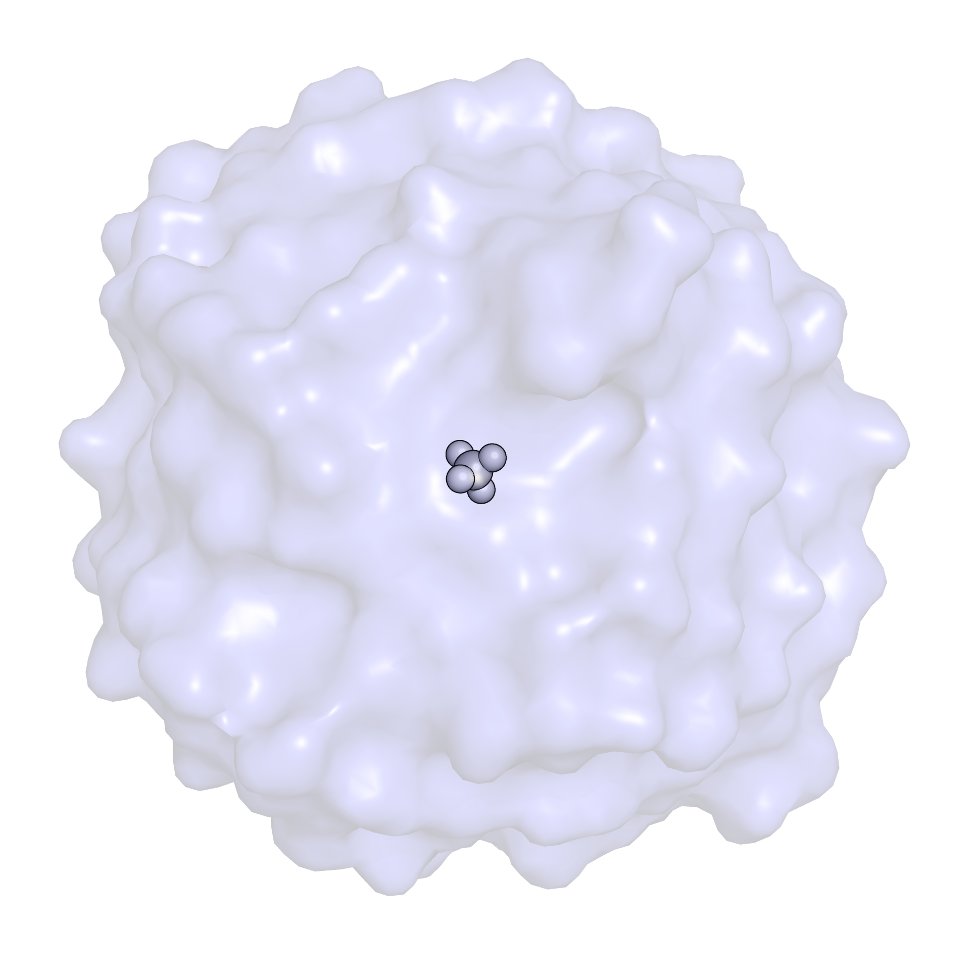
\includegraphics{free_energy_methane_water}
\caption{A single methane molecule (CH\textsubscript{4}) in water.}
\label{free_energy_methane_water_fig}
\end{figure}

In Section~\ref{pmf}, the concept of computing a free energy difference along a reaction coordinate was introduced. There is another type of free energy calculation frequently employed in MD simulations, in which a set of atoms is transformed in some manner from one state to another (typically denoted A and B), yielding some difference in free energy that relates to this change in topology. Common applications include mutating one small molecule to another and computing a $\Delta\Delta$G of binding (a relative free energy difference) or by turning off all interactions between some molecule and the remaining system, yielding $\Delta$G of solvation in that system (an absolute free energy difference). The free energy difference between two states, A and B, was originally defined by Zwanzig~\cite{Zwanzig1954}:

\begin{equation} \label{fep_eq}
\Delta G(A \longrightarrow B) = G_B - G_A = -k_B T \left \langle exp \left(-\frac{E_B - E_A}{k_B T}\right)\right \rangle_A
\end{equation}

That is, for every configuration generated in state A, the energy of the system is also evaluated in state B, from which the free energy difference, $\Delta$G, is calculated. This approach is called free energy perturbation (FEP). The drawback to the approach is that convergence is difficult unless the difference between the two states is small. For "mutation" of one molecule into another, or to transform a molecule from a fully interacting to a non-interacting state, this approach may fail to converge. In practice, such a calculation of a free energy difference is actually a series of MD simulations, in which the molecule of interest progressively has its topology changed from state A to state B as a function of a discrete coupling factor, $\lambda$. In these simulations, the Hamiltonian $H(\mathbf{r}, \mathbf{p})$ in terms of atomic coordinates ($\mathbf{r}$) and momenta ($\mathbf{p}$) is extended to include $\lambda$, {\em e.g.} $H(\mathbf{r}, \mathbf{p}; \lambda)$. For a given value of $\lambda$ (which takes values from 0 to 1, indicating fully in the A-state and fully in the B-state, respectively), the Hamiltonian of the system is expressed as:

\begin{equation} \label{fes_hamiltonian_eq}
H(\mathbf{r},\mathbf{p};\lambda) = (1 - \lambda) H^A(\mathbf{r},\mathbf{p}) + \lambda H^B(\mathbf{r},\mathbf{p})
\end{equation}

This approach to determining free energy differences is often called an "alchemical transformation," as it involves unphysical intermediates. For example, when determining $\Delta$G of solvation, state A ($\lambda = 0$) would correspond to the solute in a non-interacting state. In other words, the molecule experiences intramolecular interactions but no intermolecular interactions ({\em e.g.} solute-solvent) such that it samples the ideal gas state. State B ($\lambda = 1$) would then correspond to the fully interacting state, in which all nonbonded interactions are at full strength. Setting $\lambda = 0.5$ indicates that intermolecular interactions are at half strength, but how does one define a molecule that is halfway interacting with its surrounding environment? These are unphysical intermediates. However, since $\Delta$G is a state function, it does not matter what path is taken to arrive at the final answer, and the purpose of these intermediates is to define changes in energy that are small enough that they allow for convergence of the calculation.

Another method used to evaluate free energy differences is thermodynamic integration (TI), wherein the same $\lambda$-dependent transformation is carried out, and the quantity $\frac{\partial H(\lambda)}{\partial \lambda}$ is stored. After the simulations are finished, the integral is taken over the entire $\lambda$ range:

\begin{equation} \label{ti_eq}
\Delta G = \int_{0}^{1} \left\langle \frac{\partial H(\lambda)}{\partial \lambda} \right\rangle d\lambda
\end{equation}

The method used for computing $\Delta$G in this tutorial is the Bennett Acceptance Ratio (BAR)~\cite{Bennett1976}. Bennett originally formulated this method for Monte Carlo (MC) simulations, however it is easily extended to MD simulations, which are essentially MC simulations in which all trial moves are accepted. The BAR method is based on an assumption that states A and B share the same microstates, though the energies of these microstates are different. Bennett subsequently demonstrated that for functions satisfying detailed balance, one can compute the free energy change between states from the Metropolis function in the simplest case:

\begin{equation} \label{metropolis_eq}
M(x) \equiv min(e^{-x}, 1)
\end{equation}
%
such that

\begin{equation} \label{bar_simplest_eq}
e^{-\beta\Delta G} = \frac{\left\langle M\left(\beta\left(U_B - U_A\right)\right)\right\rangle_A}{\left\langle M\left(\beta\left(U_A - U_B\right)\right)\right\rangle_B}
\end{equation}
%
where $\beta = (k_B T)^{-1}$ and the angle brackets denote the ensemble averages over the configurations in states A and B.

Bennett demonstrates that in the more general case, in which some function, $f$, is used that includes some unknown free energy offset, $C$:

\begin{equation} \label{bar_general_eq}
e^{-\beta(\Delta G - C)} = \frac{\left\langle f\left(\beta\left(U_B - U_A - C\right)\right)\right\rangle_A}{\left\langle f\left(\beta\left(U_A - U_B + C\right)\right)\right\rangle_B}
\end{equation}
%
that the free energy can be estimated with minimum error when the chosen function is the Fermi function:

\begin{equation} \label{bar_fermi_eq}
f(x) = \frac{1}{1 + e^x}
\end{equation}
%
which, when used in Equation~\ref{bar_general_eq}, and solving iteratively after an initial estimate for $C$, yields:

\begin{equation} \label{bar_final_eq}
\Delta G \approx C
\end{equation}

This tutorial (available online at \tutorialfes) will guide the user through the calculation of the free energy change associated with removing van der Waals interactions of methane with water (Figure~\ref{free_energy_methane_water_fig}) using the BAR algorithm, implemented in GROMACS as the \texttt{bar} program. This quantity is part of the total transformation of methane that would be used to compute the complete free energy of solvation, $\Delta$G\textsubscript{solv}. This quantity has been rigorously calculated by Shirts et al. using the TI method~\cite{Shirts2003}.

\subsubsection{System Contents} \label{fes_top}

The system considered here contains a single methane (CH\textsubscript4) molecule solvated in 596 water molecules (Figure~\ref{free_energy_methane_water_fig}). The OPLS-AA force field~\cite{Kaminski2001} is used to describe methane and TIP3P~\cite{Jorgensen1983} is the water model. The coordinate and topology files for the system are available from the online version of this tutorial. A brief description of the topology contents is warranted here. The following describes the methane \texttt{[moleculetype]}:

\begin{lstlisting}[basicstyle=\footnotesize\ttfamily]
[ moleculetype ]
; Name                       nrexcl
Methane                      3

[ atoms ]
; nr      type resnr residue atom cgnr  charge    mass
   1  opls_138     1   ALAB    CB    1   0.000  12.011   
   2  opls_140     1   ALAB   HB1    2   0.000   1.008   
   3  opls_140     1   ALAB   HB2    3   0.000   1.008   
   4  opls_140     1   ALAB   HB3    4   0.000   1.008   
   5  opls_140     1   ALAB   HB4    5   0.000   1.008
\end{lstlisting}

The residue is named "ALAB," from the $\beta$-carbon of alanine, for which methane serves as a model compound. All of the charges on the atoms are set to zero, though strictly speaking, it is not necessary to do so. This tutorial will only consider the van der Waals transformation (that is, turning off Lennard-Jones interactions as a function of $\lambda$). In past versions of GROMACS (e.g. 4.0 and earlier), to do such a transformation would have required a topology with the form shown here, so that Coulombic interactions are not included. As will be explained below, charges can be present in the topology but also ignored. Should the user wish to perform a full transformation to calculate $\Delta$G\textsubscript{solv}, appropriate charges for all H atoms are +0.060 and -0.240 for the C atom. The topology shown here corresponds to the A-state of the molecule, such that it is fully interacting with its environment. It is also not necessary to specify a B-state in the topology (as was the case in past GROMACS versions, as well) since the transformation of nonbonded terms is controlled entirely in the \texttt{.mdp} file. A relative free energy calculation, in which one molecule is "mutated" to another, does require explicit B-state parameters (atom types and charges) to be set. Such a calculation is beyond the scope of this tutorial.

\subsubsection{Free Energy Settings} \label{fes_settings}

Every \texttt{.mdp} file used in this tutorial has a section with the following form:

\begin{lstlisting}[basicstyle=\footnotesize\ttfamily]
free_energy              = yes
init_lambda_state        = 0
delta_lambda             = 0
calc_lambda_neighbors    = 1
couple-moltype           = Methane
couple-lambda0           = vdw
couple-lambda1           = none
couple-intramol          = no
vdw_lambdas              = 0.00 0.05 0.10 0.15 ...
coul_lambdas             = 0.00 0.00 0.00 0.00 ...
bonded_lambdas           = 0.00 0.00 0.00 0.00 ...
restraint_lambdas        = 0.00 0.00 0.00 0.00 ...
mass_lambdas             = 0.00 0.00 0.00 0.00 ...
temperature_lambdas      = 0.00 0.00 0.00 0.00 ...
sc-alpha                 = 0.5
sc-coul                  = no
sc-power                 = 1
sc-sigma                 = 0.3
nstdhdl                  = 10
\end{lstlisting}

The \texttt{free\_energy} keyword instructs \texttt{grompp} to read the relevant free energy settings. If this keyword is set to \texttt{no}, then all the options shown are ignored. The \texttt{init\_lambda\_state} determines the value of $\lambda$, which is actually a vector, as explained below. The \texttt{delta\_lambda} keyword allows $\lambda$ to change as a function of time, in what are called "slow-growth" free energy calculations. Such a feature will not be used in this tutorial. The \texttt{calc\_lambda\_neighbors} keyword will instruct \texttt{mdrun} on how many neighboring values of $\lambda$ it should evaluate the energy of the system. Recall from Equation~\ref{bar_general_eq} that the energies of A- and B-states for a given configuration are needed. It is also possible to use multiple neighboring states (discussed below). For standard BAR, only a single neighbor needs its energy evaluated under the B-state topology.

The \texttt{couple-moltype} specifies the \texttt{[moleculetype]} name that will have its topology transformed as a function of $\lambda$. The \texttt{couple-lambda0} and \texttt{couple-lambda1} keywords specify which interactions are on in the A- and B-states, respectively. Valid options for these keywords are \texttt{vdw-q} (meaning both vdW and Coulombic interactions are fully on), \texttt{vdw} (only vdW), \texttt{q} (only Coulombic), and \texttt{none} (no intermolecular interactions; the coupled \texttt{[moleculetype]} is non-interacting, {\em i.e.} in the ideal gas state). The \texttt{couple-intramol} setting determines whether or not intramolecular nonbonded interactions are to be transformed as a function of $\lambda$. For small molecules, this option is typically set to \texttt{no} such that the fully transformed state still corresponds to the ideal gas state. Larger molecules may become trapped in a narrowly defined conformational ensemble, requiring softening of intramolecular nonbonded interactions, in which case \texttt{couple-moltype} might be set to \texttt{yes}. Methane has no intramolecular nonbonded interactions, so this setting will not affect the outcome, but for larger molecules it may be relevant.

From these options, the transformation of methane is now defined. The A-state corresponds to a molecule that interacts with water only via vdW interactions (\texttt{couple-moletype0 = vdw}). This setting is why it is irrelevant if charges are defined in the topology; even if present, they will be ignored. In the B-state, methane is non-interacting (\texttt{couple-moltype1 = none}), so the $\Delta$G calculated in this series of simulations will correspond to the vdW contribution to $-\Delta$G\textsubscript{solv}. $\Delta$G\textsubscript{solv} is formally defined as the free energy change associated with the introduction of a solute into solvent, which would be specified by inverting the definitions of the A- and B-states defined here.

The next set of options define the $\lambda$ vector for nonbonded interactions (vdW and Coulombic) as well as bonded terms and restraints, masses of atoms, and the temperature of the system. Scaling temperatures is only relevant for simulated tempering~\cite{Marinari1992,Geyer1995}, which will not be discussed in this tutorial. These settings are used to define the $\lambda$ vector, which is indexed with the \texttt{init\_lambda\_state} keyword. Vectors are zero-based indices, so $\lambda$[0] = (0.00, 0.00, 0.00, 0.00, 0.00, 0.00), $\lambda$[1] = (0.05, 0.00, 0.00, 0.00, 0.00, 0.00) and so on, corresponding to each column of values in the \texttt{*\_lambdas} arrays. Though charges are not being transformed in this example, it is important to note that in such a case, charges should not be present on atoms that have no vdW terms to avoid numerical instability. That is, charges should only ever be "on" for atoms that have full vdW interactions. For this reason, setting \texttt{couple-moltype* = q} is very uncommon.

The options starting with \texttt{sc-} define parameters associated with "soft-core" modification of potentials~\cite{Beutler1994}. As $\lambda$ increasingly defines atoms with no vdW radii or very weak charges (in the absence of vdW terms), it is possible for atoms to overlap, leading to a numerical singularity (infinite force). While all $\lambda$-dependent transformations inherently sample unphysical states, a singularity makes calculation of the forces impossible and therefore must be prevented. To circumvent this problem, nonbonded potentials can be shifted, as shown in Equation~\ref{sc_eq} for the Lennard-Jones form of vdW interactions: 
\begin{equation} \label{sc_eq}
\footnotesize
U_{ij}^{LJ} (r_{ij};\lambda) = 4\epsilon\lambda^p\left(\left[\alpha(1-\lambda)^p + \left(\frac{r_{ij}}{\sigma_{ij}}\right)^6\right]^{-2} - \left[\alpha(1-\lambda)^p + \left(\frac{r_{ij}}{\sigma_{ij}}\right)^6\right]^{-1}\right)
\end{equation}

The \texttt{sc-alpha} keyword sets the value of $\alpha$ in Equation~\ref{sc_eq}. The \texttt{sc-power} option sets the value of $p$; here, this parameter is set to 1 to indicate a linear dependence on $\lambda$, which has been shown to be a robust approach in conjunction with $\alpha = 0.5$~\cite{Pitera2002,Steinbrecher2007,Shirts2005}. The \texttt{sc-sigma} keyword specifies a value of $\sigma$ for atoms that have force field parameter values of $\sigma$ less than this specified value. This setting is important for atoms like hydrogen, which often do not have their own Lennard-Jones parameters. The final option, \texttt{sc-coul}, is not relevant here as charges are not being transformed. Typically, soft-core modifications are not applied to Coulombic interactions, if the transformation is being carried out on atoms that still have vdW interactions (the recommended approach). However, if one is transforming charges on atoms that do not have vdW interactions, the soft-core modification is recommended to avoid the same numerical singularity problems described above.

The last setting in this section of the \texttt{.mdp} file, \texttt{nstdhdl}, simply specifies the interval (in number of time steps) for writing the values of $\frac{\partial H(\lambda)}{\partial \lambda}$ to the output file.

\subsubsection{Workflow} \label{fes_workflow}

The calculation of $\Delta$G for removing vdW interactions between methane and water will be carried out in 21 individual simulations, one for each of the $\lambda$ vectors defined in the \texttt{.mdp} files. Preceding each production simulation, the system will be energy-minimized, then equilibrated under an $NVT$ and then an $NPT$ ensemble for 100 ps each. Following these preparation steps, the production MD simulations (during which data are collected) will be carried out for 1 ns.

In this example, the values of $\lambda$ are spaced equally from 0 to 1, thus an interval of 0.05. It is typical to cluster values of $\lambda$ towards each of the end states, using a finer spacing to better resolve the energies of the fully and non-interacting states. For simplicity and in the interest of time, equal spacing is used here. As will be shown below, in this very simple case, such a $\lambda$ spacing is adequate, but this may not always be the case.

The online tutorial provides a Bash script (\texttt{job.sh}) to run each of these jobs in a loop, though it is not necessary to do so. As all of the simulations are independent, it is possible to run them all simultaneously if preferred. All of the \texttt{.mdp} settings should be familiar by now, though it is important to note the use of the \texttt{sd} integrator (for "stochastic dynamics," more commonly called "Langevin dynamics"). A random frictional force is applied to all the atoms with an inverse friction coefficient specified by \texttt{tau\_t}, which has been set to 1.0 ps\textsuperscript{$-$1}, to avoid over-damping of water and subsequently artificially impacting sampling. Do not use a value smaller than 1.0 here.

\subsubsection{Analysis} \label{fes_ana}

Collect all of the output \texttt{md*.xvg} files from the production MD runs into one directory and execute the \texttt{bar} program:

\begin{lstlisting}
$ gmx bar -f md*.xvg -o -oi
\end{lstlisting}

The \texttt{bar} program prints free energy differences for each $\lambda$ window to the terminal (including entropy in each window, all in units of kT). At the end of the printed information will be the final results, in kJ mol\textsuperscript{$-$1}:

\begin{lstlisting}
Final results in kJ/mol:

point      0 -      1,   DG  0.19 +/-  0.00
point      1 -      2,   DG  0.17 +/-  0.01
point      2 -      3,   DG  0.14 +/-  0.00
point      3 -      4,   DG  0.09 +/-  0.01
point      4 -      5,   DG  0.06 +/-  0.00
point      5 -      6,   DG  0.01 +/-  0.01
point      6 -      7,   DG -0.06 +/-  0.01
point      7 -      8,   DG -0.14 +/-  0.02
point      8 -      9,   DG -0.23 +/-  0.01
point      9 -     10,   DG -0.35 +/-  0.01
point     10 -     11,   DG -0.53 +/-  0.01
point     11 -     12,   DG -0.77 +/-  0.03
point     12 -     13,   DG -1.12 +/-  0.03
point     13 -     14,   DG -1.46 +/-  0.02
point     14 -     15,   DG -1.53 +/-  0.04
point     15 -     16,   DG -1.35 +/-  0.02
point     16 -     17,   DG -1.04 +/-  0.01
point     17 -     18,   DG -0.70 +/-  0.01
point     18 -     19,   DG -0.40 +/-  0.00
point     19 -     20,   DG -0.13 +/-  0.00

total      0 -     20,   DG -9.13 +/-  0.09
\end{lstlisting}

The transformation carried out here was the disappearance of vdW terms in methane, the opposite of the vdW contribution to the solvation free energy. Converting the obtained result to kcal mol\textsuperscript{$-$1} and inverting the sign (assuming reversibility of this process), the final result is 2.18 $\pm$ 0.02 kcal mol\textsuperscript{$-$1}, in good agreement with the value obtained by Shirts et al. of 2.21 $\pm$ 0.01 kcal mol\textsuperscript{$-$1}~\cite{Shirts2003}. Small differences can be attributed to different software versions, cutoff schemes, integration algorithms, different $\lambda$ spacing, and thermostats. However, the close agreement between these two results indicates that the present approach is robust and can reproduce the known quantity sufficiently.

The \texttt{-o} and \texttt{-oi} arguments produce \texttt{bar.xvg} and \texttt{barint.xvg}, the free energy differences as a function of $\lambda$ state and the integral of these free energy differences (which gives the total $\Delta$G for the transformation). It is also possible to output histograms of the free energy differences, but this output will not be discussed in this tutorial. The plot of $\Delta$G as a function of $\lambda$ is shown in Figure~\ref{free_energy_plot_bar_fig}.

\begin{figure}[h!]
\centering
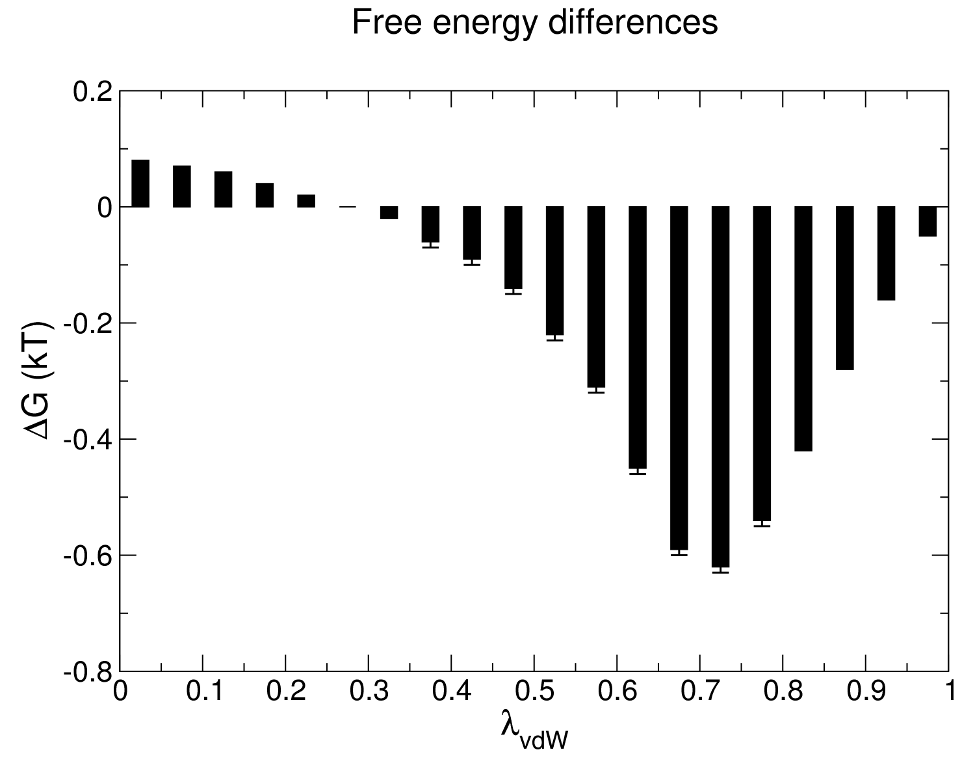
\includegraphics{free_energy_plot_bar}
\caption{The $\Delta$G values for each $\lambda$ window, from the BAR algorithm.}
\label{free_energy_plot_bar_fig}
\end{figure}

Note that the default $x$-axis will be integers, corresponding to the indices of the $\lambda$ vector. These values have been replaced in Figure~\ref{free_energy_plot_bar_fig} with the specific values of \texttt{vdw-lambdas} in each of these $\lambda$ vectors. Recall that no other energy terms were transformed as a function of $\lambda$, so the free energy changes are all one-dimensional, and referred to simply as $\lambda$\textsubscript{vdW} for clarity. Each value is plotted between two discrete values of $\lambda$. The BAR algorithm evaluates free energy differences between the neighboring $\lambda$ values, so the $\Delta$G values correspond to the free energy difference of a given configuration evaluated under the A- and B-state topologies (calculated every \texttt{nstdhdl} steps, see Section~\ref{fes_settings}). The plotted BAR output corresponds to $\Delta$G values between $\lambda = 0$ and $\lambda = 0.05$, $\lambda = 0.05$ and $\lambda = 0.1$, and so on.

The integral of these values is plotted in Figure~\ref{free_energy_plot_barint_fig}, to accumulate $\Delta$G as a function of $\lambda$. The final value is -3.69 k\textsubscript{B}T, or -9.14 kJ mol\textsuperscript{$-$1}, since k\textsubscript{B}T = 2.478 kJ mol\textsuperscript{$-$1} at 298 K. This value agrees with the value previously printed to the terminal by the \texttt{bar} program (-9.13 kJ mol\textsuperscript{$-$1}). The values are not exactly the same because the calculation done by the \texttt{bar} program is carried out with greater precision than using just two, rounded decimal places printed to the screen.

\begin{figure}[h!]
\centering
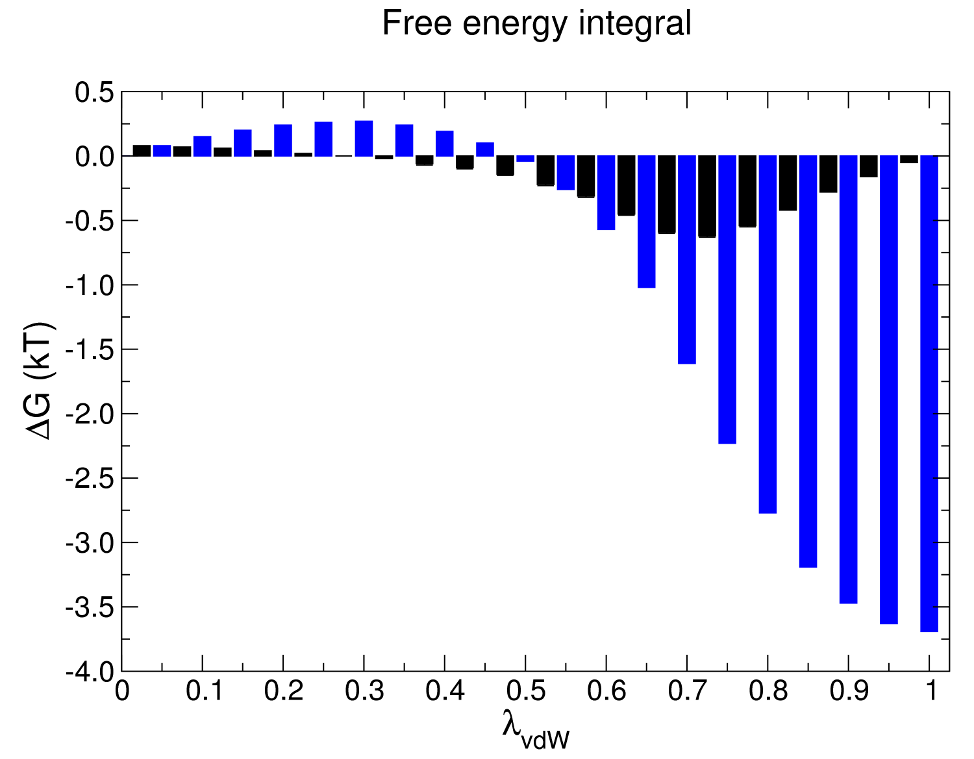
\includegraphics{free_energy_plot_barint}
\caption{The cumulative $\Delta$G value (blue), plotted along with $\Delta$G values from each $\lambda$ window (black), from the BAR algorithm.}
\label{free_energy_plot_barint_fig}
\end{figure}

\subsubsection{More Advanced Free Energy Calculations} \label{fes_advanced}

Common applications of free energy calculations via MD simulation include full solvation free energies and binding free energies. To obtain $\Delta$G\textsubscript{solv} for methane, the user would simply include charges in the system topology and set up a series of \texttt{coul-lambdas} in the \texttt{.mdp} files. The \texttt{bar} program can be then called in the same manner to obtain the total value of $\Delta$G\textsubscript{solv}.

Computing a binding free energy between a ligand and a protein is beyond the scope of this tutorial, but interested readers are directed to \url{http://www.alchemistry.org/wiki/Main_Page}, which has all the information necessary to perform these calculations. The most challenging aspect of these kinds of calculations is the need to restrain the ligand as it is slowly transformed. Non- or weakly interacting states of the ligand will begin to diffuse through the protein and sample totally unphysical regions of the system, inhibiting convergence of the calculations. To circumvent this problem, distance and orientational restraints can be imposed on the ligand as a function of $\lambda$. The energetic contributions of the restraints to the free energy can be corrected analytically after the simulations. An example of such a process is described by Jo et al. in their implementation of the CHARMM-GUI Ligand Binder~\cite{Jo2012}. See also references therein. The difference between the computed free energy difference from transforming the ligand in the binding site of the protein ($\Delta$G\textsubscript{complexation}) and the solvation free energy of the ligand ($\Delta$G\textsubscript{solv}) yields the binding free energy, $\Delta$G\textsubscript{bind}.

\subsubsection{Summary and Review of Objectives} \label{fes_summary}

This tutorial has guided the user through the process of calculating the free energy change associated with turning off vdW interactions between methane and water. The free energy change was computed with the BAR algorithm~\cite{Bennett1976}. To review, the learning objectives of the tutorial are:

\begin{enumerate}
	\item Understand the purpose of \texttt{.mdp} keywords related to free energy calculations
	\item Use the Bennett Acceptance Ratio method to compute the free energy difference of the transformation of van der Waals terms
\end{enumerate}

The user was introduced to settings related to free energy in Section~\ref{fes_settings} and analysis using BAR was performed in section~\ref{fes_ana}. Several output files were plotted and their contents discussed. Interested readers may wish to refer to the Multistate BAR (MBAR) method~\cite{Shirts2008}, in which free energy differences are computed from all states. A Python implementation for MBAR is available from \url{https://github.com/choderalab/pymbar} and is fully compatible with GROMACS output. The user simply needs to increase the value of \texttt{calc\_lambda\_neighbors} in the \texttt{.mdp} file to evaluate free energy differences among all $\lambda$ states.



%%%%%%%%% TUTORIAL 7 %%%%%%%%%
\subsection{Tutorial 7: Virtual Sites} \label{vsite}

\begin{figure}[h]
\centering
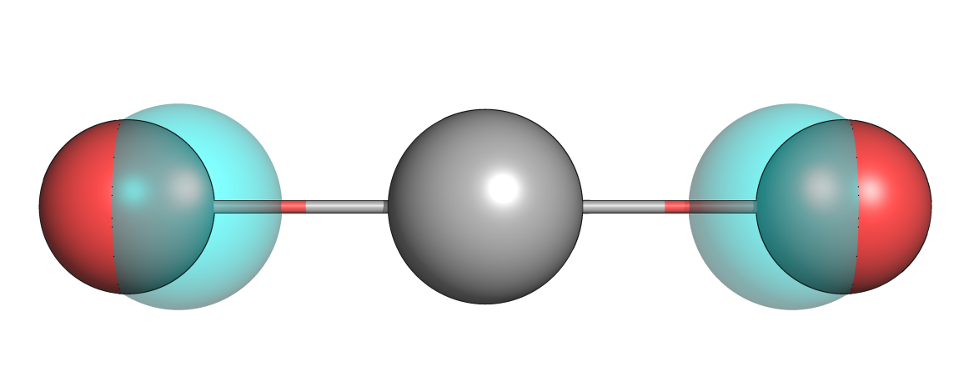
\includegraphics{vsites_co2}
\caption{The CO\textsubscript{2} molecule, with two mass centers (cyan) that are used to construct virtual sites that replace the C and O atoms.}
\label{vsites_co2_fig}
\end{figure}

In this tutorial (available online at \tutorialvsite), the user will be guided through the process of constructing a linear, triatomic molecule (CO\textsubscript{2}) using two massive particles and converting the C and O atoms into virtual sites (Figure~\ref{vsites_co2_fig}). A virtual site is a type of particle that has the following characteristics:

\begin{enumerate}
	\item It has no mass
	\item It may participate in Lennard-Jones and/or charge interactions
	\item Any forces acting on virtual sites are projected onto their constructing atoms
	\item Virtual site positions are not integrated, they are computed from updated positions of constructing atoms
\end{enumerate}

In some literature, virtual sites are referred to as "dummy atoms," though this term is somewhat imprecise and can refer to generic, non-interacting particles. Be aware of this convention, as some articles are ambiguous in their usage.

Virtual sites have various applications in simulation literature. The first is to construct linear molecules, which present an algorithmic difficulty - the force discontinuity in evaluating the cosine of the angle $i-j-k$ as it changes sign by fluctuating around 180\textdegree. It is this application that is explored in the present tutorial. Virtual sites are also used to define the positions of lone pairs on electronegative atoms, which exist as regions of electron density at predictable locations around these atoms. Examples include the modeling of the $\sigma$-hole on halogens in the OPLS3~\cite{Harder2016} and CGenFF~\cite{Gutierrez2016} parameter sets, lone pairs on sulfur atoms in OPLS-AA and OPLS/CM5~\cite{Yan2017}, in modeling hydrogen-bond acceptors in the Drude polarizable force field~\cite{Harder2006,Lemkul2016}, and in repartitioning hydrogen masses onto heavier atoms to increase the time step used in MD simulations~\cite{Feenstra1999,Bjelkmar2010}.

The procedure undertaken in this tutorial is quite different from all of the previous examples. There will be no use of \texttt{pdb2gmx} to write a topology, as it will be written manually by the user. There will be only one MD simulation that is performed in the absence of PBC to model the gas phase.

\subsubsection{Create the Topology} \label{vsite_top}

To create the model for CO\textsubscript{2}, the C and O atoms will be converted to virtual sites. They will participate in Lennard-Jones interactions and will have charges assigned to them, thereby interacting via normal Coulombic interactions with other particles. The forces acting on these virtual sites will be projected onto two mass centers, which have no charge or Lennard-Jones terms, serving only to receive the forces from the virtual sites and have their positions integrated during MD. The topology for CO\textsubscript{2} will be derived from the OPLS-AA force field. Charges are taken from work by Yang and Zhong~\cite{Yang2006}, combined with standard OPLS-AA atom types. The model developed by doing so has not been rigorously tested in any way, but serves as a viable model for the illustrative purposes of this tutorial.

A complete, functional topology is available from the online version of the tutorial. Here, each section of the topology will be derived and explained.

The structure of CO\textsubscript{2} is shown in Figure~\ref{vsites_triatomic_fig}, along with the nomenclature that will be used in this tutorial.

\begin{figure}[H]
\centering
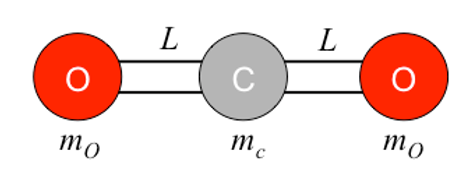
\includegraphics{vsites_triatomic}
\caption{A schematic of the CO\textsubscript{2} molecule, with bond length, $L$, between each C and O atom. The masses of the C and O atoms are $m_C$ and $m_O$, respectively.}
\label{vsites_triatomic_fig}
\end{figure}

Two properties have to be preserved in developing a virtual site model for CO\textsubscript{2}: the total mass and the moment of inertia. Assigning masses to the two mass centers is straightforward. The mass of CO\textsubscript{2} is 44.0098 amu (1 carbon atom at 12.011 amu and 2 oxygen atoms at 15.9994 amu, according to the masses assigned in the OPLS-AA force field). Therefore, each mass center will be assigned half of this mass, or 22.0049 amu.

A new atom type, MCO, is introduced in the topology to describe the mass centers. It has no Lennard-Jones parameters associated with it. The new atom type definition and the atoms of the topology are defined as follows (note that the mass listed in \texttt{[atomtypes]} is irrelevant and is set in \texttt{[atoms]}.:

\begin{lstlisting}[basicstyle=\footnotesize\ttfamily]
[ atomtypes ]
; name  bond_type mass  charge ptype    sigma   epsilon
  MCO   MCO       0.000 0.000  A        0.000   0.000

[ moleculetype ]
; name  nrexcl
CO2     2

[ atoms ]
; nr    type  resnr residue  atom cgnr   charge     mass
  1 opls_272      1    CO2     O1    1   -0.350   0.0000 
  2 opls_271      1    CO2      C    1    0.700   0.0000
  3 opls_272      1    CO2     O2    1   -0.350   0.0000
  4      MCO      1    CO2     M1    1    0.000  22.0049     
  5      MCO      1    CO2     M2    1    0.000  22.0049
\end{lstlisting}

A CO\textsubscript{2} molecule is essentially a linear, triatomic rotor, from which the moment of inertia, $I$, can be calculated as:

\begin{equation} \label{eq_rotor}
I = 2 m_O L^2
\end{equation}

The value of L is the C=O bond length, 0.125 nm. Substituting in the value of $m_O$ (15.9994 amu) yields a moment of inertia of 0.500 amu nm\textsuperscript{2}.

Next, the distance between the mass centers (Figure~\ref{vsites_masses_fig}) must be determined, such that the moment of inertia for the molecule is preserved.

\begin{figure}[H]
\centering
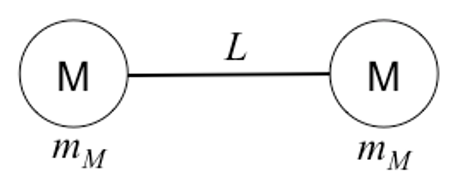
\includegraphics{vsites_masses}
\caption{A schematic of the mass-carrying sites that will be used to convert CO\textsubscript{2} into a diatomic, rigid rotor.}
\label{vsites_masses_fig}
\end{figure}

The equation for $I$ of a rigid rotor is:

\begin{equation} \label{eq_diatomic}
I = \left(\frac{m_M m_M}{m_{Total}}\right) L^2
\end{equation}

Solving for $L$ yields a value of 0.213173 nm, which is the length of the distance that will be assigned between the two mass centers. Rather than assigning this interaction as a normal harmonic bond (which would require the parametrization of a force constant, the physical relevance of which is not easily determined), the topology will assign a constraint such that the distance between the two mass centers is fixed. Doing so also makes it straightforward to construct the C and O virtual sites.

Thus, the constraint is defined in the topology as:

\begin{lstlisting}
[ constraints ]
    4   5   1   0.213173
\end{lstlisting}

The C virtual site is assigned exactly in the middle of the two mass centers. In GROMACS, virtual sites can be constructed in a linear form by specifying the location of the virtual site as a fraction of the distance, $a$, between two constructing atoms. Therefore, the C virtual site will be exactly halfway between the two mass centers, or half of the assigned constraint length. Within a \texttt{[virtual\_sites2]} directive: 

\begin{lstlisting}
[ virtual_sites2 ]
; site  ai  aj  funct   a
     2   4   5      1   0.5000
\end{lstlisting}

Last, the positions of the O virtual sites must be defined, again expressed as a fraction of the bond distance between the mass centers, M1 and M2. Since the C virtual site is 0.1065865 nm away from each M, and the C=O bond length is 0.125 nm, each O virtual site must be constructed 0.0184135 beyond the M1-M2 distance. This distance must be expressed as a fraction of the M1-M2 constraint length, therefore:

\begin{equation}
a = \frac{0.213173+0.0184135}{0.213173} = 1.0851116
\end{equation}

Now, the O virtual site constructions can be added to the \texttt{[virtual\_sites2]} directive:

\begin{lstlisting}
[ virtual_sites2 ]
; site  ai  aj  funct   a
     1   4   5      1   1.0851116
     2   4   5      1   0.5000 
     3   5   4      1   1.0851116
\end{lstlisting}

Note that the order of the constructing atoms (M1 and M2) in this directive specifies the direction of the vector along which the O virtual sites are constructed. O site 1 is constructed beyond M2 (outside of the M1-M2 constraint) and O site 3 is constructed beyond M1 (outside the M2-M1 constraint).

\subsubsection{Simple MD Simulation} \label{vsite_md}

To validate the approach, a small gas-phase system of CO\textsubscript{2} will be constructed. Place 10 molecules in a large box:

\begin{lstlisting}
$ gmx insert-molecules -ci co2.pdb -nmol 10 -box 10 10 10 -o box.pdb
\end{lstlisting}

Energy minimization and the subsequent MD simulation will be carried out without periodicity and "infinite" cutoffs, to mimic a gas-phase system. The relevant \texttt{.mdp} options in both \texttt{em.mdp} and \texttt{md.mdp} are:

\begin{lstlisting}
cutoff-scheme   = group
nstlist         = 0
ns_type         = simple
rlist           = 0
coulombtype     = cutoff
rcoulomb        = 0
rvdw            = 0
pbc             = no
\end{lstlisting}

During MD, angular momentum is also conserved:

\begin{lstlisting}
comm-mode       = angular
\end{lstlisting}

Setting \texttt{nstlist} to zero means the neighbor list is fixed. All interatomic interactions are considered in this simulation. This approach differs from the truncation schemes utilized in condensed-phase systems that have far more atoms, making this approach intractable if there are many atoms. For gas-phase systems, where there are few atoms and therefore few interactions, it is possible (and physically meaningful) to use the settings listed above.

Perform energy minimization:

\begin{lstlisting}
$ gmx grompp -f em.mdp -c box.pdb -p topol.top -o em.tpr

$ gmx mdrun -nt 1 -nb cpu -deffnm em
\end{lstlisting}

Note that the use of the group cutoff scheme prevents the use of a GPU, hence the use of \texttt{-nb cpu} to tell \texttt{mdrun} to only use CPU hardware. Only one thread is started since the system only contains 50 particles. It will not benefit from parallelization.

Continue with MD:

\begin{lstlisting}
$ gmx grompp -f md.mdp -c em.gro -p topol.top -o md.tpr

$ gmx mdrun -nt 1 -nb cpu -deffnm md
\end{lstlisting}

When the simulation is finished, analyze the moments of inertia of CO\textsubscript{2} to verify that the approach worked. First, create an index file by splitting all of the CO\textsubscript{2} molecules into their own groups so they can be analyzed individually:

\begin{lstlisting}
$ gmx make_ndx -f em.gro
> splitres 0
> q
\end{lstlisting}

Use the GROMACS \texttt{principal} program to compute the moments of inertia. Choose any of the CO\textsubscript{2} molecules from the index file when prompted.

\begin{lstlisting}
$ gmx principal -s md.tpr -f md.trr -n index.ndx
\end{lstlisting}

The output file, \texttt{moi.xvg}, contains moments of inertia around the $x$-, $y$-, and $z$-axes. Rotation around $x$ is zero, because this axis coincides with the M1-M2 constraint. The $y$- and $z$- moments are 0.500, in exact agreement with the value computed above. This outcome indicates that the approach taken to convert a triatomic molecule into a rigid, diatomic rotor is physically reasonable.

\subsubsection{Summary and Review of Objectives} \label{vsite_summary}

In this tutorial, the concept of virtual sites was introduced by converting a triatomic molecule, CO\textsubscript{2}, into a linear, rigid rotor. Two mass centers were constructed using a rigid constraint, from which three virtual sites, representing C and O atoms, were constructed. To review, the learning objectives of the tutorial are:

\begin{enumerate}
	\item Define a virtual site and its position relative to other atoms
	\item Construct a system of a linear molecule with virtual sites
\end{enumerate}

The concept of virtual sites was introduced in Section~\ref{vsite} and demonstrated in Section~\ref{vsite_top} through the manual construction of a topology file and coordinates. The utility and accuracy of the approach was demonstrated with a simple, gas-phase MD simulation, in which the moments of inertia of CO\textsubscript{2} molecules were calculated.

% \section{Checklists}
% Tutorials do not necessarily require the use of a checklist as in Best Practices documents; however, they can include these if desired.
% Several useful checklist formats are available, with examples presented in \texttt{sample-document.tex} in \url{github.com/livecomsjournal/article_templates/templates}.
% One example is shown here.

% Here is a single-column checklist that consists of multiple sub-checklists
% \begin{Checklists}
% 
% \begin{checklist}{A list}
% \textbf{Single-column checklists are also straightforward by removing the asterisk}
% \begin{itemize}
% \item First thing let's do an item which breaks across lines to see how that looks
% \item Also remember
% \item And finally
% \end{itemize}
% \end{checklist}
% 
% \begin{checklist}{Another list}
% \textbf{This is some further description.}
% \begin{itemize}
% \item First thing
% \item Also remember
% \item And finally
% \end{itemize}
% \end{checklist}
% 
% \end{Checklists}

\section{Author Contributions}
%%%%%%%%%%%%%%%%
% This section must describe the actual contributions of
% author. Since this is an electronic-only journal, there is
% no length limit when you describe the authors' contributions,
% so we recommend describing what they actually did rather than
% simply categorizing them in a small number of
% predefined roles as might be done in other journals.
%
% See the policies ``Policies on Authorship'' section of https://livecoms.github.io
% for more information on deciding on authorship and author order.
%%%%%%%%%%%%%%%%

JAL conceived of and wrote all the online tutorials, composed the underlying HTML for \tutorialhomeurl, and wrote this article.

% We suggest you preserve this comment:
For a more detailed description of author contributions,
see the GitHub issue tracking and changelog at \githubrepository.

\section{Other Contributions}
%%%%%%%%%%%%%%%
% You should include all people who have filed issues that were
% accepted into the paper, or that upon discussion altered what was in the paper.
% Multiple significant contributions might mean that the contributor
% should be moved to authorship at the discretion of the a
%
% See the policies ``Policies on Authorship'' section of https://livecoms.github.io for
% more information on deciding on authorship and author order.
%%%%%%%%%%%%%%%

JAL thanks the many users of the GROMACS tutorials, who have provided important feedback and requests since the initial publication of the lysozyme tutorial in 2008, Dr. David R. Bevan for encouraging the development of these tutorials and hosting them on his lab web server for many years, and Dr. Anne M. Brown for providing technical assistance in maintaining tutorial accessibility while the tutorials were hosted on the Bevan lab website. JAL also thanks Dr. Michael Shirts for critical evaluation of Tutorial 6, "Free Energy of Solvation," prior to its online publication, and members of the Lemkul lab for critical review of this manuscript.

% We suggest you preserve this comment:
For a more detailed description of contributions from the community and others, see the GitHub issue tracking and changelog at \githubrepository.

\section{Potentially Conflicting Interests}
%%%%%%%
%Declare any potentially competing interests, financial or otherwise
%%%%%%%

JAL is a developer of the GROMACS simulation package.

\section{Funding Information}
%%%%%%%
% Authors should acknowledge funding sources here. Reference specific grants.
%%%%%%%
JAL thanks the NSF MILES-IGERT and Virginia Tech ICTAS Doctoral Scholars programs for financial support from 2007-2012, during which time the original tutorials were created. JAL is supported by startup funding from the Virginia Tech Office of the Provost, College of Agriculture and Life Sciences, and Department of Biochemistry and USDA National Institute of Food and Agriculture.

\bibliography{gmx-tutorials-refs}

%%%%%%%%%%%%%%%%%%%%%%%%%%%%%%%%%%%%%%%%%%%%%%%%%%%%%%%%%%%%
%%% APPENDICES
%%%%%%%%%%%%%%%%%%%%%%%%%%%%%%%%%%%%%%%%%%%%%%%%%%%%%%%%%%%%

%\appendix


\end{document}
